%! TEX program = xelatex
% 
% Versi 1.1
%
% Template Tugas Akhir 
% Program Studi Sistem dan Teknologi Informasi
% Sekolah Teknik Elektro dan Informatika
% Institut Teknologi Bandung
%
% --- oneside ditambahkan untuk menghilangkan blank page di seluruh dokumen ---
\documentclass[12pt,a4paper,oneside]{book}

% --- Main packages ---
\usepackage[utf8]{inputenc}
\usepackage{fontspec}
\usepackage[indonesian]{babel}
\usepackage{csquotes}
\usepackage{setspace}
\usepackage{graphicx}
\usepackage{caption}
\usepackage{subcaption}
\usepackage{tocloft}
\usepackage{titlesec}
\usepackage{lipsum}
\usepackage{floatrow}   % menyediakan [H]; JANGAN load package float (konflik)
\usepackage{listings}
\usepackage{amsmath}
\usepackage{amssymb}
\usepackage[shortlabels]{enumitem}
\usepackage[skip=12pt]{parskip}
\usepackage{longtable}
\usepackage{booktabs}
\usepackage[bahasai]{datetime2}
\usepackage{geometry}
\usepackage{algorithm}
\usepackage{algorithmicx}
\usepackage{algpseudocode}
\usepackage{microtype}
\usepackage{array}
\usepackage{threeparttable}
\usepackage{tabularx}
\usepackage{xcolor}
\usepackage[title,titletoc]{appendix}
\usepackage[hidelinks]{hyperref}

\setmainfont{Times New Roman}
\onehalfspacing

% --- Bibliography ---
\usepackage[
    backend=biber,
    authordate,
    language=english,
    autolang=other
]{biblatex-chicago}
\addbibresource{daftar-pustaka.bib}

% --- Terjemahan ke Bahasa Indonesia ---
\DefineBibliographyStrings{english}{
  and          = {dan},
  andothers    = {dkk.},
  editor       = {penyunting},
  editors      = {penyunting},
  translator   = {penerjemah},
  byeditor     = {disunting oleh},
  bytranslator = {diterjemahkan oleh},
  in           = {dalam},
  edition      = {edisi},
  pages        = {hal.},
  page         = {hal.},
  volume       = {vol.},
  number       = {no.},
  urlseen      = {diakses pada},
  url          = {tautan},
}

\let\oldcite\cite
\renewcommand{\cite}{\parencite}
\renewcommand*{\finalandcomma}{}

\hypersetup{
    colorlinks=true,
    linkcolor=black,
    citecolor=black,
    urlcolor=black
}

\pagestyle{plain}

% --- Listings ---
\renewcommand{\lstlistlistingname}{DAFTAR \textit{LISTING}}
\renewcommand{\lstlistingname}{\textit{Listing}}
\lstset{basicstyle=\ttfamily\footnotesize,breaklines=true}

% --- Algoritma ---
\renewcommand{\algorithmname}{Algoritma}
\renewcommand{\listalgorithmname}{DAFTAR ALGORITMA}
\renewcommand{\thealgorithm}{\thechapter.\arabic{algorithm}}

% --- Daftar Persamaan ---
\newlistof{myequations}{equ}{DAFTAR PERSAMAAN}
\setlength{\cftmyequationsnumwidth}{3em}
\renewcommand{\cftmyequationsaftersnum}{\hspace{0.5em}}
\newcommand{\eqcaption}[1]{%
  \addcontentsline{equ}{myequations}
  {\protect\numberline{\theequation}#1}
}
\makeatletter
\renewcommand{\listofmyequations}{%
  \chapter*{\centering\large\bfseries DAFTAR PERSAMAAN}
  \@starttoc{equ}
}
\makeatother

% --- TOC settings ---
\renewcommand \cftchapdotsep{4.5}
\setlength{\cftchapindent}{0em}
\setlength{\cftchapnumwidth}{1.8em}
\setlength{\cftsecindent}{1.8em}
\setlength{\cftsecnumwidth}{2.4em}
\setlength{\cftsubsecindent}{4.2em}
\setlength{\cftsubsecnumwidth}{2.8em}
\setlength{\cftsubsubsecindent}{7.0em}
\setlength{\cftsubsubsecnumwidth}{3.2em}

% --- Nama bulan Indonesia ---
\renewcommand*{\DTMbahasaimonthname}[1]{%
  \ifcase#1\or Januari\or Februari\or Maret\or April\or Mei\or Juni%
  \or Juli\or Agustus\or September\or Oktober\or November\or Desember\fi
}

% --- Margin ---
\geometry{a4paper, inner=4cm, outer=3cm, top=3cm, bottom=3cm}

% --- Listings style Python/C++ ---
\definecolor{codegreen}{rgb}{0,0.6,0}
\definecolor{codegray}{rgb}{0.5,0.5,0.5}
\definecolor{codepurple}{rgb}{0.58,0,0.82}
\definecolor{backcolour}{rgb}{0.95,0.95,0.92}

\lstdefinestyle{pythonstyle}{
    backgroundcolor=\color{backcolour},
    commentstyle=\color{codegreen},
    keywordstyle=\color{magenta},
    numberstyle=\tiny\color{codegray},
    stringstyle=\color{codepurple},
    basicstyle=\ttfamily\footnotesize,
    breakatwhitespace=false, breaklines=true,
    captionpos=b, keepspaces=true,
    numbers=left, numbersep=5pt,
    showspaces=false, showstringspaces=false,
    showtabs=false, tabsize=4,
    language=Python
}
\lstdefinestyle{cppstyle}{
    backgroundcolor=\color{backcolour},
    commentstyle=\color{codegreen},
    keywordstyle=\color{magenta},
    numberstyle=\tiny\color{codegray},
    stringstyle=\color{codepurple},
    basicstyle=\ttfamily\footnotesize,
    breakatwhitespace=false, breaklines=true,
    captionpos=b, keepspaces=true,
    numbers=left, numbersep=5pt,
    showspaces=false, showstringspaces=false,
    showtabs=false, tabsize=4,
    language=C++
}
\lstset{style=pythonstyle}

% --- Format judul bab/subbab ---
\setcounter{tocdepth}{4}
\setcounter{secnumdepth}{4}

\titleformat{\chapter}[display]
    {\centering\normalfont\large\bfseries}
    {\MakeUppercase\chaptertitlename\ \thechapter}{0pt}{\large}
\renewcommand\thechapter{\Roman{chapter}}

\titlespacing{\chapter}{0pt}{0pt}{5pt}
\titlespacing{\section}{0pt}{6pt}{6pt}
\titlespacing{\subsection}{0pt}{6pt}{6pt}
\titlespacing{\subsubsection}{0pt}{6pt}{6pt}

\titleformat{\section}{\normalfont\bfseries}{\thesection}{1em}{}
\titleformat{\subsection}{\normalfont\bfseries}{\thesubsection}{1em}{}
\titleformat{\subsubsection}{\normalfont\bfseries}{\thesubsubsection}{1em}{}

% --- Caption settings ---
\captionsetup[figure]{labelsep=space, format=hang}
\floatsetup[figure]{capposition=bottom}
\captionsetup[table]{labelsep=space, format=hang}
\floatsetup[table]{capposition=top, objectset=centering, captionskip=6pt}
\captionsetup[lstlisting]{labelsep=space, format=hang, justification=raggedright, singlelinecheck=false}
\floatsetup[lstlisting]{capposition=top}
\captionsetup[algorithm]{labelsep=space, format=hang, justification=raggedright, singlelinecheck=false}
\floatsetup[algorithm]{capposition=top}

% --- Paragraph settings ---
\setlength{\parindent}{0pt}
\setlength{\parskip}{12pt plus 2pt minus 1pt}
\setlist[enumerate]{nosep, topsep=-10pt}
\setlist[itemize]{nosep, topsep=-10pt}

% --- Kontrol penempatan float agar tabel/gambar tidak lari ke subbab lain ---
% Longgarkan batasan agar [H] dan float besar lebih mudah ditempatkan
\setcounter{topnumber}{3}
\setcounter{bottomnumber}{3}
\setcounter{totalnumber}{5}
\renewcommand{\topfraction}{0.9}
\renewcommand{\bottomfraction}{0.9}
\renewcommand{\textfraction}{0.05}
\renewcommand{\floatpagefraction}{0.7}

% ==========================================
% AWAL DOKUMEN
% ==========================================
\begin{document}

% ==========================================
% FRONTMATTER
% ==========================================
\frontmatter
\addtocontents{toc}{\protect\setlength{\cftbeforechapskip}{0pt}}
\addtocontents{toc}{\protect\renewcommand{\protect\cftchapfont}{\protect\normalfont}}
\addtocontents{toc}{\protect\renewcommand{\protect\cftchappagefont}{\protect\normalfont}}
\renewcommand{\cftchapleader}{\cftdotfill{\cftchapdotsep}}

\begin{titlepage}
\begin{center}

    \vspace*{2cm}
    
    {\Large\bfseries\MakeUppercase{Pengembangan Sistem \protect\textit{Smart Waste Bin} Berbasis \protect\textit{Internet of Things} untuk Analisis Pola Pembuangan Sampah}}\\
    \vspace{4cm}

    {\Large \textbf{Laporan Tugas Akhir}}\\

    \vspace{2cm}

    {\large Oleh}\\[0.3cm]
    \textbf{
    {\large Jazmy Izzati Alamsyah}\\
    {\large 18221124}
    }\\

    \vspace{2cm}
    
    \begin{figure}[h]
    \centering
    
\includegraphics[width=0.2\textwidth]{images/ganesha.jpg}
    \end{figure}

    \vfill

    \textbf{
    {\large PROGRAM STUDI SISTEM DAN TEKNOLOGI INFORMASI}\\
    {\large SEKOLAH TEKNIK ELEKTRO DAN INFORMATIKA}\\
    {\large INSTITUT TEKNOLOGI BANDUNG}\\
    {\large \DTMlangsetup{showdayofmonth=false,showmonthname=true,showyear=true}\today}
    }
\end{center}
\end{titlepage}
\chapter*{LEMBAR PENGESAHAN}
\addcontentsline{toc}{chapter}{LEMBAR PENGESAHAN}

\begin{center}
    \vspace{2cm}
    {\large\bfseries PENGEMBANGAN SISTEM PEMANTAUAN SAMPAH BERBASIS \textit{INTERNET OF THINGS} SEBAGAI DASAR ANALISIS POLA PEMBUANGAN SAMPAH}\\
    \vspace{2cm}

    {\Large \textbf{Laporan Tugas Akhir}}\\
    \vspace{1.5cm}

    {\large Oleh}\\[0.3cm]
    \textbf{
    {\large Jazmy Izzati Alamsyah}\\
    {\large 18221124}
    }\\

    \vspace{0.5cm}

    {\large Program Studi Sistem dan Teknologi Informasi}\\
    {\large Sekolah Teknik Elektro dan Informatika}\\
    {\large Institut Teknologi Bandung}\\

    \vspace{1.5cm}

    Laporan Tugas Akhir ini telah disetujui dan disahkan\\
    di Bandung, pada tanggal 5 Maret 2026\\[1cm]

\begin{tabular}{p{1cm}p{7cm}p{7cm}}
  & Pembimbing I & Pembimbing II \\[0.3cm]
  & 
\includegraphics[height=1.5cm]{images/ttd-fadhil.png} 
  & 
\includegraphics[height=1.5cm]{images/ttd-arry.png} \\[0.3cm]
  & Dr. Fadhil Hidayat, S.Kom., M.T. & Dr. Ir. Arry Akhmad Arman, M.T. \\[0.2cm]
  & NIP. 198609252012121002 & NIP. 196504141991021001
\end{tabular}
\end{center}
\input{3 Pernyataan Orisinalitas.tex}
\chapter*{PERNYATAAN PENGGUNAAN AI}
\addcontentsline{toc}{chapter}{PERNYATAAN PENGGUNAAN AI}

Saya yang bertanda tangan di bawah ini menyatakan bahwa dalam penulisan dokumen Tugas Akhir ini,
saya menggunakan alat bantu kecerdasan artifisial (AI) untuk beberapa aspek tertentu di dalam proses penulisan,
seperti yang tercantum dalam tabel berikut.

\vspace{0.5cm}

\noindent
\begin{tabular}{|p{0.6cm}| p{4cm} | p{2.5cm} | p{2.2cm} | p{3cm}|}
\hline
\textbf{No.} & \textbf{Jenis} & \textbf{Alat Bantu} & \textbf{Tingkat} & \textbf{Tempat} \\
\hline
1  & Memeriksa ejaan dan tata bahasa              & Claude Opus 4                & Tinggi    & Semua bab \\
\hline
2  & Pembuatan teks                               & Claude Opus 4                & Sedang    & Semua bab \\
\hline
3  & Pembuatan grafik, gambar, atau ilustrasi     & Tidak ada                    & Tidak ada & Tidak ada \\
\hline
4  & Pencarian informasi atau referensi           & Google Gemini, Claude Opus 4 & Tinggi    & Bab I, Bab II \\
\hline
5  & Penyusunan bahan diskusi                     & Claude Opus 4                & Sedang    & Bab III, Bab VI \\
\hline
6  & Penyusunan kode program                      & Claude Opus 4                & Sedang    & Bab IV \\
\hline
7  & Penyusunan formula atau perhitungan matematis & Claude Opus 4               & Kecil    & Bab III \\
\hline
8  & Penyusunan konsep desain atau algoritma      & Claude Opus 4                & Kecil     & Bab III, Bab IV \\
\hline
9  & Penyusunan analisis data                     & Claude Opus 4                & Kecil    & Bab VI \\
\hline
10 & Penyusunan kesimpulan atau rekomendasi       & Tidak ada                    & Tidak ada & Tidak ada \\
\hline
\end{tabular}
\hline
\vspace{0.5cm}

\noindent Bandung, 5 Maret 2026 \\[0.1cm]
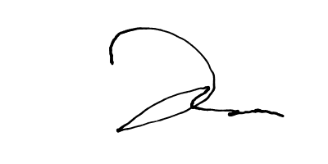
\includegraphics[height=1cm]{images/ttd-jazmy.png}\\[0.1cm]
Jazmy Izzati Alamsyah \\
NIM: 18221124
\chapter*{ABSTRAK}
\addcontentsline{toc}{chapter}{ABSTRAK}

\begin{center}

    \textbf{\MakeUppercase{Pengembangan Sistem Pemantauan Sampah Berbasis \protect\textit{Internet of Things} sebagai Dasar Analisis Pola Pembuangan Sampah}} \\
    \vspace{0.4cm}
    oleh \\
    \vspace{0.4cm}
    Jazmy Izzati Alamsyah\\
    18221124\\
\end{center}


\begin{spacing}{1.0}
Pengelolaan sampah di lingkungan kampus menghadapi tantangan berupa kurangnya data terstruktur mengenai pola pembuangan sampah, sehingga menyulitkan pengambilan keputusan berbasis data dalam jadwal pengangkutan dan alokasi sumber daya. Penelitian ini mengembangkan sistem pemantauan sampah berbasis \textit{Internet of Things} (IoT) yang mampu mengotomasi pengumpulan data pembuangan sampah di Gedung Labtek VIII Institut Teknologi Bandung, khususnya pada area depan Laboratorium IoT Lantai 4, sebagai dasar bagi analisis pola pembuangan sampah. Sistem dirancang menggunakan arsitektur IoT 4-\textit{layer} yang terdiri dari \textit{Perception Layer} (mikrokontroler ESP32, sensor jarak VL53L0X, sensor arus INA219, dan modul GSM SIM800L), \textit{Network Layer} berbasis protokol MQTT, \textit{Middleware Layer} menggunakan Node-RED untuk pemrosesan aliran data, serta \textit{Application Layer} dengan basis data Supabase dan \textit{dashboard} Next.js untuk visualisasi data. Selama periode observasi 37 hari, tiga unit perangkat sensor berhasil mengumpulkan 816 \textit{records} data dengan tingkat keberhasilan pengiriman sebesar 91,9\%, dengan 805 \textit{records} dinyatakan valid setelah \textit{filtering} data kotor. Analisis deskriptif yang dilakukan terhadap data tersebut mengidentifikasi empat pola pembuangan sampah, yang terdiri dari tiga pola temporal dan satu pola komposisi, yaitu pola \textit{peak hour} yang konsisten pada pukul 14:00--17:00 (29,6\% dari total \textit{event} penambahan), pola konsentrasi aktivitas pada jam kerja (07:00--19:00) di hari kerja, pola pengaruh hari libur berupa penurunan aktivitas pembuangan, serta pola dominasi sampah anorganik yang menyumbang 13 dari 27 \textit{event} penambahan (48,1\% dari total \textit{event}) dengan kontribusi volume sebesar 51,7\% dari total delta positif. Perangkat bawaan pihak ketiga diadaptasi melalui lima penyesuaian \textit{firmware}, dengan empat di antaranya terbukti efektif dalam meningkatkan reliabilitas dan konsistensi pengukuran. Seluruh 10 kebutuhan fungsional dan 7 dari 8 kebutuhan nonfungsional sistem berhasil dipenuhi. Penelitian ini menunjukkan bahwa sistem pemantauan berbasis \textit{Internet of Things} (IoT) dapat menjadi dasar yang andal untuk menghasilkan wawasan terstruktur dalam mendukung pengelolaan sampah kampus.

Kata kunci: \textit{smart waste bin}, \textit{Internet of Things}, ESP32, VL53L0X, MQTT, pola pembuangan sampah, analisis temporal.
\end{spacing}
\chapter*{KATA PENGANTAR}
\addcontentsline{toc}{chapter}{KATA PENGANTAR}

Puji syukur penulis panjatkan ke hadirat Tuhan Yang Maha Esa atas segala rahmat dan karunia-Nya sehingga Laporan Tugas Akhir yang berjudul ``Pengembangan Sistem \textit{Smart Waste Bin} Berbasis \textit{Internet of Things} untuk Analisis Pola Pembuangan Sampah'' ini dapat diselesaikan dengan baik. Laporan ini disusun sebagai salah satu syarat kelulusan tingkat sarjana pada Program Studi Sistem dan Teknologi Informasi, Sekolah Teknik Elektro dan Informatika, Institut Teknologi Bandung.

Pada kesempatan ini, penulis ingin menyampaikan terima kasih kepada:

\begin{enumerate}
    \item Bapak Dr. Fadhil Hidayat, S.Kom., M.T. selaku Pembimbing I dan Bapak Dr. Ir. Arry Akhmad Arman, M.T. selaku Pembimbing II, yang telah memberikan bimbingan, arahan, serta masukan yang sangat berarti selama proses penelitian dan penulisan laporan ini berlangsung.

    \item Seluruh dosen dan staf Program Studi Sistem dan Teknologi Informasi ITB yang telah memberikan ilmu dan dukungan selama masa perkuliahan.

    \item Keluarga tercinta, Bapak, Ibu, dan 3 Adik saya yang senantiasa memberikan doa, dukungan, dan semangat tanpa henti selama penulis menempuh pendidikan hingga menyelesaikan Tugas Akhir ini.

    \item Teman-teman, baik yang menemani secara langsung maupun daring, yang turut memberikan dukungan dan semangat selama penulisan Tugas Akhir ini.

    \item Mas Fryma dan Mas Farhan dari PT Layanan Cerdas Indonesia, yang telah memberikan dukungan teknis dan membantu dalam proses \textit{maintenance} perangkat selama penelitian berlangsung.

    \item Seluruh pihak yang tidak dapat disebutkan satu per satu yang telah turut membantu penyelesaian Tugas Akhir ini.
\end{enumerate}

\begin{flushright}
    Bandung, 5 Maret 2026\\[1cm]
    Penulis\\[1cm]
    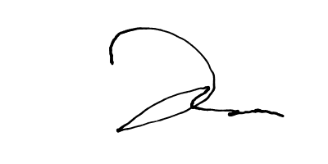
\includegraphics[height=1.5cm]{images/ttd-jazmy.png}\\[0.2cm]
    Jazmy Izzati Alamsyah
\end{flushright}

% --- \newgeometry{twoside} di-comment untuk menghilangkan blank page ---
% --- Uncomment hanya jika dokumen akan dicetak bolak-balik (duplex) ---
% \newgeometry{twoside, a4paper, inner=4cm, outer=3cm, top=3cm, bottom=3cm}

\input{7 Daftar Isi.tex}
\input{8 Daftar Gambar.tex}
\cleardoublepage
\renewcommand{\cftlottitlefont}{\hfill\large\bfseries\MakeUppercase}
\renewcommand{\cftafterlottitle}{\hfill}
\titlespacing*{\chapter}{0pt}{40pt}{20pt}
\phantomsection
\addcontentsline{toc}{chapter}{DAFTAR TABEL}
\setlength{\cfttabnumwidth}{3.5em}
\renewcommand{\cfttabaftersnum}{\hspace{0.5em}}
\listoftables

\input{10 Daftar Persamaan.tex}
% \input{11 Daftar Algoritma.tex}  % tidak digunakan
\input{12 Daftar Listing.tex}
\cleardoublepage
\begin{center}
{\fontsize{14}{16.8}\selectfont\textbf{DAFTAR SIMBOL}}\\[1em]
\end{center}
\label{chap:simbol}
\addcontentsline{toc}{chapter}{DAFTAR SIMBOL}
\vspace{2em}

\begin{longtable}{@{} l >{\raggedright\arraybackslash}p{8cm} c @{}}
\multicolumn{1}{l}{\textbf{Notasi}} &
\multicolumn{1}{l}{\textbf{Deskripsi}} &
\multicolumn{1}{l}{\parbox[c]{3cm}{\raggedright\textbf{Pertama digunakan (hal.)}}} \\[0.5ex]
\hline
\endhead

% ─── Simbol Matematika Umum ───────────────────────────────
\multicolumn{3}{@{}l}{\textbf{Simbol Matematika}} \\[0.5ex]

$\Delta$   & Delta: selisih atau perubahan nilai & \pageref{eq:fill-level} \\
$\pm$      & Plus-minus: toleransi atau rentang nilai & \pageref{eq:battery-percent} \\
$\%$       & Persentase & \pageref{eq:fill-level} \\
$\times$   & Operator perkalian & \pageref{eq:fill-level} \\
$\leq$     & Kurang dari atau sama dengan & \pageref{sec:perancangan-dashboard} \\
$\geq$     & Lebih dari atau sama dengan & \pageref{sec:perancangan-firmware} \\
$\approx$  & Mendekati & \pageref{tab:statistik-interval} \\[1ex]

% ─── Variabel Pengukuran Sensor ───────────────────────────
\multicolumn{3}{@{}l}{\textbf{Variabel Pengukuran Sensor}} \\[0.5ex]

$d$        & Jarak terukur sensor VL53L0X (mm) & \pageref{eq:fill-level} \\
$d_{max}$  & Kedalaman \textit{bin} atau jarak maksimum sensor (mm) & \pageref{eq:fill-level} \\
$F$        & Tingkat kepenuhan \textit{bin} (\textit{fillLevel}, \%) & \pageref{eq:fill-level} \\
$V$        & Tegangan baterai perangkat (Volt) & \pageref{eq:battery-percent} \\
$I$        & Arus baterai perangkat (mA) & \pageref{tab:fungsi-komponen} \\
$P$        & Daya terpakai perangkat (mW) & \pageref{tab:fungsi-komponen} \\
$B$        & Persentase baterai (\textit{Battery Percent}, \%) & \pageref{eq:battery-percent} \\[1ex]

% ─── Statistik Deskriptif ─────────────────────────────────
\multicolumn{3}{@{}l}{\textbf{Statistik Deskriptif}} \\[0.5ex]

$n$        & Jumlah sampel atau \textit{records} data & \pageref{tab:statistik-filllevel} \\
$\bar{x}$  & Rata-rata (\textit{mean}) & \pageref{tab:statistik-filllevel} \\
$\tilde{x}$ & Median & \pageref{tab:statistik-filllevel} \\
$\sigma$   & Deviasi standar (\textit{standard deviation}) & \pageref{tab:statistik-filllevel} \\
$x_{min}$  & Nilai minimum & \pageref{tab:statistik-filllevel} \\
$x_{max}$  & Nilai maksimum & \pageref{tab:statistik-filllevel} \\[1ex]

% ─── Notasi Sistem IoT ────────────────────────────────────
\multicolumn{3}{@{}l}{\textbf{Notasi Sistem IoT}} \\[0.5ex]

$t$        & Waktu atau \textit{timestamp} & \pageref{tab:dfd-alur} \\
$\Delta t$ & Selisih waktu atau interval antar pengiriman data & \pageref{tab:statistik-interval} \\
$QoS$      & \textit{Quality of Service} protokol MQTT (level 0, 1, atau 2) & \pageref{sec:perancangan-middleware} \\
$CR$       & \textit{Consistency Ratio} pada metode AHP & \pageref{tab:bobot-kriteria} \\
$CI$       & \textit{Consistency Index} pada metode AHP & \pageref{tab:bobot-kriteria} \\
$RI$       & \textit{Random Index} pada metode AHP & \pageref{tab:bobot-kriteria} \\
$\lambda_{max}$ & Nilai eigen terbesar (\textit{maximum eigenvalue}) pada AHP & \pageref{tab:bobot-kriteria} \\[1ex]

% ─── Satuan ───────────────────────────────────────────────
\multicolumn{3}{@{}l}{\textbf{Satuan}} \\[0.5ex]

mm         & Milimeter (satuan panjang jarak sensor) & \pageref{eq:fill-level} \\
V          & Volt (satuan tegangan listrik) & \pageref{eq:battery-percent} \\
mA         & Miliampere (satuan arus listrik) & \pageref{tab:hasil-ina219} \\
mW         & Miliwatt (satuan daya listrik) & \pageref{tab:hasil-ina219} \\
mAh        & Miliampere-jam (satuan kapasitas baterai) & \pageref{tab:pemilihan-teknologi} \\
ms         & Milidetik (satuan waktu) & \pageref{tab:hasil-nodered} \\

\end{longtable}
\cleardoublepage
\begin{center}
{\fontsize{14}{16.8}\selectfont\textbf{DAFTAR SINGKATAN}}\\[1em]
\end{center}
\label{chap:singkatan}
\addcontentsline{toc}{chapter}{DAFTAR SINGKATAN}
\vspace{2em}

\begin{longtable}{@{} l >{\raggedright\arraybackslash}p{8cm} c @{}}
\multicolumn{1}{l}{\textbf{Singkatan}} &
\multicolumn{1}{l}{\textbf{Deskripsi}} &
\multicolumn{1}{l}{\parbox[c]{3cm}{\raggedright\textbf{Pertama digunakan (hal.)}}} \\[0.5ex]
\hline
\endhead

AHP    & \textit{Analytical Hierarchy Process}                    & \pageref{sec:analisis-solusi} \\
API    & \textit{Application Programming Interface}               & \pageref{sec:perancangan-dashboard} \\
APN    & \textit{Access Point Name}                               & \pageref{tab:hasil-gprs} \\
BLE    & \textit{Bluetooth Low Energy}                            & \pageref{tab:perbandingan-mcu} \\
BaaS   & \textit{Backend as a Service}                            & \pageref{sec:perancangan-database} \\
CI     & \textit{Consistency Index}                               & \pageref{tab:bobot-kriteria} \\
CR     & \textit{Consistency Ratio}                               & \pageref{tab:bobot-kriteria} \\
CRUD   & \textit{Create, Read, Update, Delete}                    & \pageref{sec:impl-dashboard} \\
CSS    & \textit{Cascading Style Sheets}                          & \pageref{tab:teknologi-dashboard} \\
DFD    & \textit{Data Flow Diagram}                               & \pageref{sec:gambaran-umum} \\
GPRS   & \textit{General Packet Radio Service}                    & \pageref{tab:konfigurasi-lingkungan} \\
GPIO   & \textit{General Purpose Input/Output}                    & \pageref{sec:perancangan-firmware} \\
GSM    & \textit{Global System for Mobile Communications}         & \pageref{tab:konfigurasi-lingkungan} \\
HTTP   & \textit{Hypertext Transfer Protocol}                     & \pageref{sec:studi-protokol} \\
HTTPS  & \textit{Hypertext Transfer Protocol Secure}              & \pageref{sec:studi-protokol} \\
I2C    & \textit{Inter-Integrated Circuit}                        & \pageref{tab:pemilihan-teknologi} \\
IoT    & \textit{Internet of Things}                              & \pageref{chap:pendahuluan} \\
ITB    & Institut Teknologi Bandung                               & \pageref{chap:pendahuluan} \\
ITU    & \textit{International Telecommunication Union}           & \pageref{chap:studi-literatur} \\
JSON   & \textit{JavaScript Object Notation}                      & \pageref{tab:payload-data} \\
KF     & Kebutuhan Fungsional                                     & \pageref{tab:kebutuhan-fungsional} \\
KNF    & Kebutuhan Nonfungsional                                  & \pageref{tab:kebutuhan-nonfungsional} \\
LCI    & Layanan Cerdas Indonesia                                 & \pageref{chap:pendahuluan} \\
MQTT   & \textit{Message Queuing Telemetry Transport}             & \pageref{chap:studi-literatur} \\
NB-IoT & \textit{Narrowband Internet of Things}                   & \pageref{chap:studi-literatur} \\
ORM    & \textit{Object-Relational Mapping}                       & \pageref{tab:teknologi-dashboard} \\
PCB    & \textit{Printed Circuit Board}                           & \pageref{sec:diskusi-evaluasi} \\
QoS    & \textit{Quality of Service}                              & \pageref{sec:perancangan-middleware} \\
RAM    & \textit{Random Access Memory}                            & \pageref{tab:perbandingan-mcu} \\
REST   & \textit{Representational State Transfer}                 & \pageref{sec:perancangan-database} \\
RI     & \textit{Random Index}                                    & \pageref{tab:bobot-kriteria} \\
RM     & Rumusan Masalah                                          & \pageref{sec:analisis-kebutuhan} \\
SDGs   & \textit{Sustainable Development Goals}                   & \pageref{chap:studi-literatur} \\
SE     & Skenario Evaluasi                                        & \pageref{sec:metode-evaluasi} \\
SIM    & \textit{Subscriber Identity Module}                      & \pageref{tab:pemilihan-teknologi} \\
SoC    & \textit{State of Charge}                                 & \pageref{sec:perancangan-iot} \\
SQL    & \textit{Structured Query Language}                       & \pageref{sec:perancangan-database} \\
SWB    & \textit{Smart Waste Bin}                                 & \pageref{sec:analisis-solusi} \\
TCP    & \textit{Transmission Control Protocol}                   & \pageref{chap:studi-literatur} \\
ToF    & \textit{Time-of-Flight}                                  & \pageref{chap:studi-literatur} \\
UAT    & \textit{User Acceptance Testing}                         & \pageref{chap:pendahuluan} \\
UDP    & \textit{User Datagram Protocol}                          & \pageref{chap:studi-literatur} \\
UI     & \textit{User Interface}                                  & \pageref{tab:hasil-ui} \\
UART   & \textit{Universal Asynchronous Receiver-Transmitter}     & \pageref{tab:perbandingan-mcu} \\
URL    & \textit{Uniform Resource Locator}                        & \pageref{tab:tautan-penting} \\

\end{longtable}

% ==========================================
% MAINMATTER
% ==========================================
\mainmatter
\addtocontents{toc}{\protect\setlength{\cftbeforechapskip}{10pt}}
\addtocontents{toc}{\protect\renewcommand{\protect\cftchapfont}{\protect\bfseries}}
\addtocontents{toc}{\protect\renewcommand{\protect\cftchappagefont}{\protect\bfseries}}
\renewcommand{\cftchapleader}{\bfseries\cftdotfill{\cftchapdotsep}}

\cleardoublepage
\chapter{PENDAHULUAN}
\label{chap:pendahuluan}

% --- Latar Belakang ---
\section{Latar Belakang}

Pertumbuhan populasi global dan urbanisasi yang pesat telah meningkatkan volume produksi sampah secara signifikan. Menurut World Bank, produksi sampah global diproyeksikan mencapai 3,4 miliar ton pada tahun 2050, meningkat dari 2,01 miliar ton pada tahun 2016 \autocite{kaza2018}.
Peningkatan volume sampah ini menimbulkan tantangan kompleks dalam pengelolaan limbah yang efisien dan berkelanjutan.

Salah satu tantangan utama dalam pengelolaan sampah adalah ketiadaan data terstruktur mengenai pola pembuangan. Pertanyaan seperti kapan terjadi puncak pembuangan, apakah ada perbedaan pola antara hari kerja dan akhir pekan, serta jenis sampah apa yang mendominasi, menjadi sulit dijawab tanpa sistem \textit{monitoring} yang memadai. Metode konvensional seperti pengecekan visual atau pencatatan manual memiliki keterbatasan dalam hal konsistensi, akurasi, dan cakupan waktu, sehingga pengambilan keputusan sering dilakukan tanpa basis data.

Perkembangan teknologi \textit{Internet of Things} (IoT) membuka peluang untuk mengatasi permasalahan tersebut. Sensor yang dipasang pada tempat sampah dapat memantau tingkat kepenuhan secara periodik, menyimpan data ke basis data, dan menghasilkan \textit{insight} mengenai pola pembuangan. Di Indonesia, salah satu contoh perangkat \textit{Smart Waste Bin} yang telah dikembangkan adalah produk dari PT Layanan Cerdas Indonesia (LCI), yang telah diimplementasikan di beberapa kota untuk pemantauan kapasitas kontainer sampah \autocite{LCI2024}. Namun, perangkat \textit{Smart Waste Bin} yang tersedia secara komersial umumnya dirancang untuk skala perkotaan, sehingga konfigurasi perangkat termasuk \textit{firmware} belum tentu sesuai untuk lingkungan yang lebih kecil seperti kampus, di mana dinamika pembuangan sampah berubah dalam hitungan jam dan memerlukan resolusi data yang lebih tinggi.

Berdasarkan permasalahan tersebut, penelitian ini bertujuan untuk mengembangkan sistem \textit{Smart Waste Bin} berbasis IoT yang disesuaikan dengan kebutuhan lingkungan kampus, baik dari sisi perangkat lunak sistem maupun \textit{firmware} perangkat. Sistem yang dibangun kemudian diuji di Gedung Labtek VIII ITB untuk mengumpulkan data dan menganalisis pola pembuangan sampah yang dihasilkan.

% --- Rumusan Masalah ---
\section{Rumusan Masalah}

Berdasarkan latar belakang dan permasalahan di atas, penelitian ini merumuskan pertanyaan penelitian sebagai berikut:

\begin{enumerate}
    \item Bagaimana rancangan dan implementasi sistem \textit{Smart Waste Bin} berbasis IoT yang mampu mengumpulkan data pembuangan sampah secara periodik dan terstruktur?

    \item Pola pembuangan sampah apa yang dapat diidentifikasi berdasarkan data yang dikumpulkan oleh sistem, dan seberapa valid pola tersebut terhadap observasi lapangan?
\end{enumerate}

% --- Tujuan ---
\section{Tujuan}

Penelitian ini bertujuan untuk merancang dan mengimplementasikan sistem \textit{Smart Waste Bin} berbasis \textit{Internet of Things} untuk memahami pola pembuangan sampah di Gedung Labtek VIII ITB. Secara detil, tujuan penelitian ini adalah:

\begin{enumerate}
    \item Merancang arsitektur dan mengimplementasikan sistem \textit{Smart Waste Bin} berbasis IoT yang mampu mengumpulkan data pembuangan sampah secara periodik dan terstruktur.

    \item Mengidentifikasi pola pembuangan sampah berdasarkan data yang dikumpulkan oleh sistem dan memvalidasinya melalui observasi lapangan.
\end{enumerate}

% --- Batasan Masalah ---
\section{Batasan Masalah}

Penelitian ini memiliki batasan-batasan berikut:

\begin{enumerate}
    \item Pengujian lapangan dari sistem yang dibangun dilakukan di Lantai 4 area depan Laboratorium IoT, Gedung Labtek VIII Institut Teknologi Bandung.

    \item Sistem menggunakan 3 unit perangkat \textit{Smart Waste Bin} yang masing-masing ditempatkan berdasarkan jenis sampah: organik, anorganik, dan residu.

    \item Perangkat IoT yang digunakan merupakan modifikasi dari perangkat \textit{Smart Waste Bin} pihak ketiga yang disesuaikan untuk kebutuhan lingkungan kampus.

    \item Interval pengumpulan data ditetapkan $\pm$2,5 jam berdasarkan pertimbangan kapasitas daya baterai perangkat.

    \item Klasifikasi jenis sampah mengacu pada penempatan fisik tempat sampah (organik, anorganik, residu), bukan melalui sensor klasifikasi otomatis.

    \item Analisis pola pembuangan sampah mencakup pola temporal (distribusi jam dan hari), tren volume, serta komposisi jenis sampah berdasarkan data yang dikumpulkan sistem.
\end{enumerate}

% --- Metodologi ---
\section{Metodologi}

Pelaksanaan tugas akhir ini didukung oleh studi literatur dan menggunakan metodologi \textit{Design Science Research} (DSR) untuk pengembangan sistem. Studi literatur dilakukan untuk membangun fondasi teoritis dan memahami teknologi yang relevan, sedangkan DSR digunakan sebagai kerangka kerja pengembangan dan evaluasi artefak yang berfokus pada pemenuhan kebutuhan (\textit{requirement}) yang telah ditetapkan.

\subsection{Studi Literatur}

Studi literatur dilakukan untuk mengumpulkan informasi yang relevan tentang topik yang diangkat, mencakup teori, konsep, teknologi, dan penelitian terdahulu yang telah dilakukan oleh peneliti lain. Studi literatur ini menjadi fondasi dalam pengembangan sistem \textit{Smart Waste Bin} berbasis \textit{Internet of Things}.

Aktivitas yang dilakukan pada tahap studi literatur meliputi:

\begin{enumerate}
    \item \textbf{Pencarian Literatur}

    Melakukan pencarian literatur dari berbagai sumber akademik dan ilmiah, seperti jurnal internasional, konferensi, artikel ilmiah, buku, dan dokumentasi teknis. Pencarian dilakukan menggunakan basis data akademik seperti IEEE \textit{Xplore}, \textit{Google Scholar}, \textit{ScienceDirect}, dan \textit{Springer}. Kata kunci yang digunakan dalam pencarian mencakup: ``\textit{smart waste bin}'', ``IoT \textit{waste management}'', ``\textit{waste pattern analysis}'', ``\textit{smart waste monitoring}'', ``\textit{sensor-based waste management}'', dan kombinasi kata kunci lainnya yang relevan.

    \item \textbf{Pengelompokan Literatur}

    Literatur yang diperoleh dikelompokkan berdasarkan kategori-kategori seperti konsep dan teori dasar tentang \textit{Internet of Things} (IoT), teknologi sensor dan perangkat keras untuk \textit{monitoring} sampah, arsitektur sistem dan integrasi IoT, penelitian terdahulu tentang \textit{smart waste bin} dan pengelolaan sampah berbasis teknologi, dan metode analisis data temporal.

    \item \textbf{Penapisan dan Evaluasi Literatur}

    Literatur yang telah dikumpulkan disaring berdasarkan relevansi, kualitas publikasi, dan kebaruan informasi.

    \item \textbf{Sintesis dan Dokumentasi}

    Hasil studi literatur disintesis untuk mengidentifikasi \textit{gap} penelitian, \textit{best practices}, dan pendekatan yang dapat diadopsi atau dikembangkan lebih lanjut. Seluruh proses studi literatur didokumentasikan dan hasil sintesisnya akan dijelaskan secara sistematis di Bab II Studi Literatur.
\end{enumerate}

\subsection{Metodologi \textit{Design Science Research}}

Pengembangan sistem \textit{Smart Waste Bin} menggunakan metodologi \textit{Design Science Research} (DSR) sebagaimana dirumuskan oleh Peffers dkk. \autocite{peffers2007}. Metodologi ini dipilih karena penelitian ini berorientasi pada pembangunan dan evaluasi sebuah artefak, yaitu sistem \textit{Smart Waste Bin}, bukan pada riset perilaku pengguna. DSR menyediakan kerangka kerja yang sistematis dan teruji untuk penelitian yang menghasilkan artefak teknologi, dengan validasi yang difokuskan pada pemenuhan kebutuhan (\textit{requirement}) yang telah ditetapkan. DSR mencakup enam fase utama, yaitu identifikasi masalah dan motivasi, definisi tujuan solusi, perancangan dan pengembangan, demonstrasi, evaluasi, dan komunikasi. Berikut adalah penjelasan untuk setiap fase yang diterapkan secara spesifik pada penelitian ini:

\begin{enumerate}
    \item \textbf{Identifikasi Masalah dan Motivasi}

    Fase ini bertujuan untuk mengidentifikasi permasalahan yang melatarbelakangi penelitian beserta motivasinya. Aktivitas pada fase ini meliputi:
    \begin{enumerate}[a.]
        \item Mengidentifikasi permasalahan pengelolaan sampah yang masih bergantung pada penjadwalan tetap tanpa mempertimbangkan kondisi aktual kepenuhan tempat sampah, serta ketiadaan data dan informasi kondisi sampah yang terstruktur.
        \item Melakukan pengamatan langsung terhadap kondisi sistem pembuangan yang ada untuk memperkuat pemahaman terhadap permasalahan.
    \end{enumerate}

    \item \textbf{Definisi Tujuan Solusi}

    Fase ini bertujuan untuk merumuskan tujuan solusi berdasarkan permasalahan yang telah diidentifikasi, yang dinyatakan dalam bentuk kebutuhan sistem. Aktivitas pada fase ini meliputi:
    \begin{enumerate}[a.]
        \item Mengolah hasil identifikasi masalah untuk merumuskan \textit{gap} dan kebutuhan akan sistem pengumpulan data yang terstruktur.
        \item Merumuskan spesifikasi kebutuhan sistem, yang mencakup pendefinisian Kebutuhan Fungsional (pengumpulan data, penyimpanan, dan visualisasi pola) serta Kebutuhan Nonfungsional (performa dan reliabilitas). Spesifikasi kebutuhan inilah yang menjadi acuan utama dalam perancangan dan evaluasi.
    \end{enumerate}

    \item \textbf{Perancangan dan Pengembangan}

    Fase ini bertujuan untuk merancang dan membangun artefak sistem \textit{Smart Waste Bin} berdasarkan kebutuhan yang telah ditetapkan. Aktivitas pada fase ini meliputi:
    \begin{enumerate}[a.]
        \item Mengeksplorasi berbagai alternatif arsitektur dan solusi teknologi, serta memilih alternatif terbaik menggunakan metode pengambilan keputusan yang terukur berdasarkan kriteria kelayakan teknis, kesesuaian tujuan, waktu, dan biaya.
        \item Merancang dan mengimplementasikan adaptasi pada sisi \textit{firmware} perangkat keras bawaan untuk menyesuaikannya dengan karakteristik lingkungan kampus dan mengoptimalkan keandalan operasional.
        \item Mengembangkan sistem penerimaan, transmisi, dan penyimpanan data pembuangan sampah sesuai dengan arsitektur yang terpilih.
        \item Mengintegrasikan seluruh komponen perangkat keras dan perangkat lunak sehingga membentuk satu kesatuan sistem yang dapat beroperasi secara otomatis.
    \end{enumerate}

    \item \textbf{Demonstrasi}

    Fase ini bertujuan untuk menunjukkan bahwa artefak yang telah dibangun dapat digunakan untuk menyelesaikan permasalahan, melalui penerapan di lapangan. Aktivitas pada fase ini meliputi:
    \begin{enumerate}[a.]
        \item Menempatkan unit \textit{smart waste bin} pada lokasi yang telah ditentukan untuk mengumpulkan data pembuangan sampah dalam periode tertentu.
        \item Melakukan \textit{monitoring} terhadap operasional sistem selama periode pengumpulan data untuk memastikan sistem merekam dan mentransmisikan data dengan konsisten.
    \end{enumerate}

    \item \textbf{Evaluasi}

    Fase ini bertujuan untuk mengukur seberapa baik artefak memenuhi kebutuhan yang telah ditetapkan pada fase definisi tujuan. Aktivitas pada fase ini meliputi:
    \begin{enumerate}[a.]
        \item Mengevaluasi pemenuhan Kebutuhan Fungsional dan Nonfungsional sistem berdasarkan data hasil demonstrasi.
        \item Menganalisis data yang terkumpul menggunakan analisis statistik deskriptif dan analisis temporal untuk memahami pola pembuangan sampah di lokasi penelitian.
        \item Mengevaluasi efektivitas adaptasi \textit{firmware} yang telah dikembangkan terhadap keandalan dan kualitas data sistem.
    \end{enumerate}

    \item \textbf{Komunikasi}

    Fase ini bertujuan untuk mengomunikasikan permasalahan, artefak yang dihasilkan, dan hasil evaluasinya. Aktivitas pada fase ini berupa penyusunan dokumentasi penelitian secara sistematis dalam bentuk laporan tugas akhir, yang mencakup seluruh proses mulai dari identifikasi masalah hingga kesimpulan.
    \vfill
\end{enumerate}

% --- Sistematika Penulisan ---
\section{Sistematika Penulisan}

Laporan tugas akhir ini disusun dengan sistematika penulisan sebagai berikut:

\begin{enumerate}
    \item Bab I Pendahuluan: Berisi latar belakang, rumusan masalah, tujuan, batasan masalah, metodologi, dan sistematika penulisan laporan tugas akhir.

    \item Bab II Studi Literatur: Berisi kajian pustaka yang relevan dengan topik tugas akhir, mencakup teori dan konsep dasar \textit{Internet of Things}, teknologi sensor dan perangkat keras untuk \textit{monitoring} sampah, arsitektur sistem IoT, serta penelitian terdahulu yang berkaitan dengan \textit{smart waste bin} dan pengelolaan sampah berbasis teknologi.

    \item Bab III Analisis: Berisi penjelasan tentang analisis kebutuhan pengguna dan sistem, termasuk pendefinisian kebutuhan fungsional dan nonfungsional sistem \textit{Smart Waste Bin}.

    \item Bab IV Perancangan: Berisi penjelasan tentang perancangan solusi yang diusulkan, mencakup arsitektur sistem IoT 4-\textit{layer}, perancangan perangkat keras, perangkat lunak, dan \textit{firmware}.

    \item Bab V Implementasi: Berisi penjelasan tentang proses implementasi sistem, termasuk pengembangan \textit{firmware}, integrasi komponen, dan pengembangan \textit{dashboard} visualisasi data.

    \item Bab VI Evaluasi: Berisi analisis dan evaluasi terhadap sistem yang diimplementasikan, mencakup pengujian kebutuhan fungsional dan nonfungsional, analisis pola pembuangan sampah, serta evaluasi peningkatan \textit{firmware}.

    \item Bab VII Kesimpulan dan Saran: Berisi kesimpulan dari hasil pelaksanaan tugas akhir dan saran untuk pengembangan lebih lanjut.

    \item Daftar Pustaka: Berisi daftar referensi yang digunakan dalam penyusunan laporan tugas akhir.

    \item Lampiran: Berisi dokumen-dokumen pendukung seperti data lengkap hasil pengujian dan dokumentasi lapangan.
\end{enumerate}
\cleardoublepage
\chapter{STUDI LITERATUR}
\label{chap:studi-literatur}

Bab ini menyajikan hasil studi literatur sebagaimana ditetapkan pada Subbab I.5.1. Studi literatur dilakukan untuk membangun fondasi teoritis yang mendasari perancangan dan implementasi sistem \textit{Smart Waste Bin} berbasis IoT. Pembahasan mencakup tiga topik utama: pengelolaan sampah dan tantangannya dalam konteks lingkungan kampus, teknologi \textit{Internet of Things} beserta arsitektur dan komponen yang relevan, serta studi terkait sistem \textit{Smart Waste Bin} yang telah dikembangkan sebelumnya.

% ============================================================
\section{Pengelolaan Sampah}
% ============================================================

Pengelolaan sampah merupakan kegiatan sistematis yang mencakup pengumpulan, pengangkutan, pemrosesan, daur ulang, dan pembuangan material sampah yang dihasilkan dari aktivitas manusia. Pengelolaan sampah yang efektif harus mempertimbangkan aspek teknis, ekonomi, lingkungan, dan sosial untuk mencapai tujuan keberlanjutan \autocite{giurea2024}. Sistem pengelolaan sampah yang baik tidak hanya berfokus pada pembuangan akhir, tetapi juga pada pengurangan volume sampah dari sumbernya, pemilahan, dan pemanfaatan kembali material yang masih memiliki nilai.

\subsection{Konsep Dasar Pengelolaan Sampah}

Dalam konteks hierarki pengelolaan sampah, terdapat beberapa tingkatan prioritas yang harus dipertimbangkan berdasarkan \textit{Waste Framework Directive}. Tingkatan tertinggi adalah pencegahan dan pengurangan sampah di sumber (\textit{waste prevention and reduction}), diikuti oleh persiapan untuk penggunaan kembali (\textit{preparing for reuse}), daur ulang (\textit{recycling}), pemulihan energi (\textit{energy recovery}), dan terakhir adalah pembuangan akhir (\textit{disposal}) \autocite{ec2008}. Pendekatan hierarkis ini menekankan pentingnya upaya preventif dan pemanfaatan nilai ekonomi dari sampah sebelum melakukan pembuangan.

Pengelolaan sampah modern juga menerapkan prinsip \textit{circular economy} yang bertujuan untuk meminimalkan limbah dan memaksimalkan pemanfaatan sumber daya melalui sistem yang tertutup. \textit{Circular economy} didefinisikan sebagai sistem regeneratif di mana \textit{input} sumber daya, limbah, emisi, dan kebocoran energi diminimalkan melalui strategi memperlambat, menutup, dan mempersempit aliran material dan energi \autocite{geissdoerfer2017}. Dalam konteks institusi pendidikan tinggi, penerapan \textit{circular economy} mencakup tiga dimensi keberlanjutan: ekonomi, ekologi, dan sosial, yang bekerja secara sinergis untuk menciptakan sistem pengelolaan sampah yang tidak hanya ramah lingkungan, tetapi juga bertanggung jawab secara ekonomi dan sosial \autocite{giurea2024}.

\textit{Sustainable Development Goals} (SDGs) yang ditetapkan oleh \textit{United Nations} juga menekankan pentingnya pengelolaan sampah berkelanjutan sebagai bagian dari upaya mencapai dunia yang lebih berkelanjutan dan berkeadilan pada tahun 2030 \autocite{un2015}. Pengelolaan sampah yang efektif berkontribusi pada beberapa SDGs, termasuk kota dan komunitas berkelanjutan (SDG 11), konsumsi dan produksi yang bertanggung jawab (SDG 12), serta aksi iklim (SDG 13).

\subsection{Tantangan Pengelolaan Sampah pada Lingkungan Kampus}

Lingkungan kampus dan gedung perkuliahan memiliki karakteristik unik dalam hal pengelolaan sampah yang membedakannya dari lingkungan perkotaan pada umumnya. Institusi pendidikan tinggi menghadapi tantangan khusus karena kepadatan populasi yang tinggi, variasi aktivitas yang beragam, dan pola penggunaan yang dinamis sepanjang hari dan minggu \autocite{bahcelioglu2020}. Karakteristik ini menyebabkan volume dan komposisi sampah yang dihasilkan sangat bervariasi tergantung pada waktu, aktivitas akademik, dan kegiatan yang berlangsung di gedung.

Berdasarkan \textit{review} komprehensif terhadap penelitian tentang pengelolaan sampah di institusi pendidikan tinggi, rata-rata tingkat produksi sampah adalah $0{,}19 \pm 0{,}21$ kg/hari per orang (median $0{,}093$ kg/hari per orang) \autocite{rodriguez2024}. Komposisi sampah didominasi oleh sampah organik yang mencapai rata-rata $30 \pm 19$\% dari total sampah, diikuti oleh kertas dan kardus ($23 \pm 13$\%), dan plastik ($18 \pm 11$\%) \autocite{bahcelioglu2020}.

Salah satu tantangan utama adalah keterbatasan data mengenai pola pembuangan sampah. Penelitian menunjukkan bahwa sebagian besar institusi pendidikan mengalami kesulitan dalam melacak kapan, di mana, dan berapa banyak sampah yang dihasilkan karena tidak memiliki sistem \textit{monitoring} yang memadai \autocite{bahcelioglu2020}. Tanpa data yang \textit{reliable}, pengambilan keputusan terkait pengelolaan sampah menjadi tidak akurat, menghambat perencanaan strategis yang efektif, dan mempersulit pelacakan \textit{progress} terhadap tujuan pengurangan sampah \autocite{sensoneo2024}.

Tantangan lain yang dihadapi adalah variasi temporal dalam produksi sampah. Kampus dapat mengalami fluktuasi volume sampah yang signifikan antara periode aktif perkuliahan dan periode libur, dengan volume sampah dapat turun hingga sebagian kecil dari volume normal dalam waktu singkat \autocite{roadrunner2024}. Pola pembuangan sampah juga sangat dipengaruhi oleh jadwal perkuliahan, waktu istirahat, dan aktivitas khusus seperti seminar atau acara. Tanpa pemahaman yang baik terhadap pola temporal ini, alokasi sumber daya untuk pengumpulan sampah menjadi tidak efisien.

Tingkat partisipasi pengguna dalam pemilahan sampah juga menjadi tantangan tersendiri. Meskipun banyak kampus telah menyediakan fasilitas untuk pemilahan sampah, tingkat kepatuhan dan konsistensi dalam pemilahan masih rendah. Kontaminasi dalam aliran daur ulang terjadi ketika material yang tidak dapat didaur ulang tercampur dengan yang dapat didaur ulang, mengurangi efisiensi program daur ulang dan meningkatkan biaya pemrosesan \autocite{sensoneo2024}.

Tantangan operasional lainnya mencakup pengumpulan sampah yang tidak efisien, dengan \textit{pickup} yang sering dilakukan pada tempat sampah yang masih kosong atau sebagian terisi, mengakibatkan pemborosan bahan bakar, jam kerja, dan biaya pemeliharaan. Kondisi \textit{bin} yang meluap tidak hanya menciptakan lingkungan kampus yang tidak menarik, tetapi juga berkontribusi pada kontaminasi aliran daur ulang karena orang berhenti memilah sampah dan membuangnya ke \textit{bin} kosong terdekat tanpa memperhatikan jenis \textit{bin} tersebut \autocite{sensoneo2024}.

\subsection{Data dalam Pengelolaan Sampah}

Data merupakan fondasi penting dalam pengambilan keputusan untuk pengelolaan sampah yang efektif dan efisien. Sistem pengelolaan sampah berbasis data memungkinkan identifikasi pola, prediksi kebutuhan, dan optimalisasi operasional yang tidak dapat dicapai melalui pendekatan konvensional. Dengan data yang akurat dan terstruktur, pengelola dapat memahami karakteristik sampah yang dihasilkan, mengidentifikasi area atau waktu yang memerlukan perhatian khusus, dan merancang strategi pengelolaan yang lebih responsif.

Keputusan yang diambil berdasarkan data sampah yang tidak \textit{reliable} dapat mengganggu akurasi pelaporan keberlanjutan dan menghambat perencanaan strategis yang efektif. Tanpa data yang dapat diandalkan, sulit untuk melacak kemajuan terhadap tujuan pengurangan sampah, mengidentifikasi inefisiensi, atau mengoptimalkan jadwal pengumpulan \autocite{sensoneo2024}.

Pemanfaatan teknologi sensor ultrasonik, \textit{Time-of-Flight} (ToF), dan perangkat IoT lainnya memungkinkan \textit{monitoring} \textit{bin} secara \textit{real-time}, yang dapat memberikan \textit{alert} ketika \textit{bin} mendekati atau mencapai kapasitas penuh \autocite{pires2025}. Sistem ini tidak hanya meningkatkan efisiensi operasional, tetapi juga mencegah kondisi \textit{bin} yang meluap yang dapat menciptakan risiko kesehatan dan lingkungan.

Selain itu, data pembuangan sampah dapat memberikan \textit{insight} berharga untuk pengembangan program edukasi dan perubahan perilaku. Dengan memahami kapan dan di mana sampah paling banyak dihasilkan, serta jenis sampah yang dominan, institusi dapat merancang intervensi yang lebih spesifik untuk mengurangi produksi sampah atau meningkatkan tingkat daur ulang. Dalam konteks institusi pendidikan tinggi, data pengelolaan sampah juga berkontribusi pada pelaporan keberlanjutan (\textit{sustainability reporting}) yang semakin menjadi standar dalam akreditasi dan \textit{ranking} universitas internasional \autocite{bahcelioglu2020}.

% ============================================================
\section{\textit{Internet of Things}}
% ============================================================

\textit{Internet of Things} (IoT) didefinisikan sebagai konsep yang menghubungkan benda fisik dan virtual melalui jaringan internet untuk memungkinkan pertukaran data secara otomatis. Kevin Ashton, yang pertama kali memperkenalkan istilah IoT pada tahun 1999, menjelaskan bahwa IoT memungkinkan komputer untuk secara mandiri mengumpulkan informasi tanpa bantuan manusia, sehingga dapat mengurangi pemborosan, biaya, serta meningkatkan efisiensi \autocite{ashton2009}.

IoT dapat dipahami sebagai keberadaan pervasif dari berbagai objek yang mampu berinteraksi dan bekerja sama satu sama lain melalui skema pengalamatan yang unik untuk mencapai tujuan bersama \autocite{atzori2010}. \textit{International Telecommunication Union} (ITU-T) mendefinisikan IoT sebagai infrastruktur global yang mendukung layanan canggih melalui konektivitas benda fisik dan virtual menggunakan teknologi informasi dan komunikasi yang terus berkembang \autocite{itu2012}. Sementara itu, IoT \textit{European Research Cluster} (IERC) mendefinisikan IoT sebagai infrastruktur jaringan global yang dinamis dengan kemampuan konfigurasi mandiri, menggunakan protokol komunikasi standar dan interoperabel \autocite{iotec2014}.

Dengan berbagai definisi tersebut, IoT secara umum dapat dipahami sebagai infrastruktur global yang menghubungkan benda fisik dan virtual melalui jaringan internet, memungkinkan pertukaran data secara otomatis tanpa intervensi manusia yang signifikan. IoT memberikan manfaat signifikan dalam berbagai sektor seperti transportasi, kesehatan, manufaktur, dan kota pintar.

\subsection{Arsitektur \textit{Internet of Things}}

Arsitektur IoT bertujuan untuk menciptakan sinergi antara berbagai sistem yang memungkinkan perangkat-perangkat IoT untuk berkomunikasi dan saling beroperasi secara otomatis. Salah satu model arsitektur IoT yang paling fundamental dan banyak diadopsi adalah model tiga \textit{layer} yang terdiri dari \textit{Perception Layer}, \textit{Network Layer}, dan \textit{Application Layer} \autocite{sethi2017}. Model ini menyediakan kerangka dasar untuk memahami bagaimana komponen-komponen IoT berinteraksi dari tingkat perangkat fisik hingga aplikasi pengguna akhir.

\begin{figure}[H]
  \caption{IoT Reference Model 3 \textit{Layer} \autocite{sethi2017}}
  \label{fig:iot-3layer}
  \centering
  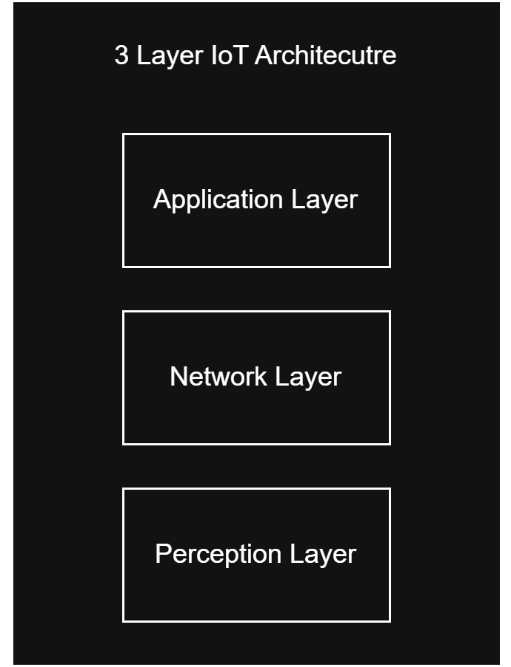
\includegraphics[width=0.5\textwidth]{images/iot-3layer.png}
  % RENAME: image5.png → iot-3layer.png di folder images/
\end{figure}

Berikut adalah penjelasan untuk setiap \textit{layer} pada arsitektur IoT berdasarkan Gambar \ref{fig:iot-3layer}:

\begin{enumerate}
  \item \textit{Perception Layer}

  \textit{Perception Layer}, yang juga dikenal sebagai \textit{Physical Layer} atau \textit{Device Layer}, merupakan lapisan paling bawah dalam arsitektur IoT. \textit{Layer} ini terdiri dari perangkat fisik seperti sensor, aktuator, \textit{RFID tags}, dan perangkat IoT lainnya yang berinteraksi langsung dengan lingkungan fisik \autocite{alfuqaha2015}. Fungsi utamanya adalah mengumpulkan data dari lingkungan sekitar, seperti suhu, kelembaban, tekanan, gerak, atau parameter lainnya sesuai dengan jenis sensor yang digunakan.

  Dalam konteks sistem \textit{Smart Waste Bin}, \textit{Perception Layer} mencakup sensor ultrasonik atau sensor \textit{Time-of-Flight} yang dipasang pada tempat sampah untuk mengukur tingkat kepenuhan secara periodik. Karakteristik penting dari \textit{layer} ini adalah kemampuannya untuk beroperasi dalam berbagai kondisi lingkungan, efisiensi energi untuk perangkat berbasis baterai, dan akurasi dalam pengukuran.

  \item \textit{Network Layer}

  \textit{Network Layer} berfungsi sebagai jembatan komunikasi yang menghubungkan \textit{Perception Layer} dengan \textit{Application Layer}. \textit{Layer} ini bertanggung jawab untuk transmisi data yang dikumpulkan oleh sensor ke sistem pemrosesan atau \textit{cloud server} \autocite{alfuqaha2015}. \textit{Network Layer} menggunakan berbagai protokol komunikasi dan teknologi jaringan seperti Wi-Fi, Ethernet, LoRaWAN, NB-IoT, Zigbee, Bluetooth, atau protokol lainnya tergantung pada kebutuhan jarak, \textit{bandwidth}, dan konsumsi energi.

  Dalam sistem \textit{Smart Waste Bin}, \textit{Network Layer} dapat menggunakan koneksi Wi-Fi atau \textit{cellular network} (seperti 4G/5G) untuk mengirimkan data tingkat kepenuhan sampah dari lokasi tempat sampah ke \textit{server} pusat secara periodik.

  \item \textit{Application Layer}

  \textit{Application Layer} merupakan lapisan tertinggi dalam arsitektur IoT yang berfungsi untuk menyediakan layanan dan antarmuka kepada pengguna akhir \autocite{alfuqaha2015}. \textit{Layer} ini mencakup aplikasi yang memproses, menganalisis, dan memvisualisasikan data yang diterima dari \textit{Network Layer}. Pada \textit{layer} ini terdapat sistem manajemen data, analitik, dan \textit{dashboard} yang memungkinkan pengguna untuk memantau kondisi, mengambil keputusan, atau melakukan kontrol terhadap perangkat IoT.

  Dalam konteks sistem \textit{Smart Waste Bin}, \textit{Application Layer} mencakup sistem \textit{database} untuk menyimpan data pembuangan sampah secara terstruktur, serta \textit{dashboard} yang memungkinkan pengelola untuk melihat status tempat sampah dan hasil analisis pola pembuangan.
\end{enumerate}

\subsection{Komponen Perangkat Keras pada IoT}

Implementasi sistem IoT memerlukan komponen \textit{hardware} yang berfungsi sebagai jembatan antara dunia fisik dan dunia digital. Komponen-komponen ini berada pada \textit{Perception Layer} dalam arsitektur IoT dan berperan dalam pengumpulan data dari lingkungan serta pemrosesan awal sebelum data dikirimkan ke sistem \textit{backend}.

\begin{enumerate}
  \item \textit{Microcontroller}

  \textit{Microcontroller} merupakan komputer kecil dalam satu \textit{chip} yang berfungsi sebagai ``otak'' dari perangkat IoT. \textit{Microcontroller} bertanggung jawab untuk membaca data dari sensor, memproses data tersebut, dan mengirimkannya ke \textit{server} atau \textit{cloud} melalui protokol komunikasi tertentu. Berbeda dengan mikroprosesor yang memerlukan komponen eksternal, \textit{microcontroller} mengintegrasikan semua komponen dalam satu \textit{chip}, termasuk \textit{CPU}, \textit{RAM}, \textit{ROM/Flash memory}, dan berbagai \textit{peripheral}.

  Tabel \ref{tab:perbandingan-mcu} menyajikan perbandingan empat \textit{platform microcontroller} yang umum digunakan dalam aplikasi IoT.

  \begin{table}[H]
    \caption{Perbandingan Arduino, Raspberry Pi, ESP8266 NodeMCU, dan ESP32 \autocite{ooko2019, espressif2021}}
    \label{tab:perbandingan-mcu}
    \begin{tabularx}{\textwidth}{| l | X | X | X | X |}
      \hline
      \textbf{Kriteria} & \textbf{Arduino} & \textbf{Raspberry Pi} & \textbf{ESP8266 NodeMCU} & \textbf{ESP32} \\
      \hline
      Pengembang & Arduino & Raspberry Pi Foundation & ESP8266 Open Source Community & Espressif Systems \\
      \hline
      Tipe & Single Board \textit{Microcontroller} & Mini Computer & Single Board \textit{Microcontroller} & Single Board \textit{Microcontroller} \\
      \hline
      Sistem Operasi & None & Linux & XTOS & FreeRTOS \\
      \hline
      CPU & Atmel, ARM & ARM Cortex & LXT106 & Dual-Core Xtensa 32-bit LX6 \\
      \hline
      Kecepatan \textit{Clock} & 16 MHz & 1,2 GHz & 26--52 MHz & 160--240 MHz \\
      \hline
      Memori & 32 KB & 1--4 GB & Hingga 128 MB & 520 KB SRAM \\
      \hline
      Penyimpanan & 1 KB & MicroSDHC & 4 MB \textit{Flash} & Hingga 16 MB \textit{Flash} \\
      \hline
      Tegangan Operasi & 5V & 5V & 3,3V & 3,3V \\
      \hline
      Konektivitas & I/O & SPI, I2C, UART, GPIO & UART, GPIO & UART, GPIO, Wi-Fi, BLE, SPI, I2C \\
      \hline
    \end{tabularx}
  \end{table}

  Arduino merupakan \textit{microcontroller} sederhana yang ideal untuk pengendalian perangkat keras dasar dengan kebutuhan komputasi ringan. ESP8266 NodeMCU dirancang khusus untuk aplikasi IoT yang memerlukan konektivitas jaringan dengan biaya rendah melalui Wi-Fi terintegrasi. ESP32 merupakan evolusi dari ESP8266 yang menawarkan peningkatan signifikan dalam hal performa, dilengkapi dengan prosesor \textit{dual-core} Xtensa 32-bit LX6 berkecepatan hingga 240 MHz, konektivitas Wi-Fi dan \textit{Bluetooth Low Energy} (BLE) secara simultan, serta dukungan sistem operasi FreeRTOS untuk pengelolaan \textit{multitasking} \autocite{espressif2021}. Raspberry Pi memiliki karakteristik yang lebih menyerupai komputer mini lengkap, cocok untuk aplikasi yang memerlukan pemrosesan data kompleks atau \textit{interfacing} dengan berbagai \textit{peripheral}, meskipun dengan konsumsi daya yang lebih tinggi.

  \item Sensor dan \textit{Actuator}

  Sensor adalah perangkat yang mendeteksi dan merespons \textit{input} dari lingkungan fisik, mengubah fenomena fisik seperti suhu, kelembaban, tekanan, cahaya, atau gerakan menjadi sinyal elektrik yang dapat diproses oleh \textit{microcontroller}. Sensor dapat dikategorikan sebagai sensor aktif yang memerlukan sumber daya eksternal, dan sensor pasif yang menghasilkan \textit{output} tanpa sumber daya eksternal. Dalam konteks IoT, sensor juga dikategorikan berdasarkan jenis data yang dihasilkan: sensor analog yang menghasilkan sinyal kontinu, dan sensor digital yang menghasilkan sinyal diskrit.

  \textit{Actuator}, di sisi lain, adalah perangkat yang melakukan aksi fisik berdasarkan perintah dari sistem kontrol, mengubah sinyal elektrik menjadi gerakan mekanis, panas, cahaya, atau bentuk energi lainnya. Dalam sistem IoT, \textit{actuator} memungkinkan sistem untuk tidak hanya mengamati lingkungan tetapi juga berinteraksi dan mengubah kondisi lingkungan berdasarkan data yang dikumpulkan.
\end{enumerate}

\subsection{Protokol Komunikasi IoT}

Protokol komunikasi dalam sistem IoT memainkan peran krusial dalam memastikan interoperabilitas dan efisiensi pertukaran data antar perangkat yang terhubung. Protokol-protokol ini dirancang untuk mengatasi tantangan spesifik yang dihadapi oleh perangkat IoT, seperti keterbatasan daya, \textit{bandwidth} terbatas, dan kebutuhan akan komunikasi yang andal dalam berbagai kondisi jaringan \autocite{alfuqaha2015}.

\begin{enumerate}
  \item HTTP/HTTPS (\textit{Hypertext Transfer Protocol})

  HTTP merupakan protokol komunikasi berbasis \textit{request-response} yang beroperasi di atas TCP (\textit{Transmission Control Protocol}). HTTPS adalah versi aman dari HTTP yang menggunakan enkripsi SSL/TLS untuk melindungi data selama transmisi. Kelebihan HTTP/HTTPS meliputi kompatibilitas yang luas dengan infrastruktur web yang ada dan kemudahan integrasi dengan layanan \textit{cloud}. Namun, HTTP memiliki \textit{overhead} yang relatif besar dibandingkan protokol IoT lainnya \autocite{alfuqaha2015}.

  \item MQTT (\textit{Message Queuing Telemetry Transport})

  MQTT adalah protokol \textit{messaging} berbasis \textit{publish-subscribe} yang dirancang khusus untuk perangkat dengan sumber daya terbatas dan jaringan dengan \textit{bandwidth} rendah atau tidak stabil. Protokol ini beroperasi di atas TCP dan menggunakan model \textit{broker} sentral yang mengelola komunikasi antara \textit{publisher} (perangkat yang mengirim data) dan \textit{subscriber} (aplikasi yang menerima data).

  Arsitektur \textit{publish-subscribe} MQTT memberikan beberapa keunggulan: \textit{decoupling} antara \textit{publisher} dan \textit{subscriber} yang memungkinkan skalabilitas lebih baik, dukungan tiga tingkat \textit{Quality of Service} (QoS 0, 1, dan 2), serta \textit{overhead} protokol yang sangat kecil dengan \textit{header} minimum hanya 2 \textit{bytes}. MQTT juga mendukung fitur \textit{retained messages} dan \textit{last will and testament} (LWT) yang menjadikannya sangat populer dalam aplikasi \textit{monitoring} dan telemetri IoT \autocite{alfuqaha2015}.

  \item CoAP (\textit{Constrained Application Protocol})

  CoAP adalah protokol aplikasi web yang dirancang khusus untuk perangkat terkendali (\textit{constrained devices}) dengan memori, daya pemrosesan, dan \textit{bandwidth} yang sangat terbatas. Berbeda dengan HTTP yang menggunakan TCP, CoAP beroperasi di atas UDP (\textit{User Datagram Protocol}), yang mengurangi \textit{overhead} komunikasi. CoAP cocok untuk aplikasi IoT yang memerlukan komunikasi \textit{RESTful} namun beroperasi pada perangkat dengan keterbatasan sumber daya yang signifikan \autocite{alfuqaha2015}.
\end{enumerate}

Pemilihan protokol komunikasi bergantung pada karakteristik perangkat, kebutuhan aplikasi, dan kondisi jaringan. HTTP/HTTPS cocok untuk sistem yang memerlukan integrasi mudah dengan infrastruktur web. MQTT ideal untuk aplikasi yang memerlukan komunikasi asinkron dengan \textit{overhead} rendah. CoAP merupakan pilihan terbaik untuk perangkat dengan keterbatasan sumber daya yang ekstrem.

% ============================================================
\section{Node-RED}
% ============================================================

Node-RED adalah \textit{platform} pemrograman visual berbasis aliran (\textit{flow-based}) yang dikembangkan oleh IBM dan kini merupakan proyek \textit{open-source} di bawah naungan OpenJS Foundation. \textit{Platform} ini dirancang untuk menghubungkan perangkat keras, API, dan layanan daring dengan cara yang mudah dipahami melalui antarmuka berbasis \textit{browser}. Node-RED berjalan di atas \textit{runtime} Node.js dan memungkinkan pengguna untuk membuat alur pemrosesan data dengan cara menyusun dan menghubungkan \textit{node}-\textit{node} fungsional tanpa harus menulis kode secara eksplisit \autocite{openjs2024}.

Konsep utama Node-RED adalah \textit{flow}, yaitu rangkaian \textit{node} yang saling terhubung melalui kabel (\textit{wire}). Terdapat tiga kategori \textit{node} utama: \textit{input node} sebagai sumber data (misalnya MQTT In, HTTP In), \textit{processing node} yang memanipulasi data (misalnya \textit{Function}, \textit{Switch}, \textit{Change}), serta \textit{output node} yang mengirimkan data ke tujuan akhir. Arsitektur ini menjadikan Node-RED sangat fleksibel sebagai komponen \textit{middleware} dalam ekosistem IoT, karena mampu menjembatani protokol komunikasi yang berbeda-beda \autocite{blackstock2016}.

Dalam konteks sistem IoT, Node-RED sering digunakan sebagai lapisan \textit{middleware} yang menerima data dari perangkat sensor melalui protokol MQTT atau HTTP, kemudian memvalidasi, mentransformasi, dan meneruskan data tersebut ke sistem penyimpanan atau layanan lainnya. Keunggulan Node-RED meliputi kemudahan konfigurasi melalui antarmuka visual, ekosistem \textit{node} yang kaya (tersedia lebih dari 4.000 \textit{node} tambahan di repositori publik), serta kemampuan \textit{deployment} yang cepat tanpa memerlukan proses kompilasi \autocite{clerissi2018}.

% ============================================================
\section{Studi Terkait}
% ============================================================

Bagian ini mengkaji penelitian-penelitian terdahulu yang relevan dengan topik pengembangan sistem \textit{Smart Waste Bin}, dengan fokus pada metode yang digunakan, hasil yang diperoleh, dan \textit{gap} yang menjadi dasar penelitian ini.

\subsection{Sistem \textit{Smart Waste Bin} Berbasis IoT}

\textcite{latifah2021} mengembangkan sistem \textit{Automated Trash Volume Monitoring} berbasis IoT untuk meningkatkan efisiensi pengelolaan sampah perkotaan. Sistem yang dikembangkan mengintegrasikan sensor ultrasonik HC-SR04 untuk \textit{monitoring} tingkat kepenuhan tempat sampah secara \textit{real-time}, mikrokontroler NodeMCU ESP8266 sebagai unit pemrosesan, dan \textit{platform} Blynk sebagai \textit{interface} untuk visualisasi dan notifikasi kepada petugas kebersihan. Sistem juga dilengkapi dengan servo motor yang mengoperasikan mekanisme pembukaan dan penutupan tutup tempat sampah secara otomatis ketika sensor infrared mendeteksi keberadaan pengguna pada jarak 50 cm.

Hasil pengujian sistem menunjukkan akurasi pengukuran volume sebesar 97\% dengan \textit{margin of error} 3\%, menunjukkan reliabilitas tinggi dalam \textit{monitoring} kondisi tempat sampah. Sistem berhasil mengirimkan notifikasi secara konsisten ketika \textit{threshold} tercapai, dengan \textit{average response time} kurang dari 5 detik dari deteksi hingga notifikasi diterima. Penelitian ini berkontribusi dalam demonstrasi \textit{feasibility} sistem IoT untuk \textit{waste management} dengan biaya implementasi yang relatif terjangkau.

\textcite{pires2025} mengembangkan sistem \textit{monitoring} urban berbasis IoT menggunakan teknologi sensor \textit{Time-of-Flight} (ToF) untuk pemantauan tingkat kepenuhan tempat sampah secara \textit{real-time}. Penelitian ini menggunakan sensor VL53L0X yang dipasang pada tempat sampah untuk mengukur jarak ke permukaan sampah dengan presisi tinggi, dikombinasikan dengan mikrokontroler yang dilengkapi konektivitas jaringan untuk transmisi data ke \textit{platform} pusat. Keunggulan utama pendekatan ini dibandingkan sensor ultrasonik konvensional adalah akurasi pengukuran yang lebih tinggi pada berbagai kondisi permukaan dan jenis material sampah.

Hasil penelitian menunjukkan bahwa sistem berbasis sensor ToF mampu memberikan akurasi pengukuran yang lebih konsisten dibandingkan sensor ultrasonik dalam kondisi penggunaan nyata. Data yang dikumpulkan selama periode evaluasi menunjukkan pola temporal yang jelas dalam pembuangan sampah, dengan \textit{peak} aktivitas yang berulang pada waktu-waktu tertentu. Penelitian ini memperkuat argumen bahwa sistem IoT berbasis data dapat menghasilkan \textit{insight} yang bernilai untuk optimalisasi pengelolaan sampah perkotaan.

Dibandingkan dengan kedua penelitian tersebut, penelitian ini memiliki perbedaan yang signifikan. Pertama, fokus utama bukan hanya pada \textit{monitoring} kepenuhan, tetapi pada analisis pola pembuangan sampah secara temporal untuk menghasilkan \textit{insight} yang dapat digunakan dalam pengambilan keputusan. Kedua, penelitian ini dilakukan pada lingkungan kampus dengan karakteristik yang berbeda dari lingkungan perkotaan umum, dan melibatkan optimasi \textit{firmware} perangkat pihak ketiga untuk menyesuaikan dengan kebutuhan lingkungan kampus. Ketiga, penelitian ini menggunakan arsitektur IoT 4-\textit{layer} yang lebih komprehensif dengan integrasi \textit{middleware} Node-RED, \textit{database} Supabase, dan \textit{dashboard} berbasis Next.js.
\cleardoublepage
\chapter{ANALISIS MASALAH}
\label{chap:analisis-masalah}

Bab ini merupakan pelaksanaan fase identifikasi masalah dan definisi tujuan solusi dari metodologi \textit{Design Science Research} yang telah ditetapkan pada Subbab I.5.2. Pada fase identifikasi masalah, dilakukan observasi langsung terhadap kondisi pengelolaan sampah di Gedung Labtek VIII ITB untuk memahami permasalahan yang dihadapi. Pada fase definisi tujuan solusi, hasil observasi dirumuskan menjadi kebutuhan sistem, baik fungsional maupun nonfungsional. Bab ini ditutup dengan pemilihan alternatif solusi menggunakan metode AHP, yang menjadi titik transisi menuju fase perancangan dan pengembangan pada Bab IV, karena penetapan alternatif solusi terpilih merupakan masukan utama bagi perancangan artefak.

Bab ini menguraikan tiga aspek. Pertama, analisis kondisi saat ini yang mengidentifikasi permasalahan pengelolaan sampah akibat tidak adanya data terstruktur mengenai pola pembuangan. Kedua, analisis kebutuhan yang merumuskan spesifikasi sistem berdasarkan permasalahan yang ditemukan. Ketiga, pemilihan solusi melalui evaluasi alternatif untuk menentukan pendekatan yang paling sesuai dengan tujuan penelitian.

% ============================================================
\section{Analisis Kondisi Saat Ini}
\label{sec:analisis-kondisi}
% ============================================================

Berdasarkan observasi yang dilakukan di Gedung Labtek VIII, kondisi pengelolaan sampah saat ini bersifat konvensional. Tempat sampah tidak dilengkapi sensor atau sistem \textit{monitoring}, pengecekan dilakukan secara visual oleh petugas kebersihan, dan pengumpulan sampah dilakukan berdasarkan jadwal tetap tanpa mempertimbangkan kondisi aktual kepenuhan.

Dari kondisi tersebut, teridentifikasi tiga permasalahan utama:

\begin{enumerate}
    \item \textbf{Ketiadaan Data Terstruktur Mengenai Pola Pembuangan Sampah}

    Sistem pengelolaan sampah saat ini tidak memiliki mekanisme untuk mengumpulkan data mengenai pola pembuangan. Tidak ada informasi mengenai kapan puncak pembuangan terjadi, apakah ada perbedaan pola antara hari kerja dan akhir pekan, atau jenis sampah apa yang mendominasi. Pengambilan keputusan dilakukan tanpa basis data yang memadai.

    \item \textbf{Tidak Ada Dokumentasi Data Historis}

    Sistem saat ini tidak mendokumentasikan data pembuangan sampah dalam format yang terstruktur. Akibatnya, analisis tren jangka panjang, identifikasi perubahan pola seiring waktu, dan evaluasi efektivitas strategi pengelolaan tidak dapat dilakukan.

    \item \textbf{Pengelolaan Berdasarkan Jadwal Tetap tanpa Umpan Balik Data}

    Pengumpulan sampah dilakukan berdasarkan jadwal tetap dan pengecekan visual secara manual tanpa mempertimbangkan kondisi aktual kepenuhan sebelum pengecekan. Pendekatan ini berpotensi menyebabkan inefisiensi, yaitu pengumpulan dilakukan terlalu cepat saat tempat sampah masih kosong atau terlambat saat sudah penuh.
\end{enumerate}

Di sisi lain, perangkat \textit{Smart Waste Bin} berbasis IoT yang tersedia secara komersial umumnya dirancang untuk skala perkotaan. Konfigurasi bawaan perangkat, termasuk interval pengiriman data dan mekanisme pembacaan sensor pada \textit{firmware}, belum tentu sesuai untuk lingkungan yang lebih kecil seperti kampus, yang dinamika pembuangan sampahnya berubah dalam hitungan jam dan memerlukan titik data yang lebih tinggi. Hal ini menunjukkan bahwa selain membangun sistem pengumpulan data, diperlukan juga penyesuaian pada sisi \textit{firmware} perangkat agar dapat beroperasi secara optimal di lingkungan kampus.

Permasalahan tersebut menunjukkan bahwa pengelolaan sampah di lokasi pengujian masih berfungsi untuk keperluan dasar, namun tidak dilengkapi kemampuan untuk mengumpulkan dan menganalisis data mengenai pola pembuangan sampah. Kebutuhan akan sistem pemantauan sampah berbasis \textit{Internet of Things} yang disesuaikan, baik dari sisi perangkat lunak maupun \textit{firmware}, menjadi dasar analisis kebutuhan pada subbab berikutnya.

% ============================================================
\section{Analisis Kebutuhan}
\label{sec:analisis-kebutuhan}
% ============================================================

Analisis kebutuhan terbagi menjadi tiga bagian utama. Pertama, identifikasi pengguna sistem untuk memahami \textit{stakeholder} yang terlibat dan ekspektasi mereka terhadap sistem. Kedua, perumusan kebutuhan fungsional yang mendeskripsikan fungsi-fungsi spesifik yang harus dimiliki sistem. Ketiga, spesifikasi kebutuhan nonfungsional yang mendefinisikan karakteristik kualitas sistem.

\subsection{Identifikasi Pemangku Kepentingan}

Sebagai dasar untuk merumuskan kebutuhan sistem, dilakukan identifikasi pemangku kepentingan (\textit{stakeholder}) yang terkait dengan sistem pemantauan sampah berbasis \textit{Internet of Things}. Identifikasi ini bertujuan untuk memetakan pihak-pihak yang berkepentingan terhadap keluaran sistem sehingga kebutuhan fungsional dan nonfungsional dapat diturunkan secara tepat. Perlu ditegaskan bahwa kebutuhan sistem pada penelitian ini diturunkan dari permasalahan yang telah diidentifikasi, bukan dari pengujian terhadap pengguna. Pemangku kepentingan yang teridentifikasi adalah sebagai berikut:

\begin{enumerate}
    \item \textbf{Pengurus Lantai/Pengelola Gedung}

    Pengelola gedung berkepentingan terhadap pengawasan pengelolaan sampah dan pengambilan keputusan terkait strategi pengelolaan. Keluaran sistem yang relevan bagi pengelola gedung adalah informasi mengenai pola pembuangan sampah, tren volume sampah, dan \textit{insight} yang dapat mendukung perencanaan dan optimalisasi pengelolaan sampah.

    \item \textbf{Peneliti/Pengembang Sistem}

    Peneliti berkepentingan terhadap pengembangan, implementasi, dan \textit{maintenance} sistem. Keluaran sistem yang relevan meliputi ketersediaan \textit{raw data} untuk analisis, kemampuan konfigurasi sistem (seperti interval pembacaan sensor atau \textit{threshold}), dan \textit{interface} untuk \textit{monitoring} status operasional sistem.

    \item \textbf{Pengguna Gedung (\textit{Indirect Stakeholder})}

    Meskipun pengguna gedung (mahasiswa, dosen, \textit{staff}) tidak berinteraksi langsung dengan sistem, mereka merupakan sumber data pembuangan sampah. Keberadaan \textit{smart waste bin} tidak boleh mengubah atau mempersulit proses pembuangan sampah yang sudah berjalan.
\end{enumerate}

\subsection{Kebutuhan Fungsional}

Kebutuhan fungsional menjelaskan fungsi-fungsi dan fitur-fitur yang harus tersedia pada sistem. Berdasarkan identifikasi masalah dan kebutuhan pengguna, kebutuhan fungsional sistem pemantauan sampah berbasis \textit{Internet of Things} disajikan pada Tabel \ref{tab:kebutuhan-fungsional}.

\begin{longtable}{| l | l | p{4cm} | p{5cm} |}
  \caption{Kebutuhan Fungsional}
  \label{tab:kebutuhan-fungsional} \\
    \hline
    \textbf{ID} & \textbf{Komponen} & \textbf{Kebutuhan} & \textbf{Penjelasan} \\
    \hline
  \endfirsthead
    \hline
    \textbf{ID} & \textbf{Komponen} & \textbf{Kebutuhan} & \textbf{Penjelasan} \\
    \hline
  \endhead
    \hline
  \endfoot
    KF-01 & IoT \textit{Device} & Pembacaan Sensor & Sistem harus dapat membaca tingkat kepenuhan \textit{waste bin} menggunakan sensor dengan interval yang ditentukan \\
    \hline
    KF-02 & IoT \textit{Device} & Transmisi Data & Sistem harus dapat mengirimkan data ke \textit{server} melalui protokol komunikasi secara otomatis \\
    \hline
    KF-03 & IoT \textit{Device} & \textit{Time Stamping} & Setiap data harus dilengkapi \textit{timestamp} dan identifier \textit{waste bin} \\
    \hline
    KF-04 & IoT \textit{Device} & Konversi Data & Sistem harus dapat mengkonversi jarak hasil pembacaan sensor menjadi persentase kepenuhan (0--100\%) \\
    \hline
    KF-05 & \textit{Database} & Penyimpanan Data & Sistem harus dapat menyimpan data sensor secara terstruktur dan historis \\
    \hline
    KF-06 & \textit{Database} & Pengambilan Data & Sistem dapat menyediakan \textit{query} untuk mengambil data secara spesifik \\
    \hline
    KF-07 & Analisis & Analisis Pola Temporal & Sistem harus dapat mengidentifikasi pola pembuangan berdasarkan waktu (\textit{hourly}, \textit{daily}, \textit{weekly}) \\
    \hline
    KF-08 & Analisis & Statistik Deskriptif & Sistem harus dapat menghasilkan statistik deskriptif (\textit{mean}, median, std) untuk setiap pola \\
    \hline
    KF-09 & \textit{Dashboard} & Visualisasi Data & \textit{Dashboard} harus menampilkan status kepenuhan \textit{waste bin} terbaru \\
    \hline
    KF-10 & \textit{Dashboard} & Grafik Pola Temporal & \textit{Dashboard} harus menampilkan grafik pola pembuangan per jam, per hari, dan per minggu \\
    \hline
\end{longtable}

Tabel \ref{tab:mapping-rm-kf} menyajikan \textit{mapping} setiap kebutuhan fungsional dengan rumusan masalah pada Bab I.

\begin{table}[H]
  \caption{\textit{Mapping} Rumusan Masalah dengan Kebutuhan Fungsional}
  \label{tab:mapping-rm-kf}
  \begin{tabularx}{\textwidth}{| X | l |}
    \hline
    \textbf{Rumusan Masalah} & \textbf{Kebutuhan Fungsional} \\
    \hline
    RM-1: Rancangan dan implementasi sistem pemantauan sampah berbasis \textit{Internet of Things} (IoT) yang mampu mengumpulkan data secara periodik dan terstruktur & KF-01, KF-02, KF-03, KF-04, KF-05, KF-06 \\
    \hline
    RM-2: Pola pembuangan sampah yang dapat diidentifikasi berdasarkan data sistem dan validasinya terhadap observasi lapangan & KF-07, KF-08, KF-09, KF-10 \\
    \hline
  \end{tabularx}
\end{table}

\subsection{Kebutuhan Nonfungsional}

Kebutuhan nonfungsional mendeskripsikan karakteristik kualitas sistem yang harus dipenuhi, mencakup aspek performa, keandalan, dan akurasi, sebagaimana disajikan pada Tabel \ref{tab:kebutuhan-nonfungsional}.

\begin{table}[H]
  \caption{Kebutuhan Nonfungsional}
  \label{tab:kebutuhan-nonfungsional}
  \begin{tabularx}{\textwidth}{| l | l | X | X |}
    \hline
    \textbf{ID} & \textbf{Kategori} & \textbf{Kebutuhan} & \textbf{Penjelasan} \\
    \hline
    KNF-01 & \textit{Performance} & Waktu Pembacaan Sensor & Sensor harus dapat melakukan pembacaan dalam waktu maksimal 1 menit \\
    \hline
    KNF-02 & \textit{Performance} & Latensi Transmisi Data & Data harus dikirim ke \textit{server} dalam waktu maksimal 10 detik setelah pembacaan \\
    \hline
    KNF-03 & \textit{Performance} & \textit{Response Time Dashboard} & \textit{Dashboard} harus merespons interaksi pengguna dalam waktu maksimal 3 detik \\
    \hline
    KNF-04 & \textit{Performance} & Waktu \textit{Query} & \textit{Query} data dari \textit{database} harus selesai dalam waktu maksimal 5 detik \\
    \hline
    KNF-05 & \textit{Reliability} & \textit{Uptime} Sistem IoT & Sistem IoT harus beroperasi dengan \textit{availability} minimal 95\% \\
    \hline
    KNF-06 & \textit{Reliability} & Konsistensi Pembacaan & Pembacaan setiap 3 jam dengan toleransi keterlambatan maksimal $\pm$15 menit \\
    \hline
    KNF-07 & \textit{Reliability} & Kelengkapan Data & Minimal 90\% data harus berhasil dikumpulkan selama periode penelitian \\
    \hline
    KNF-08 & \textit{Accuracy} & Akurasi Sensor & Pembacaan sensor harus memiliki galat maksimal 10\% dari volume aktual \\
    \hline
  \end{tabularx}
\end{table}

% ============================================================
\section{Analisis Pemilihan Solusi}
\label{sec:analisis-solusi}
% ============================================================

Berdasarkan analisis kondisi saat ini dan kebutuhan sistem yang telah diidentifikasi, terdapat beberapa alternatif pendekatan dalam pengembangan sistem pemantauan sampah berbasis \textit{Internet of Things} (IoT). Bagian ini menguraikan alternatif-alternatif solusi yang dapat diterapkan serta analisis pemilihan solusi menggunakan metode \textit{Analytical Hierarchy Process} (AHP).

\subsection{Alternatif Solusi}

Berdasarkan analisis kebutuhan, seluruh alternatif solusi menggunakan perangkat \textit{Smart Waste Bin} yang tersedia dari pihak ketiga sebagai basis perangkat keras. Perbedaan antar alternatif terletak pada pendekatan \textit{software stack} untuk pengumpulan data, \textit{monitoring}, dan kemudahan \textit{maintenance} sistem. Analisis pola pembuangan (KF-07, KF-08) pada seluruh alternatif dilakukan melalui \textit{pipeline} analisis data terpisah menggunakan \textit{script} pengolahan data. Perlu dicatat bahwa setiap alternatif yang dipertimbangkan harus mampu memenuhi seluruh kebutuhan fungsional yang telah ditetapkan, termasuk KF-09 (\textit{monitoring} data terkini) yang mensyaratkan keberadaan antarmuka \textit{dashboard}; oleh karena itu, pendekatan tanpa \textit{dashboard} tidak dimasukkan sebagai alternatif karena sejak awal bertentangan dengan kebutuhan fungsional.

Terdapat dua alternatif solusi yang dapat diimplementasikan:

\begin{enumerate}
    \item \textbf{Alternatif 1: Perangkat \textit{Smart Waste Bin} + \textit{Platform Cloud} (ThingSpeak/Blynk)}

    Menggunakan perangkat \textit{Smart Waste Bin} dan mengintegrasikannya dengan \textit{platform} IoT \textit{cloud} untuk penyimpanan data dan visualisasi. Karakteristik alternatif ini: \textit{platform cloud} menyediakan \textit{backend} dan \textit{dashboard} siap pakai, \textit{deployment} cepat dengan konfigurasi minimal, namun fitur analisis terbatas pada yang disediakan \textit{platform} dan terdapat keterbatasan dalam \textit{custom query} untuk analisis pola temporal yang kompleks.

    \item \textbf{Alternatif 2: Perangkat \textit{Smart Waste Bin} + \textit{Backend Custom} + \textit{Dashboard}}

    Menggunakan perangkat \textit{Smart Waste Bin}, mengembangkan \textit{middleware} dan \textit{backend custom} (Supabase PostgreSQL), serta membangun \textit{dashboard} untuk \textit{monitoring}. Karakteristik alternatif ini: \textit{backend custom} memungkinkan \textit{query} fleksibel untuk analisis pola temporal, \textit{dashboard custom} untuk \textit{monitoring} status terkini dan visualisasi historis, dapat diintegrasikan dengan sistem lain, namun memerlukan \textit{effort} pengembangan \textit{middleware} dan \textit{dashboard}.
\end{enumerate}

Tabel \ref{tab:pemenuhan-kf} menyajikan pemenuhan kebutuhan fungsional untuk setiap alternatif solusi.

\begin{table}[H]
  \caption{Pemenuhan Kebutuhan Fungsional per Alternatif}
  \label{tab:pemenuhan-kf}
  \begin{tabularx}{\textwidth}{| X | l | l |}
    \hline
    \textbf{Kebutuhan} & \textbf{Alt-1} & \textbf{Alt-2} \\
    \hline
    KF-01 s.d. KF-04 (IoT \textit{Device}) & Terpenuhi & Terpenuhi \\
    \hline
    KF-05, KF-06 (\textit{Database}) & Terbatas & Terpenuhi \\
    \hline
    KF-07, KF-08 (Analisis Pola) & Terbatas & Terpenuhi \\
    \hline
    KF-09 (\textit{Monitoring} Terkini) & Terpenuhi & Terpenuhi \\
    \hline
    KF-10 (Visualisasi Historis) & Terbatas & Terpenuhi \\
    \hline
  \end{tabularx}
\end{table}

\subsection{Analisis Penentuan Solusi Menggunakan Metode AHP}

Untuk menentukan alternatif solusi yang paling sesuai, digunakan metode \textit{Analytical Hierarchy Process} (AHP). Metode ini dipilih karena dapat mengakomodasi kriteria-kriteria dengan bobot yang berbeda serta memberikan hasil yang terukur dan terstruktur.

\begin{figure}[H]
  \caption{Struktur Hierarki AHP Pemilihan Solusi}
  \label{fig:kriteria-ahp}
  \centering
  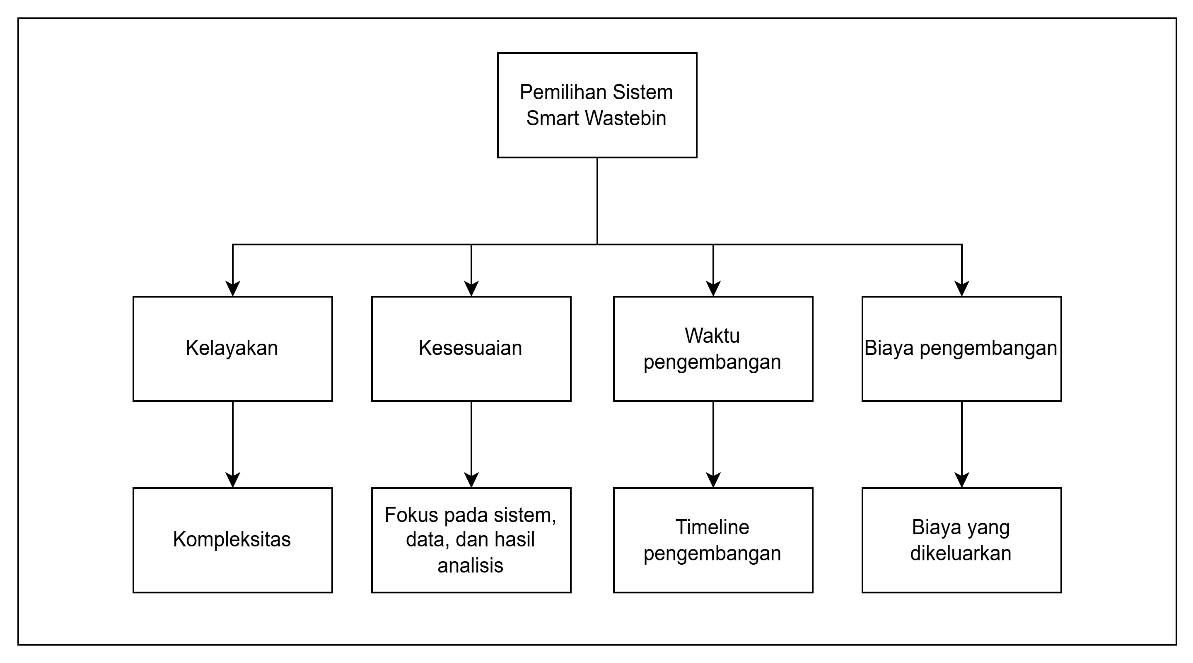
\includegraphics[width=0.9\textwidth]{images/kriteria-ahp.png}
  % RENAME: image6.png → kriteria-ahp.png di folder images/
\end{figure}

Gambar \ref{fig:kriteria-ahp} menunjukkan struktur hierarki AHP yang terdiri dari tujuan, kriteria, dan alternatif. Tabel \ref{tab:kriteria-ahp} menyajikan deskripsi setiap kriteria yang digunakan untuk evaluasi alternatif solusi.

\begin{table}[H]
  \caption{Kriteria Evaluasi Alternatif Solusi}
  \label{tab:kriteria-ahp}
  \begin{tabularx}{\textwidth}{| l | l | X |}
    \hline
    \textbf{ID} & \textbf{Kriteria} & \textbf{Deskripsi} \\
    \hline
    C-1 & Kelayakan Teknis & Kemudahan implementasi dengan kemampuan dan \textit{resource} yang tersedia \\
    \hline
    C-2 & Kesesuaian Tujuan & Seberapa baik solusi mendukung pencapaian tujuan penelitian (implementasi sistem, analisis pola, dan evaluasi \textit{firmware}) \\
    \hline
    C-3 & Waktu Pengembangan & Durasi waktu yang dibutuhkan untuk menyelesaikan pengembangan sistem \\
    \hline
    C-4 & Biaya & Total biaya implementasi yang dikeluarkan \\
    \hline
  \end{tabularx}
\end{table}

Penentuan bobot kriteria dilakukan melalui \textit{pairwise comparison matrix} menggunakan skala Saaty sebagaimana dijelaskan pada Subbab \ref{sec:ahp-teori}, dengan hasil disajikan pada Tabel \ref{tab:matriks-kriteria}. C-2 (Kesesuaian dengan tujuan penelitian) merupakan prioritas tertinggi karena sistem harus mendukung analisis pola dan evaluasi \textit{firmware}. C-1 (Kelayakan teknis) lebih penting dari C-3 (Waktu pengembangan). C-4 (Biaya) mendapat bobot terendah karena semua alternatif berada dalam \textit{range} biaya yang \textit{comparable}.

\begin{table}[H]
  \caption{Matriks Perbandingan Kriteria Berpasangan}
  \label{tab:matriks-kriteria}
  \begin{tabular}{| l | c | c | c | c |}
    \hline
    & \textbf{C-1} & \textbf{C-2} & \textbf{C-3} & \textbf{C-4} \\
    \hline
    \textbf{C-1} & 1     & 0,333 & 3     & 5 \\
    \hline
    \textbf{C-2} & 3     & 1     & 3     & 7 \\
    \hline
    \textbf{C-3} & 0,333 & 0,333 & 1     & 3 \\
    \hline
    \textbf{C-4} & 0,2   & 0,143 & 0,333 & 1 \\
    \hline
    \textbf{Jumlah} & 4,533 & 1,810 & 7,333 & 16 \\
    \hline
  \end{tabular}
\end{table}

Nilai perbandingan pada matriks menggunakan skala fundamental Saaty dengan nilai ganjil (1, 3, 5, 7, 9) yang merepresentasikan tingkat kepentingan: sama penting (1), sedikit lebih penting (3), lebih penting (5), sangat lebih penting (7), dan mutlak lebih penting (9), beserta nilai kebalikannya (resiprokal). Sebagai contoh, C-2 dinilai sedikit lebih penting dari C-1 (nilai 3) karena kesesuaian dengan tujuan penelitian merupakan prioritas tertinggi, sedangkan C-2 dinilai sangat lebih penting dari C-4 (nilai 7) karena seluruh alternatif memiliki struktur biaya yang serupa sehingga biaya bukan faktor pembeda yang signifikan.

Setelah proses normalisasi matriks dan perhitungan rata-rata baris, diperoleh bobot untuk setiap kriteria sebagaimana disajikan pada Tabel \ref{tab:bobot-kriteria}.

\begin{table}[H]
  \caption{Bobot Kriteria Hasil AHP}
  \label{tab:bobot-kriteria}
  \begin{tabular}{| l | c | c |}
    \hline
    \textbf{Kriteria} & \textbf{Bobot} & \textbf{Persentase} \\
    \hline
    C-1 (Kelayakan Teknis)   & 0,282 & 28,2\% \\
    \hline
    C-2 (Kesesuaian Tujuan)  & 0,515 & 51,5\% \\
    \hline
    C-3 (Waktu Pengembangan) & 0,145 & 14,5\% \\
    \hline
    C-4 (Biaya)              & 0,058 & 5,8\% \\
    \hline
  \end{tabular}
\end{table}

Nilai \textit{Consistency Ratio} (CR) dihitung untuk memastikan konsistensi penilaian. Dengan $\lambda_{max} = 4{,}141$, $CI = 0{,}047$, dan $RI = 0{,}90$, diperoleh $CR = 5{,}2\%$ yang berada di bawah batas 10\%, menunjukkan konsistensi yang baik.

\subsection{Evaluasi dan Pemilihan Alternatif Solusi}

Evaluasi dilakukan dengan membuat matriks perbandingan berpasangan untuk setiap kriteria terhadap kedua alternatif solusi. Tabel \ref{tab:justifikasi-kriteria} menyajikan justifikasi perbandingan untuk setiap kriteria.

\begin{table}[H]
  \caption{Justifikasi Perbandingan Alternatif pada Setiap Kriteria}
  \label{tab:justifikasi-kriteria}
  \begin{tabularx}{\textwidth}{| l | X |}
    \hline
    \textbf{Kriteria} & \textbf{Justifikasi Perbandingan} \\
    \hline
    C-1 (Kelayakan) & Alt-1 sedikit lebih unggul (nilai 3): \textit{platform} siap pakai dengan konfigurasi minimal, sedangkan Alt-2 memerlukan pengembangan \textit{middleware} dan \textit{dashboard} sendiri. \\
    \hline
    C-2 (Kesesuaian) & Alt-2 lebih unggul (nilai 5): memenuhi seluruh KF secara penuh, termasuk \textit{query} fleksibel untuk analisis pola temporal dan \textit{dashboard custom}; Alt-1 terbatas pada fitur analisis dan \textit{custom query} yang disediakan \textit{platform}. \\
    \hline
    C-3 (Waktu) & Alt-1 lebih unggul (nilai 5): \textit{plug-and-play} dengan waktu \textit{deployment} singkat, sedangkan Alt-2 memerlukan waktu pengembangan \textit{middleware} dan \textit{dashboard}. \\
    \hline
    C-4 (Biaya) & Setara (nilai 1): Alt-2 menggunakan layanan \textit{free tier} (Supabase, Vercel), sedangkan Alt-1 menggunakan \textit{platform} dengan \textit{tier} gratis yang tersedia; tidak ada perbedaan biaya yang signifikan. \\
    \hline
  \end{tabularx}
\end{table}

Karena perbandingan hanya melibatkan dua alternatif, setiap matriks perbandingan berukuran $2 \times 2$ yang secara matematis selalu konsisten ($CR = 0\%$). Tabel \ref{tab:bobot-lokal} menyajikan bobot lokal untuk setiap alternatif pada setiap kriteria hasil normalisasi matriks perbandingan berpasangan.

\begin{table}[H]
  \caption{Bobot Lokal Alternatif pada Setiap Kriteria}
  \label{tab:bobot-lokal}
  \begin{tabular}{| l | c | c | c | c |}
    \hline
    \textbf{Alternatif} & \textbf{C-1} & \textbf{C-2} & \textbf{C-3} & \textbf{C-4} \\
    \hline
    Alt-1: SWB + \textit{Platform Cloud}       & 0,750 & 0,167 & 0,833 & 0,500 \\
    \hline
    Alt-2: SWB + \textit{Backend} + \textit{Dashboard} & 0,250 & 0,833 & 0,167 & 0,500 \\
    \hline
  \end{tabular}
\end{table}

Skor global dihitung dengan mengalikan bobot lokal dengan bobot kriteria, sebagaimana disajikan pada Tabel \ref{tab:skor-global}.

\begin{table}[H]
  \caption{Skor Global untuk Setiap Alternatif Solusi}
  \label{tab:skor-global}
  \begin{tabularx}{\textwidth}{| X | l | c | c |}
    \hline
    \textbf{Alternatif} & \textbf{Perhitungan} & \textbf{Skor} & \textbf{\%} \\
    \hline
    Alt-1: SWB + \textit{Platform Cloud}       & $\Sigma(\text{bobot lokal} \times \text{bobot kriteria})$ & 0,447 & 44,7\% \\
    \hline
    Alt-2: SWB + \textit{Backend} + \textit{Dashboard} & $\Sigma(\text{bobot lokal} \times \text{bobot kriteria})$ & 0,553 & 55,3\% \\
    \hline
  \end{tabularx}
\end{table}

Berdasarkan Tabel \ref{tab:skor-global}, Alternatif 2 terpilih sebagai solusi terbaik dengan skor 0,553 (55,3\%), unggul dibandingkan Alternatif 1 (44,7\%). Keunggulan Alternatif 2 berasal dari dominasi pada kriteria C-2 (Kesesuaian dengan tujuan penelitian) yang memiliki bobot tertinggi (51,5\%), dengan kontribusi sebesar $0{,}833 \times 0{,}515 = 0{,}429$ terhadap skor globalnya. Meskipun Alternatif 1 unggul pada kelayakan teknis (C-1) dan waktu pengembangan (C-3), keterbatasan fitur analisis dan \textit{custom query} pada \textit{platform cloud} menyebabkan skor C-2 yang rendah, padahal kemampuan analisis pola temporal merupakan inti dari tujuan penelitian ini.

Dengan demikian, sistem pemantauan sampah berbasis \textit{Internet of Things} akan diimplementasikan menggunakan Alternatif 2, yaitu perangkat \textit{Smart Waste Bin} dari pihak ketiga dengan \textit{backend custom} (Supabase) dan \textit{dashboard} untuk \textit{monitoring}. Analisis pola pembuangan dilakukan melalui \textit{pipeline} analisis data terpisah. Selain pengembangan \textit{software stack}, adaptasi pada sisi \textit{firmware} perangkat juga akan dilakukan untuk menyesuaikan konfigurasi bawaan yang dirancang untuk skala perkotaan agar optimal di lingkungan kampus, sebagaimana telah diidentifikasi pada Subbab \ref{sec:analisis-kondisi}.
\cleardoublepage
\chapter{PERANCANGAN SISTEM \textit{SMART WASTE BIN}}
\label{chap:perancangan}

Bab ini merupakan bagian dari fase perancangan dan pengembangan dalam metodologi \textit{Design Science Research} yang telah diuraikan pada Subbab I.5.2. Berdasarkan hasil analisis kebutuhan dan pemilihan solusi pada Bab III, dirancang sistem pemantauan sampah berbasis \textit{Internet of Things} yang terdiri dari perangkat IoT, \textit{middleware}, \textit{database}, dan \textit{dashboard}.

Komponen sistem dibedakan menjadi dua kategori: komponen eksternal berupa perangkat IoT \textit{Smart Waste Bin} dari pihak ketiga, serta komponen internal yang dikembangkan oleh peneliti meliputi \textit{middleware}, \textit{database}, dan \textit{dashboard}. Karena konfigurasi \textit{firmware} bawaan perangkat dirancang untuk skala perkotaan sebagaimana diidentifikasi pada Subbab \ref{sec:analisis-kondisi}, bab ini juga menjelaskan perancangan adaptasi \textit{firmware} yang dilakukan agar perangkat dapat beroperasi optimal di lingkungan kampus.

% ============================================================
\section{Gambaran Umum Sistem}
\label{sec:gambaran-umum}
% ============================================================

Subbab ini menyajikan gambaran umum sistem pemantauan sampah berbasis \textit{Internet of Things} yang dikembangkan, mencakup arsitektur sistem secara keseluruhan, alur data dari pengumpulan hingga analisis, dan pemilihan teknologi. Gambaran umum ini bertujuan untuk memberikan pemahaman holistik mengenai struktur dan cara kerja sistem secara konseptual sebelum membahas perancangan detail pada subbab-subbab selanjutnya.

\subsection{Arsitektur Sistem}

Sistem Pemantauan Sampah Berbasis \textit{Internet of Things} dirancang menggunakan arsitektur berlapis (\textit{layered architecture}) yang mengacu pada model arsitektur IoT. Berbeda dengan model \textit{three-layer architecture} standar, sistem ini mengadopsi \textit{four-layer architecture} dengan penambahan \textit{Middleware Layer}. Pemilihan arsitektur empat \textit{layer} didasarkan pada kebutuhan untuk memisahkan fungsi transmisi data dengan fungsi pemrosesan dan \textit{routing} data, sehingga memberikan modularitas yang lebih baik dalam pengembangan dan pemeliharaan sistem.

Gambar \ref{fig:arsitektur-sistem} menunjukkan arsitektur keseluruhan sistem pemantauan sampah berbasis \textit{Internet of Things} yang terdiri dari empat \textit{layer} utama beserta pembagian komponen berdasarkan tanggung jawab pengembangan.

\begin{figure}[H]
  \caption{Arsitektur Sistem Pemantauan Sampah Berbasis \textit{Internet of Things}}
  \label{fig:arsitektur-sistem}
  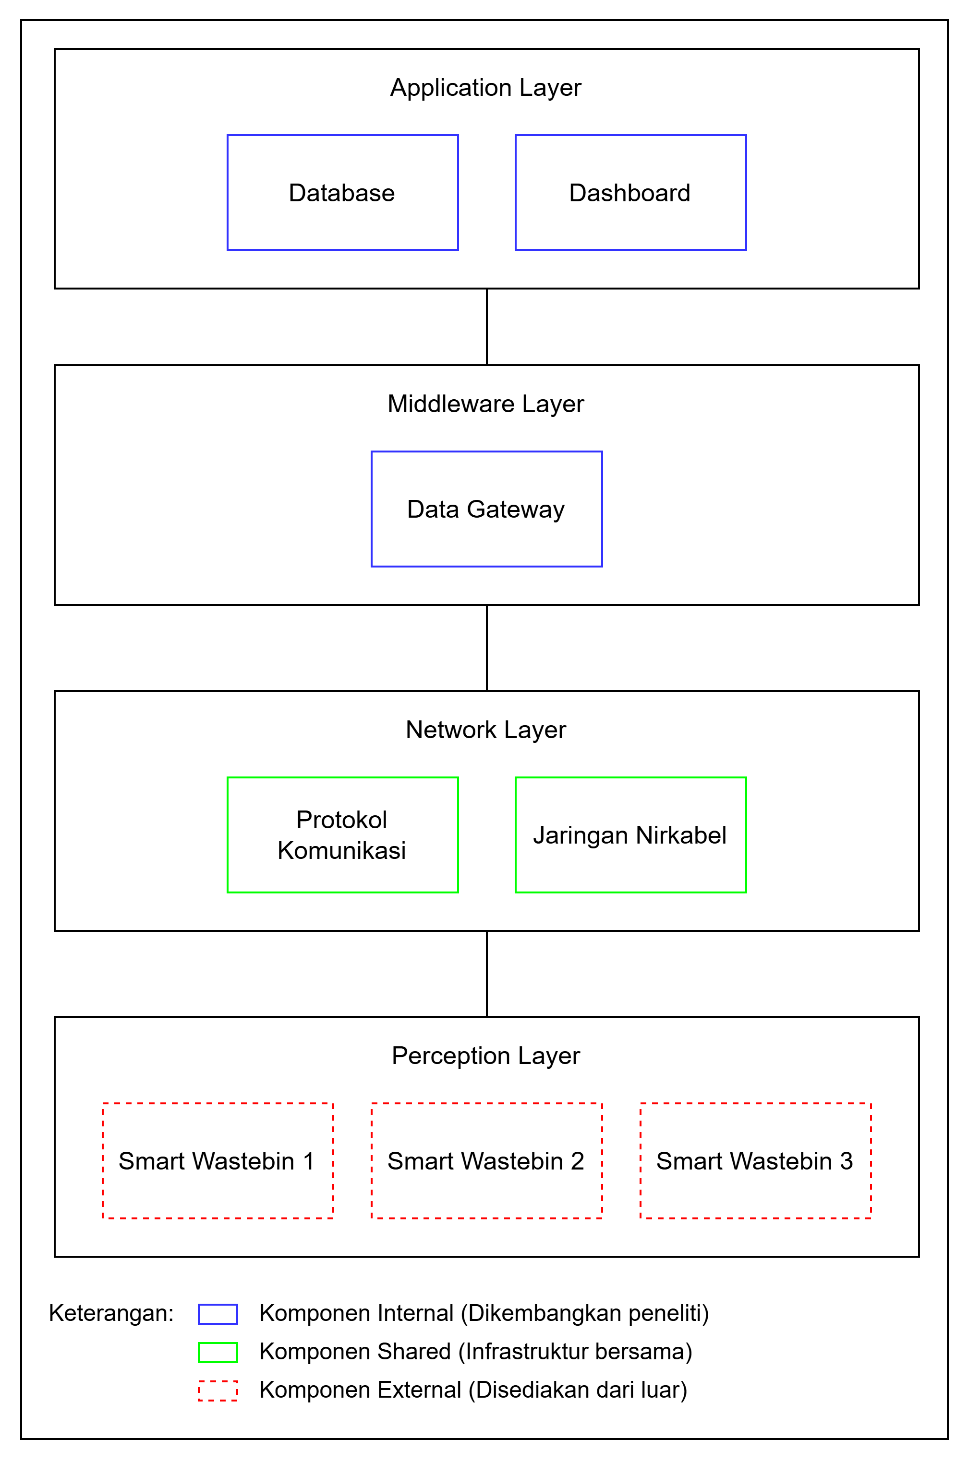
\includegraphics[width=0.7\textwidth]{images/arsitektur-sistem.png}
  % RENAME: image7.png → arsitektur-sistem.png
\end{figure}

Berdasarkan Gambar \ref{fig:arsitektur-sistem}, sistem terdiri dari empat \textit{layer} dengan fungsi sebagai berikut.

\begin{enumerate}
  \item \textit{Perception Layer}: terdiri dari tiga unit perangkat \textit{Smart Waste Bin} yang berfungsi mengumpulkan data tingkat kepenuhan tempat sampah secara periodik.
  \item \textit{Network Layer}: menyediakan infrastruktur komunikasi nirkabel untuk mentransmisikan data dari perangkat ke sistem penerima.
  \item \textit{Middleware Layer}: merupakan penambahan dari arsitektur standar, berfungsi sebagai data \textit{gateway} yang menerima, memvalidasi, dan meneruskan data ke \textit{layer} di atasnya.
  \item \textit{Application Layer}: terdiri dari dua komponen utama yaitu sistem \textit{database} untuk penyimpanan data dan \textit{dashboard} untuk visualisasi serta analisis pola pembuangan sampah.
\end{enumerate}

Arsitektur sistem juga membedakan komponen berdasarkan tanggung jawab pengembangan. Komponen eksternal mencakup perangkat IoT pada \textit{Perception Layer} yang disediakan oleh vendor. Komponen internal mencakup data \textit{gateway} pada \textit{Middleware Layer} serta seluruh komponen pada \textit{Application Layer} yang dikembangkan oleh peneliti. Komponen \textit{shared} mencakup infrastruktur \textit{Network Layer} yang digunakan bersama.

\subsection{Alur Data Sistem}

Sistem Pemantauan Sampah Berbasis \textit{Internet of Things} mengimplementasikan alur data yang terstruktur dari pengumpulan data di perangkat IoT hingga penyajian informasi kepada pengguna. Untuk menggambarkan alur data secara sistematis, digunakan \textit{Data Flow Diagram} (DFD) yang terdiri dari dua level: DFD Level 0 (\textit{Context Diagram}) dan DFD Level 1.

DFD Level 0 menggambarkan sistem pemantauan sampah berbasis \textit{Internet of Things} sebagai satu kesatuan proses yang berinteraksi dengan entitas eksternal, sebagaimana ditunjukkan pada Gambar \ref{fig:dfd-level0}.

\begin{figure}[H]
  \caption{\textit{Data Flow Diagram} Level 0}
  \label{fig:dfd-level0}
  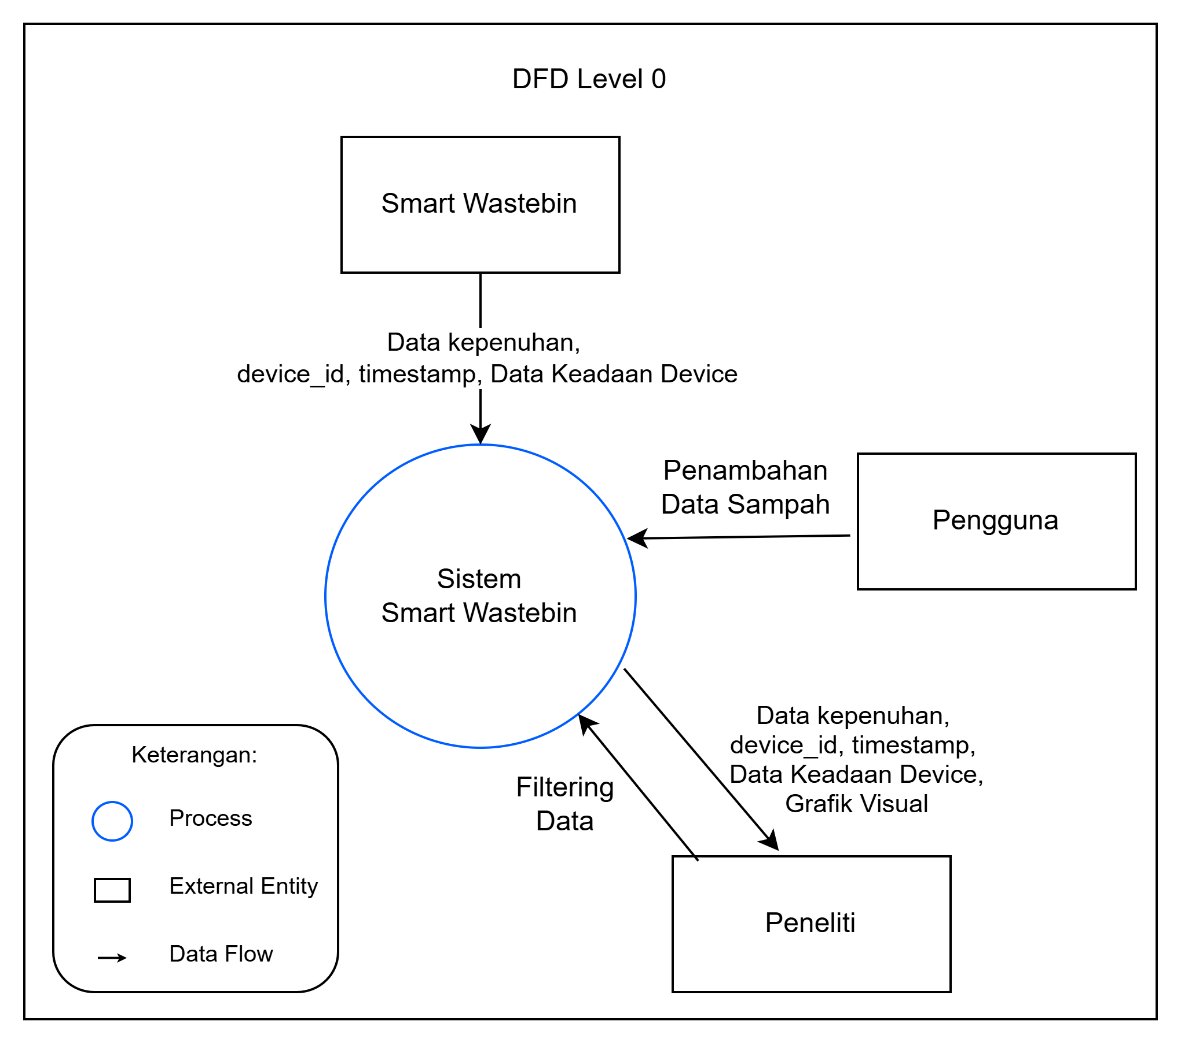
\includegraphics[width=0.85\textwidth]{images/dfd-level0.png}
  % RENAME: image8.png → dfd-level0.png
\end{figure}

Berdasarkan Gambar \ref{fig:dfd-level0}, terdapat dua entitas eksternal yang berinteraksi dengan sistem. Pertama, \textit{Smart Waste Bin} sebagai perangkat IoT sumber data yang mengirimkan data tingkat kepenuhan, identifier perangkat, dan \textit{timestamp} pembacaan secara periodik. Kedua, Pengguna yang mencakup pengelola gedung dan peneliti, yang mengirimkan \textit{request} data dan \textit{filter}, kemudian menerima visualisasi status dan grafik historis sebagai \textit{output}. Analisis pola terhadap data yang tersimpan dilakukan secara terpisah oleh peneliti, di luar alur operasional sistem.

DFD Level 1 menunjukkan dekomposisi proses tunggal pada DFD Level 0 menjadi tiga proses utama, sebagaimana ditunjukkan pada Gambar \ref{fig:dfd-level1}.

\begin{figure}[H]
  \caption{\textit{Data Flow Diagram} Level 1}
  \label{fig:dfd-level1}
  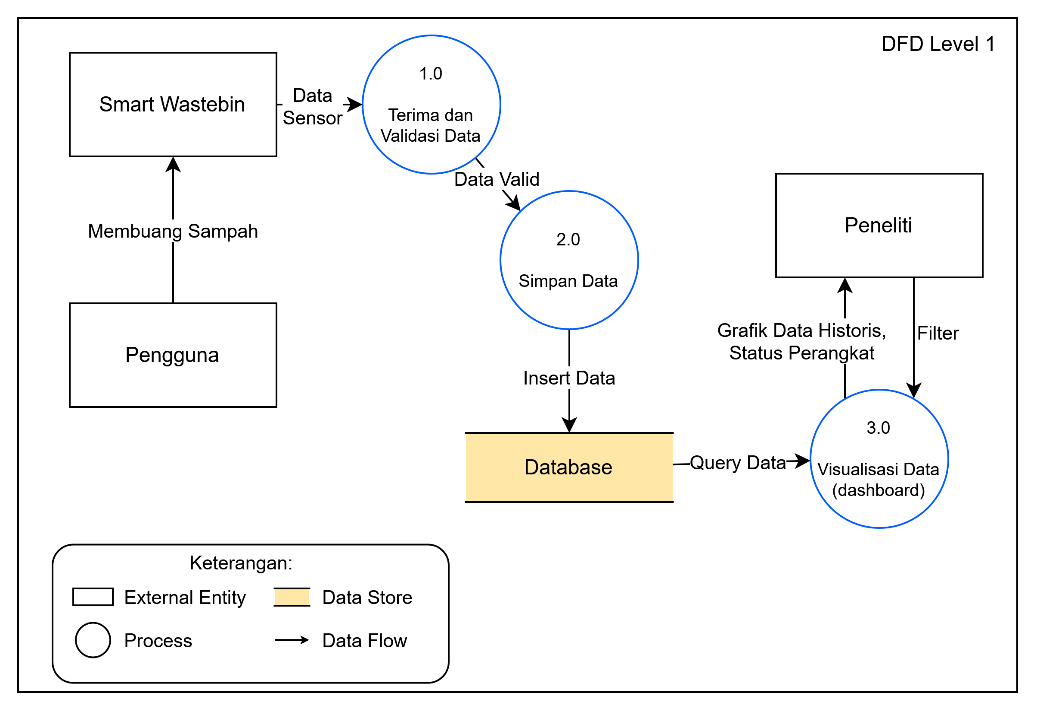
\includegraphics[width=0.85\textwidth]{images/dfd-level1.png}
  % RENAME: image9.png → dfd-level1.png
\end{figure}

Tabel \ref{tab:dfd-komponen} menyajikan deskripsi setiap komponen dalam DFD Level 1.

\begin{table}[H]
  \caption{Deskripsi Komponen DFD Level 1}
  \label{tab:dfd-komponen}
  \begin{tabularx}{\textwidth}{| l | l | l | X |}
    \hline
    \textbf{ID} & \textbf{Komponen} & \textbf{Tipe} & \textbf{Deskripsi} \\
    \hline
    1.0 & Terima \& Validasi Data & Proses & Menerima data dari perangkat IoT, melakukan \textit{parsing} dan validasi format serta nilai data \\
    \hline
    2.0 & Simpan Data & Proses & Menyimpan data yang telah tervalidasi ke dalam \textit{database} secara persisten melalui \textit{middleware} \\
    \hline
    3.0 & Visualisasi Data & Proses & Mengambil data dari \textit{database}, menyajikan dalam bentuk \textit{dashboard} dan grafik, serta memberikan status perangkat untuk kebutuhan pemeliharaan \\
    \hline
    D1 & \textit{Database} & Data Store & Menyimpan seluruh data pembacaan sensor secara historis \\
    \hline
  \end{tabularx}
\end{table}

Tabel \ref{tab:dfd-alur} menjelaskan setiap alur data yang dilalui dalam sistem.

\begin{table}[H]
  \caption{Alur Data DFD Level 1}
  \label{tab:dfd-alur}
  \begin{tabularx}{\textwidth}{| l | l | l | X |}
    \hline
    \textbf{No} & \textbf{Dari} & \textbf{Ke} & \textbf{Data yang Mengalir} \\
    \hline
    1 & \textit{Smart Waste Bin} & Proses 1.0 & Data sensor (\textit{fillLevel}, \textit{sensor\_id}, \textit{timestamp}, \textit{battery}, dll.) \\
    \hline
    2 & Proses 1.0 & Proses 2.0 & Data tervalidasi \\
    \hline
    3 & Proses 2.0 & \textit{Database} & Record data pembacaan \\
    \hline
    4 & \textit{Database} & Proses 3.0 & \textit{Query result} (data sesuai \textit{filter}) \\
    \hline
    5 & Proses 3.0 & Pengguna & \textit{Dashboard}, grafik historis, status perangkat \\
    \hline
    6 & Pengguna & Proses 3.0 & \textit{Request} data, parameter \textit{filter}, rentang waktu \\
    \hline
  \end{tabularx}
\end{table}

Selain DFD yang menggambarkan aliran data secara fungsional, alur data secara teknis end-to-end disajikan pada Gambar \ref{fig:data-workflow}. Diagram ini menunjukkan perjalanan data konkret mulai dari pembacaan sensor pada perangkat IoT, transmisi melalui MQTT, pemrosesan pada \textit{middleware} Node-RED, penyimpanan pada \textit{database} Supabase, hingga penyajian pada \textit{dashboard}, beserta format data dan mekanisme penanganan \textit{error} pada setiap tahap.

\begin{figure}[H]
  \caption{Alur Data (\textit{Data Workflow}) Sistem}
  \label{fig:data-workflow}
  \centering
  \includegraphics[width=0.92\textwidth]{images/data-workflow.png}
\end{figure}

Untuk memberikan gambaran menyeluruh mengenai cara kerja sistem dalam konteks penelitian, Gambar \ref{fig:sistem-workflow} menyajikan alur kerja keseluruhan (\textit{workflow}) yang dipetakan terhadap fase-fase metodologi \textit{Design Science Research}. Diagram ini menegaskan pembagian peran antara sistem dan peneliti: sistem berperan pada fase perancangan-pengembangan dan demonstrasi (membangun serta mengumpulkan dan menyajikan data), sedangkan peneliti berperan pada fase evaluasi dan komunikasi (menganalisis data dan menyimpulkan).

\begin{figure}[H]
  \caption{Alur Kerja Keseluruhan Sistem (\textit{Workflow})}
  \label{fig:sistem-workflow}
  \centering
  \includegraphics[width=0.95\textwidth]{images/sistem-workflow.png}
\end{figure}

\subsection{Pemilihan Teknologi}

Pemilihan teknologi didasarkan pada beberapa pertimbangan: kesesuaian dengan kebutuhan fungsional dan nonfungsional pada Bab III, kemudahan integrasi antar komponen, ketersediaan dokumentasi dan dukungan komunitas, serta pengalaman pengembang. Tabel \ref{tab:pemilihan-teknologi} menyajikan teknologi yang digunakan pada setiap \textit{layer} sistem beserta justifikasinya.

\begin{longtable}{| l | l | l | p{5cm} |}
  \caption{Pemilihan Teknologi}
  \label{tab:pemilihan-teknologi} \\
    \hline
    \textbf{\textit{Layer}} & \textbf{Komponen} & \textbf{Teknologi} & \textbf{Justifikasi} \\
    \hline
  \endfirsthead
    \hline
    \textbf{\textit{Layer}} & \textbf{Komponen} & \textbf{Teknologi} & \textbf{Justifikasi} \\
    \hline
  \endhead
    \hline
  \endfoot
    \textit{Perception} & Mikrokontroler & ESP32 & \textit{Dual-core processor}, konsumsi daya rendah dengan \textit{deep sleep mode} \\
    \hline
    \textit{Perception} & Sensor Jarak & VL53L0X V2 & Sensor \textit{Time-of-Flight} dengan akurasi tinggi, jangkauan hingga 2 meter, \textit{interface} I2C \\
    \hline
    \textit{Perception} & Sensor Daya & INA219 & Mengukur tegangan, arus, dan daya untuk \textit{monitoring} status baterai \\
    \hline
    \textit{Perception} & Konektivitas & SIM800L & Pengiriman data via GPRS di lokasi tanpa Wi-Fi \\
    \hline
    \textit{Perception} & Sumber Daya & 18650 Li-Ion & Baterai 3000mAh yang dapat diisi ulang \\
    \hline
    \textit{Network} & Protokol & MQTT & \textit{Overhead} rendah (\textit{header} 2 \textit{bytes}), arsitektur \textit{publish-subscribe} \\
    \hline
    \textit{Network} & \textit{Broker} & MQTT \textit{Broker} & Disediakan oleh vendor \\
    \hline
    \textit{Middleware} & Data \textit{Gateway} & Node-RED & \textit{Visual programming}, dukungan MQTT \textit{built-in}, integrasi mudah dengan \textit{database} \\
    \hline
    \textit{Application} & \textit{Database} & Supabase & PostgreSQL dengan REST API \textit{built-in}, \textit{free tier} tersedia \\
    \hline
    \textit{Application} & \textit{Dashboard} & Next.js & \textit{Server-side rendering}, React-based, integrasi dengan Supabase \\
    \hline
    \textit{Application} & \textit{Charting} & Recharts & \textit{Library} visualisasi data untuk React \\
    \hline
\end{longtable}

% ============================================================
\section{Perancangan Perangkat IoT}
\label{sec:perancangan-iot}
% ============================================================

Perangkat IoT \textit{Smart Waste Bin} merupakan komponen eksternal yang disediakan oleh pihak ketiga dan berperan sebagai sumber data dalam sistem. Subbab ini menjelaskan deskripsi fungsional perangkat dan spesifikasi \textit{interface} data yang digunakan sebagai acuan integrasi.

\subsection{Deskripsi Fungsional Perangkat}

Perangkat \textit{Smart Waste Bin} berfungsi untuk mengukur tingkat kepenuhan tempat sampah dan mengirimkan data tersebut ke sistem secara periodik. Gambar \ref{fig:blok-fungsional} menunjukkan diagram blok fungsional perangkat.

\begin{figure}[H]
  \caption{Diagram Blok Fungsional Perangkat \textit{Smart Waste Bin}}
  \label{fig:blok-fungsional}
  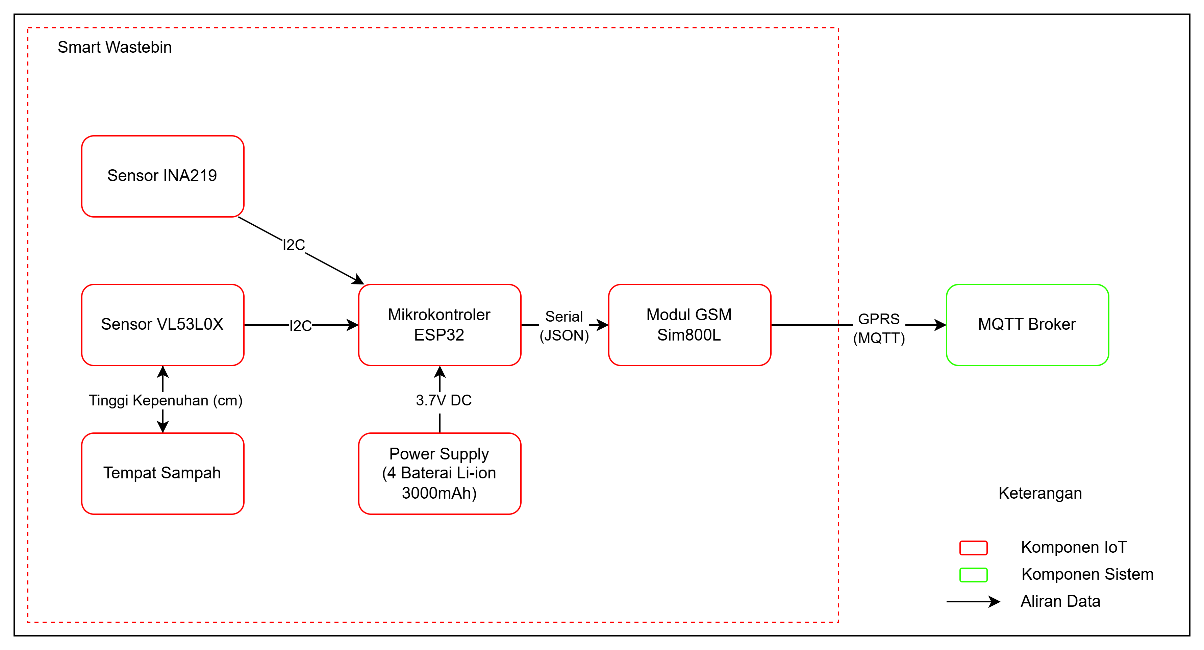
\includegraphics[width=0.85\textwidth]{images/blok-fungsional.png}
  % RENAME: image10.png → blok-fungsional.png
\end{figure}

Tabel \ref{tab:fungsi-komponen} menyajikan deskripsi fungsional setiap komponen perangkat.

\begin{table}[H]
  \caption{Fungsi Setiap Komponen \textit{Smart Waste Bin}}
  \label{tab:fungsi-komponen}
  \begin{tabularx}{\textwidth}{| l | X |}
    \hline
    \textbf{Komponen} & \textbf{Fungsi} \\
    \hline
    Sensor VL53L0X V2 & Mengukur jarak antara sensor dengan permukaan sampah \\
    \hline
    Sensor INA219 & Mengukur tegangan dan arus baterai untuk \textit{monitoring} daya \\
    \hline
    Mikrokontroler ESP32 & Memproses data sensor dan mengatur jadwal pengiriman \\
    \hline
    Modul GSM SIM800L & Mengirimkan data ke MQTT \textit{broker} melalui jaringan seluler \\
    \hline
    Baterai 18650 Li-Ion & Menyediakan sumber daya untuk seluruh komponen \\
    \hline
  \end{tabularx}
\end{table}

Mekanisme kerja perangkat secara fungsional adalah sebagai berikut. Setiap interval waktu tertentu, mikrokontroler terbangun dari mode \textit{deep sleep} dan mengaktifkan seluruh komponen. Sensor VL53L0X V2 melakukan pembacaan jarak, kemudian mikrokontroler mengambil nilai median untuk mengurangi \textit{noise}. Nilai jarak dikonversi menjadi persentase tingkat kepenuhan menggunakan Persamaan \ref{eq:fill-level}.

\begin{equation}
  \text{Fill Level} (\%) = \frac{\text{Kedalaman Bin} - \text{Jarak Terukur}}{\text{Kedalaman Bin}} \times 100
  \label{eq:fill-level}
\end{equation}
\eqcaption{Persamaan Konversi Tingkat Kepenuhan}

dengan kedalaman \textit{bin} sebesar 1000 mm. Persamaan ini memetakan seluruh rentang jarak terukur (0--1000 mm) menjadi nilai \textit{fillLevel} (0--100\%) secara linier dan kontinu, sehingga tidak terdapat rentang jarak yang tidak terdefinisi. Sebagai ilustrasi, Tabel \ref{tab:konversi-filllevel} menyajikan pemetaan beberapa rentang jarak terukur terhadap nilai \textit{fillLevel} yang dihasilkan.

\begin{table}[H]
  \caption{Pemetaan Jarak Terukur terhadap \textit{Fill Level}}
  \label{tab:konversi-filllevel}
  \centering
  \begin{tabular}{| c | c | c |}
    \hline
    \textbf{Jarak Terukur (mm)} & \textbf{\textit{Fill Level} (\%)} & \textbf{Interpretasi} \\
    \hline
    0--99 & 91--100 & Hampir penuh \\
    \hline
    100--299 & 71--90 & Terisi banyak \\
    \hline
    300--499 & 51--70 & Terisi sedang \\
    \hline
    500--699 & 31--50 & Terisi sebagian \\
    \hline
    700--899 & 11--30 & Hampir kosong \\
    \hline
    900--1000 & 0--10 & Kosong \\
    \hline
  \end{tabular}
\end{table}

Untuk menjaga validitas data, pembacaan jarak yang berada di luar rentang fisik \textit{bin} ditangani secara khusus. Jarak terukur yang melebihi 1000 mm (yang secara teoretis menghasilkan \textit{fillLevel} negatif) dibatasi (\textit{clamp}) menjadi 0\%, sedangkan pembacaan yang lebih kecil dari 0 mm dibatasi menjadi 100\%. Apabila sensor mengalami \textit{timeout} atau gagal melakukan pembacaan, nilai \textit{fillLevel} diisi dengan -1 sebagai penanda \textit{error}, yang kemudian disaring pada tahap praproses data. Dengan demikian, setiap kemungkinan nilai pembacaan, baik di dalam maupun di luar rentang valid, memiliki penanganan yang terdefinisi.

Sensor INA219 mengukur tegangan dan arus baterai untuk menghitung \textit{State of Charge} (SoC) menggunakan Persamaan \ref{eq:battery-percent}.

\begin{equation}
  \text{Battery Percent} (\%) = \frac{\text{Tegangan Terukur} - 5{,}60}{0{,}028}
  \label{eq:battery-percent}
\end{equation}
\eqcaption{Persamaan Perhitungan State of Charge Baterai}

Jika tegangan baterai di bawah 5,6V atau persentase di bawah 30\%, perangkat memasuki mode \textit{sleep forever} untuk mencegah kerusakan baterai akibat \textit{over-discharge}. Data yang telah diproses dikirimkan ke MQTT \textit{broker}, kemudian mikrokontroler kembali ke mode \textit{deep sleep}.

\subsection{Spesifikasi \textit{Interface} Data}

\textit{Interface} antara perangkat IoT dengan sistem internal didefinisikan melalui format data yang dikirimkan via protokol MQTT. Tabel \ref{tab:spesifikasi-mqtt} menyajikan spesifikasi koneksi MQTT yang digunakan.

\begin{table}[H]
  \caption{Spesifikasi Konektivitas MQTT}
  \label{tab:spesifikasi-mqtt}
  \begin{tabularx}{\textwidth}{| l | X |}
    \hline
    \textbf{Aspek} & \textbf{Nilai} \\
    \hline
    \textit{Broker} & Disediakan oleh vendor \\
    \hline
    \textit{Topic Pattern} & \texttt{wp2/basic\_01}; \texttt{wp2/basic\_02}; \texttt{wp2/basic\_03} \\
    \hline
    QoS \textit{Level} & 0 (default) \\
    \hline
    \textit{Authentication} & \textit{Username} dan \textit{password} (disediakan vendor) \\
    \hline
  \end{tabularx}
\end{table}

Data dikirimkan dalam format JSON. Tabel \ref{tab:payload-data} menyajikan spesifikasi setiap \textit{field} pada \textit{payload} data perangkat.

\begin{longtable}{| l | l | p{5.5cm} | l |}
  \caption{\textit{Payload} Data Perangkat}
  \label{tab:payload-data} \\
    \hline
    \textbf{\textit{Field}} & \textbf{Tipe Data} & \textbf{Deskripsi} & \textbf{Contoh} \\
    \hline
  \endfirsthead
    \hline
    \textbf{\textit{Field}} & \textbf{Tipe Data} & \textbf{Deskripsi} & \textbf{Contoh} \\
    \hline
  \endhead
    \hline
  \endfoot
    \texttt{sensor\_id} & String & Identifier unik perangkat & \texttt{"1"} \\
    \hline
    \texttt{tegangan} & Float & Tegangan baterai (Volt) & \texttt{7.25} \\
    \hline
    \texttt{arus} & Float & Arus perangkat (mA) & \texttt{100} \\
    \hline
    \texttt{daya} & Float & Daya terpakai (mW) & \texttt{727.4} \\
    \hline
    \texttt{battPercent} & Float & Persentase baterai (0--100) & \texttt{58.3} \\
    \hline
    \texttt{Ina219\_avail} & Boolean & Status ketersediaan sensor INA219 & \texttt{true} \\
    \hline
    \texttt{fillLevel} & Integer & Tingkat kepenuhan (0--100, atau -1 jika \textit{error}) & \texttt{65} \\
    \hline
    \texttt{dist} & Integer & Jarak terukur (mm, atau -1 jika \textit{error}) & \texttt{490} \\
    \hline
    \texttt{vol} & Integer & Volume sampah (dm³) & \texttt{38} \\
    \hline
    \texttt{sensor\_status} & String & Status sensor jarak & \texttt{"online"} \\
    \hline
    \texttt{vl53l0x\_avail} & Integer & Ketersediaan sensor (1=\textit{available}, 0=\textit{not}) & \texttt{1} \\
    \hline
    \texttt{event} & String & Tipe \textit{event} & \texttt{"DataUpdate"} \\
    \hline
\end{longtable}

Gambar \ref{fig:payload-contoh} menunjukkan contoh \textit{payload} data yang dikirimkan oleh perangkat.

\begin{figure}[H]
  \caption{Contoh \textit{Payload} Data Perangkat}
  \label{fig:payload-contoh}
  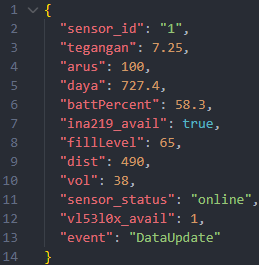
\includegraphics[width=0.45\textwidth]{images/payload-contoh.png}
  % RENAME: image11.png → payload-contoh.png
\end{figure}

% ============================================================
\section{Perancangan Adaptasi \textit{Firmware}}
\label{sec:perancangan-firmware}
% ============================================================

Sebagaimana diidentifikasi pada Subbab \ref{sec:analisis-kondisi}, perangkat \textit{Smart Waste Bin} yang tersedia memiliki konfigurasi \textit{firmware} yang dirancang untuk skala perkotaan. Untuk menyesuaikan dengan kebutuhan lingkungan kampus, dirancang lima adaptasi \textit{firmware}. Tabel \ref{tab:peningkatan-firmware} menyajikan ringkasan adaptasi yang dirancang.

\begin{table}[H]
  \caption{Rancangan Adaptasi \textit{Firmware}}
  \label{tab:peningkatan-firmware}
  \begin{tabularx}{\textwidth}{| X | X | X |}
    \hline
    \textbf{Aspek} & \textbf{Sebelum} & \textbf{Sesudah} \\
    \hline
    Interval Pengambilan Data & 8 jam & 2 jam 30 menit \\
    \hline
    Pembacaan Sensor & \textit{Single reading} & 5 \textit{readings} dengan \textit{median filter} \\
    \hline
    \textit{Error Handling} & Tidak ada mekanisme \textit{recovery} & \textit{Auto-recovery} dengan \textit{power cycle} \\
    \hline
    \textit{Warm-up} Sensor & Langsung pembacaan & 3x \textit{warm-up readings} sebelum pengukuran \\
    \hline
    Optimasi Daya & Standard GPIO & GPIO \textit{isolation} untuk mencegah \textit{floating} \\
    \hline
  \end{tabularx}
\end{table}

\subsection{Perancangan Perubahan Interval Pengambilan Data}

Interval pengambilan data pada kondisi awal adalah 8 jam, yang merupakan konfigurasi bawaan pada \textit{firmware} vendor (didefinisikan melalui konstanta \texttt{TIME\_TO\_SLEEP} pada kode sumber perangkat). Konfigurasi ini dirancang untuk konteks pemantauan kontainer sampah skala perkotaan yang volumenya besar dan laju pengisiannya lambat, sehingga pelaporan tiga kali sehari dinilai memadai oleh vendor sekaligus menghemat daya baterai.

Untuk konteks kampus, interval tersebut diubah menjadi 2 jam 30 menit berdasarkan pertimbangan berikut. Pertama, dari sisi kebutuhan resolusi data: dinamika pembuangan sampah kampus terkonsentrasi pada jam-jam tertentu dalam rentang jam aktif (sekitar 07:00--19:00), sehingga interval 8 jam yang hanya menghasilkan sekitar 3 titik data per hari berisiko melewatkan transisi antar sesi aktivitas (pagi, siang, sore). Interval 2,5 jam menghasilkan 8 sampai 9 titik data per hari, yang berarti terdapat sekitar 4--5 titik data dalam rentang jam aktif kampus, cukup untuk membedakan aktivitas antar sesi tanpa celah pengamatan yang lebar.

Kedua, dari sisi batasan daya: setiap siklus pengiriman mengaktifkan modul GSM SIM800L yang merupakan konsumen daya terbesar pada perangkat. Memperpendek interval lebih jauh (misalnya 1 jam, yang berarti 24 siklus per hari) akan melipatgandakan frekuensi aktivasi GSM hingga hampir tiga kali lipat dibandingkan interval 2,5 jam, sehingga secara proporsional memperpendek umur baterai dan meningkatkan frekuensi penggantian baterai di lapangan. Interval 2,5 jam dipilih sebagai titik keseimbangan: resolusi data memadai untuk analisis pola harian, sementara frekuensi aktivasi GSM (9--10 siklus per hari) masih berada pada tingkat yang memungkinkan perangkat beroperasi beberapa hari tanpa penggantian baterai. Dengan demikian, nilai 2,5 jam bukan angka arbitrer, melainkan hasil pertimbangan rekayasa antara kebutuhan resolusi analisis dan keterbatasan daya perangkat.

\subsection{Perancangan \textit{Median Filter}}

Pembacaan sensor VL53L0X ditingkatkan dari \textit{single reading} menjadi 5 kali pembacaan dengan pengambilan nilai median. Pendekatan ini dipilih karena median lebih \textit{robust} terhadap \textit{outlier} dibandingkan rata-rata (\textit{mean}). Mekanisme yang dirancang adalah sebagai berikut: sensor melakukan 5 kali pembacaan dengan interval 100ms, setiap pembacaan dicek validitasnya (\textit{timeout} dan \textit{range} 0--1400mm), nilai-nilai valid diurutkan, nilai median diambil sebagai hasil akhir, dan jika \textit{valid count} $<$ 3 digunakan rata-rata sebagai \textit{fallback}.

\subsection{Perancangan Mekanisme \textit{Auto-recovery}}

Sensor VL53L0X dapat mengalami kondisi \textit{hang} yang menyebabkan \textit{timeout} berulang. Kondisi \textit{trigger recovery} didefinisikan sebagai \textit{timeout} yang terjadi $\geq$ 3 kali dari 5 pembacaan, atau tidak ada pembacaan valid sama sekali. Langkah \textit{recovery} yang dirancang adalah: (1) \textit{stop continuous mode} pada sensor, (2) \textit{soft reset} dengan re-inisialisasi sensor, (3) jika \textit{soft reset} gagal, lakukan \textit{power cycle} (matikan daya sensor 500ms lalu hidupkan kembali), (4) re-inisialisasi I2C dan sensor, dan (5) jika masih gagal, tandai sensor sebagai \textit{offline}.

\subsection{Perancangan \textit{Warm-up} Sensor}

Sensor VL53L0X memerlukan beberapa pembacaan awal sebelum menghasilkan nilai yang stabil, karena pembacaan pertama setelah inisialisasi cenderung tidak representatif. Mekanisme \textit{warm-up} yang dirancang adalah: sensor diinisialisasi dan dikonfigurasi dengan \textit{timing budget} 200ms, mode \textit{continuous measurement} diaktifkan dengan interval 200ms, kemudian tiga pembacaan \textit{dummy} dilakukan dengan jeda 200ms per pembacaan tanpa menggunakan nilainya. Setelah \textit{warm-up} selesai, sensor dinyatakan siap untuk pengukuran aktual.

\subsection{Perancangan Optimasi Daya}

Dua mekanisme optimasi daya dirancang untuk memperpanjang masa operasi baterai. Pertama, \textit{GPIO Isolation}: sebelum \textit{deep sleep}, seluruh GPIO yang digunakan di-\textit{hold} pada kondisi LOW untuk mencegah \textit{floating state} yang dapat menyebabkan konsumsi daya tidak perlu. Kedua, \textit{proper shutdown sequence}: urutan mematikan komponen dioptimalkan untuk memastikan tidak ada komponen yang tertinggal dalam kondisi aktif. Tabel \ref{tab:urutan-shutdown} menyajikan urutan \textit{shutdown} yang dirancang.

\begin{table}[H]
  \caption{Urutan \textit{Shutdown} Perangkat}
  \label{tab:urutan-shutdown}
  \begin{tabularx}{\textwidth}{| l | l | X |}
    \hline
    \textbf{Step} & \textbf{Aksi} & \textbf{Keterangan} \\
    \hline
    1 & \textit{Stop} sensor \textit{continuous} & Menghentikan mode pembacaan kontinyu VL53L0X \\
    \hline
    2 & \textit{Disconnect} MQTT & Menutup koneksi MQTT dengan \textit{broker} \\
    \hline
    3 & GPRS \textit{disconnect} & Memutus koneksi data seluler \\
    \hline
    4 & Modem \textit{power off} & Mematikan modem SIM800L \\
    \hline
    5 & GPIO LOW & Set semua GPIO ke LOW (TRIG, TRIG\_SENSOR, LED) \\
    \hline
    6 & GPIO \textit{hold enable} & Isolasi GPIO untuk mencegah \textit{floating} saat \textit{sleep} \\
    \hline
    7 & I2C \textit{end} & Menonaktifkan bus I2C \\
    \hline
    8 & Serial \textit{flush} \& \textit{end} & \textit{Flush buffer} serial dan nonaktifkan \\
    \hline
    9 & \textit{Deep sleep} & Masuk mode \textit{deep sleep} selama 2,5 jam \\
    \hline
  \end{tabularx}
\end{table}

% ============================================================
\section{Perancangan \textit{Middleware}}
\label{sec:perancangan-middleware}
% ============================================================

\textit{Middleware} merupakan komponen internal yang berfungsi sebagai jembatan antara perangkat IoT pada \textit{Network Layer} dengan komponen penyimpanan pada \textit{Application Layer}. Pada sistem ini, \textit{middleware} dirancang menggunakan Node-RED. Subbab ini berfokus pada \emph{rancangan} arsitektur \textit{flow} serta \emph{spesifikasi target} konfigurasi \textit{node} yang menjadi acuan, sedangkan realisasi konfigurasi aktual beserta pengujiannya dibahas pada Bab \ref{chap:implementasi}.

\subsection{Arsitektur \textit{Flow} Node-RED}

\textit{Flow} Node-RED untuk sistem pemantauan sampah berbasis \textit{Internet of Things} dirancang untuk menerima data dari tiga perangkat sensor secara paralel dan meneruskannya ke \textit{database}. Gambar \ref{fig:flow-nodered} menunjukkan rancangan alur pemrosesan data secara konseptual, mulai dari penerimaan pesan hingga penyimpanan ke \textit{database}.

\begin{figure}[H]
  \caption{Rancangan Alur Pemrosesan Data \textit{Middleware}}
  \label{fig:flow-nodered}
  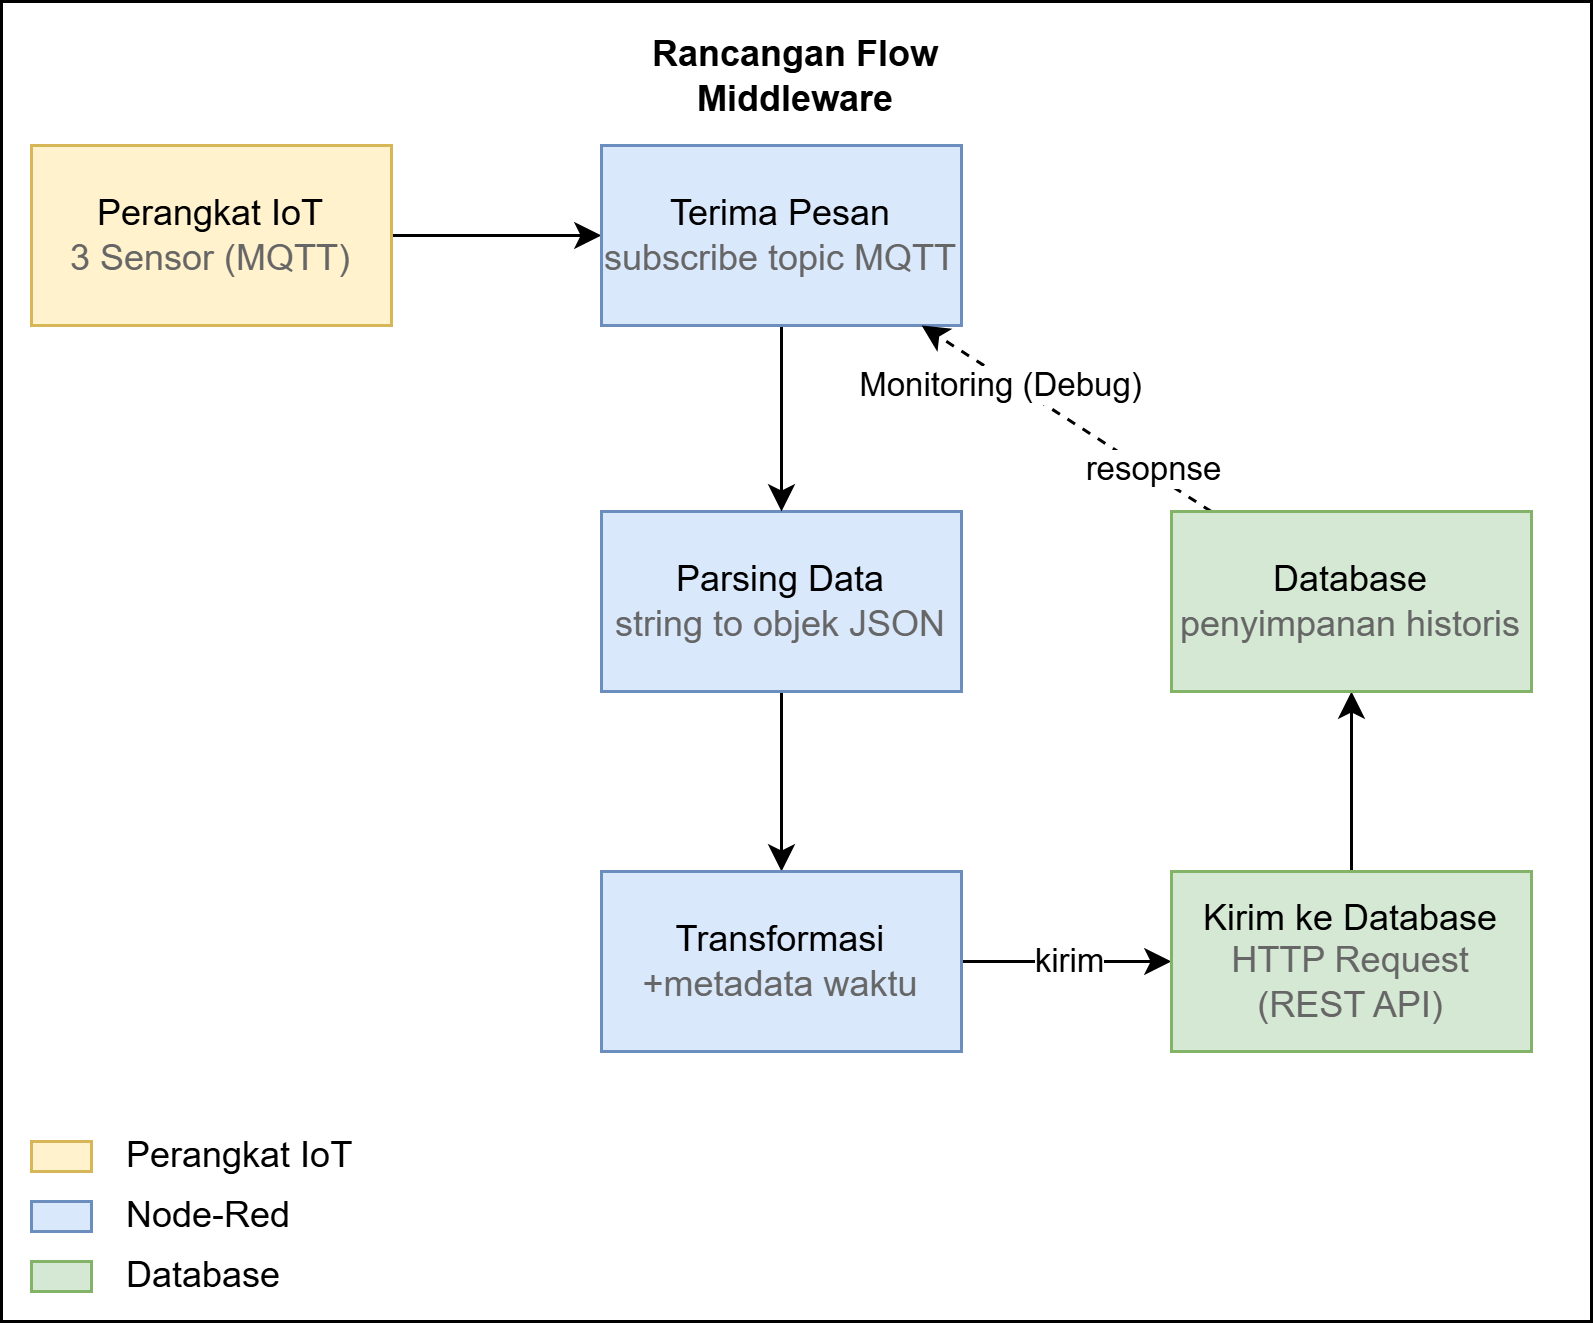
\includegraphics[width=\textwidth]{images/rancangan-flow-middleware.png}
  % CATATAN: gunakan diagram alur generik (mis. dibuat di draw.io),
  %          BUKAN tangkapan layar flow Node-RED yang sudah jadi.
  %          Tangkapan layar implementasi aktual ditempatkan di Bab V.
\end{figure}

Berdasarkan Gambar \ref{fig:flow-nodered}, \textit{middleware} dirancang menggunakan beberapa kelompok \textit{node} dengan peran yang berbeda. Tabel \ref{tab:tipe-node} menyajikan ringkasan tipe \textit{node} yang direncanakan beserta fungsinya.

\begin{table}[H]
  \caption{Tipe \textit{Node} pada \textit{Flow} Node-RED}
  \label{tab:tipe-node}
  \begin{tabularx}{\textwidth}{| l | l | X |}
    \hline
    \textbf{Tipe \textit{Node}} & \textbf{Jumlah} & \textbf{Fungsi} \\
    \hline
    Inject & 7 & Simulasi data untuk pengujian \\
    \hline
    MQTT In & 3 & Menerima data dari MQTT \textit{broker} \\
    \hline
    JSON & 3 & \textit{Parsing} string JSON ke objek \\
    \hline
    Function & 3 & Transformasi dan penambahan metadata \\
    \hline
    HTTP Request & 3 & Pengiriman data ke \textit{database} \\
    \hline
    Debug & 6 & \textit{Monitoring} data dan \textit{response} \\
    \hline
  \end{tabularx}
\end{table}

\subsection{Rancangan Alur Pemrosesan Data}

Alur pemrosesan data pada \textit{middleware} dirancang sebagai berikut. Pertama, pesan dari \textit{broker} MQTT diterima oleh \textit{node} penerima. Kedua, \textit{payload} dalam format string dikonversi menjadi objek terstruktur. Ketiga, dilakukan transformasi \textit{field} dan penambahan metadata berupa \textit{timestamp} server. Keempat, data yang telah diolah dikirimkan ke \textit{database} melalui REST API. \textit{Response} dari \textit{database} dipantau untuk memastikan keberhasilan penyimpanan. Spesifikasi konfigurasi aktual setiap \textit{node} beserta nilai parameternya dibahas pada Subbab \ref{sec:impl-middleware}.

\subsection{Spesifikasi \textit{Deployment} \textit{Middleware}}

Tabel \ref{tab:deployment-nodered} menyajikan spesifikasi \textit{deployment} dan operasional \textit{middleware} Node-RED yang direncanakan untuk sistem.

\begin{table}[H]
  \caption{Spesifikasi \textit{Deployment} dan Operasional Node-RED}
  \label{tab:deployment-nodered}
  \begin{tabularx}{\textwidth}{| l | X |}
    \hline
    \textbf{Aspek} & \textbf{Spesifikasi} \\
    \hline
    \textit{Platform} & Node-RED v4.1.3 \\
    \hline
    \textit{Runtime} & Node.js v24.12.0 \\
    \hline
    \textit{Hosting} & \textit{Server} lokal menggunakan komputer peneliti yang dinyalakan selama penelitian \\
    \hline
    \textit{Auto-connect} & \textit{Enabled} (reconnect otomatis ke MQTT \textit{broker}) \\
    \hline
    \textit{Flow} Name & MQTT to Supabase \textit{Flow} \\
    \hline
  \end{tabularx}
\end{table}

% ============================================================
\section{Perancangan \textit{Database}}
\label{sec:perancangan-database}
% ============================================================

\textit{Database} merupakan komponen pada \textit{Application Layer} yang berfungsi untuk menyimpan seluruh data pembacaan sensor secara persisten dan terstruktur. Sistem ini menggunakan Supabase yang merupakan \textit{platform Backend-as-a-Service} berbasis PostgreSQL.

\subsection{Spesifikasi \textit{Platform Database}}

Supabase dipilih karena menyediakan beberapa keunggulan: berbasis PostgreSQL sebagai \textit{database} relasional \textit{open source} dengan fitur lengkap, REST API \textit{built-in} yang memungkinkan akses data tanpa perlu mengembangkan \textit{backend} terpisah, dan \textit{dashboard} web untuk manajemen \textit{database}. Tabel \ref{tab:spesifikasi-database} menyajikan spesifikasi \textit{platform database}.

\begin{table}[H]
  \caption{Spesifikasi \textit{Platform Database}}
  \label{tab:spesifikasi-database}
  \begin{tabularx}{\textwidth}{| p{4cm} | X |}
    \hline
    \textbf{Aspek} & \textbf{Spesifikasi} \\
    \hline
    \textit{Platform} & Supabase \\
    \hline
    \textit{Database Engine} & PostgreSQL \\
    \hline
    \textit{Hosting} & Supabase \textit{Cloud} (Free Tier) \\
    \hline
    Akses Data & REST API (PostgREST) \\
    \hline
    Autentikasi API & API Key (anon key) \\
    \hline
    \textit{Dashboard} & \textit{Web-based} \\
    \hline
  \end{tabularx}
\end{table}

\subsection{Desain Skema \textit{Database}}

Sistem menggunakan satu tabel utama bernama \texttt{sensor\_data} untuk menyimpan seluruh data pembacaan sensor. Desain ini dipilih karena data yang dikumpulkan bersifat \textit{time-series} dengan struktur yang seragam dari semua perangkat. Gambar \ref{fig:tabel-sensordata} menunjukkan struktur tabel \texttt{sensor\_data}.

\begin{figure}[H]
  \caption{Struktur Tabel \texttt{sensor\_data} pada Supabase}
  \label{fig:tabel-sensordata}
  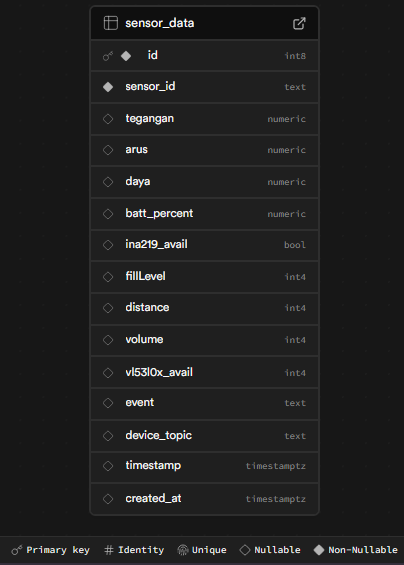
\includegraphics[width=0.5\textwidth]{images/tabel-sensordata.png}
  % RENAME: image13.png → tabel-sensordata.png
\end{figure}

Tabel \ref{tab:detail-sensordata} menyajikan spesifikasi setiap kolom pada tabel \texttt{sensor\_data}.

\begin{longtable}{| p{2.6cm} | p{1.8cm} | p{2.6cm} | p{5cm} |}
  \caption{Detail Kolom Tabel \texttt{sensor\_data}}
  \label{tab:detail-sensordata} \\
    \hline
    \textbf{Kolom} & \textbf{Tipe Data} & \textbf{\textit{Constraint}} & \textbf{Deskripsi} \\
    \hline
  \endfirsthead
    \hline
    \textbf{Kolom} & \textbf{Tipe Data} & \textbf{\textit{Constraint}} & \textbf{Deskripsi} \\
    \hline
  \endhead
    \hline
  \endfoot
    \texttt{id} & int8 & PK, Auto-increment & Identifier unik record \\
    \hline
    \texttt{sensor\_id} & text & Not Null & Identifier perangkat sensor \\
    \hline
    \texttt{tegangan} & Numeric & Nullable & Tegangan baterai (Volt) \\
    \hline
    \texttt{arus} & Numeric & Nullable & Arus baterai (mA) \\
    \hline
    \texttt{daya} & Numeric & Nullable & Daya terpakai (mW) \\
    \hline
    \texttt{batt\_percent} & Numeric & Nullable & Persentase baterai (\%) \\
    \hline
    \texttt{ina219\_avail} & Bool & Nullable & Status ketersediaan sensor INA219 \\
    \hline
    \texttt{fillLevel} & Int4 & Nullable & Tingkat kepenuhan (0--100\%) \\
    \hline
    \texttt{distance} & Int4 & Nullable & Jarak terukur (mm) \\
    \hline
    \texttt{volume} & Int4 & Nullable & Volume sampah (dm³) \\
    \hline
    \texttt{vl53l0x\_avail} & Int4 & Nullable & Ketersediaan sensor VL53L0X (1/0) \\
    \hline
    \texttt{event} & text & Nullable & Tipe \textit{event} (DataUpdate, LowBattery, dll.) \\
    \hline
    \texttt{device\_topic} & text & Nullable & \textit{Topic} MQTT sumber data \\
    \hline
    \texttt{timestamp} & timestamptz & Nullable & Waktu pembacaan sensor (dari perangkat) \\
    \hline
    \texttt{created\_at} & timestamptz & Nullable & Waktu data disimpan di \textit{database} \\
    \hline
\end{longtable}

\textit{Field} \texttt{timestamp} mencatat waktu pembacaan di perangkat IoT, sedangkan \texttt{created\_at} mencatat waktu data diterima dan disimpan di \textit{database}. Selisih antara kedua \textit{timestamp} tersebut menunjukkan latensi transmisi data dari perangkat ke \textit{database}.

% ============================================================
\section{Perancangan \textit{Dashboard}}
\label{sec:perancangan-dashboard}
% ============================================================

\textit{Dashboard} merupakan komponen pada \textit{Application Layer} yang berfungsi sebagai antarmuka pengguna untuk memvisualisasikan data sensor. Sistem ini menggunakan Next.js sebagai \textit{framework} utama.

\subsection{Arsitektur \textit{Dashboard}}

\textit{Dashboard} dibangun menggunakan arsitektur \textit{client-server} dengan Next.js. Komponen \textit{frontend} mengambil data dari \textit{backend} melalui API Routes yang terhubung ke \textit{database} Supabase menggunakan Drizzle ORM. Tabel \ref{tab:teknologi-dashboard} menyajikan komponen teknologi yang digunakan.

\begin{table}[H]
  \caption{Komponen Teknologi \textit{Dashboard}}
  \label{tab:teknologi-dashboard}
  \begin{tabularx}{\textwidth}{| l | l | X |}
    \hline
    \textbf{Komponen} & \textbf{Teknologi} & \textbf{Fungsi} \\
    \hline
    Framework & Next.js & \textit{Server-side rendering} dan routing \\
    \hline
    UI \textit{Library} & React & Komponen antarmuka pengguna \\
    \hline
    Styling & Tailwind CSS & CSS framework \\
    \hline
    \textit{Charting} & Recharts & \textit{Library} visualisasi data \\
    \hline
    ORM & Drizzle ORM & \textit{Object-Relational Mapping} untuk akses \textit{database} \\
    \hline
    \textit{Database} & Supabase PostgreSQL & Penyimpanan data \\
    \hline
  \end{tabularx}
\end{table}

\subsection{Perancangan API}

\textit{Dashboard} berkomunikasi dengan \textit{database} melalui API Routes pada endpoint \texttt{/api/sensor-data}. Tabel \ref{tab:spesifikasi-api} menyajikan spesifikasi API \textit{endpoint} yang dirancang.

\begin{table}[H]
  \caption{Spesifikasi API \textit{Endpoint}}
  \label{tab:spesifikasi-api}
  \begin{tabularx}{\textwidth}{| l | l | X |}
    \hline
    \textbf{Metode} & \textbf{Parameter} & \textbf{Fungsi} \\
    \hline
    GET & \texttt{sensorId}, \texttt{timerange}, \texttt{limit} & Mengambil data sensor dengan \textit{filter} \\
    \hline
    POST & Body: sensor data object & Menyimpan data sensor baru \\
    \hline
    PUT & Body: id, update \textit{fields} & Memperbarui data sensor \\
    \hline
    DELETE & \texttt{id}, \texttt{sensorId}, \texttt{olderThan} & Menghapus data sensor \\
    \hline
  \end{tabularx}
\end{table}

API GET mendukung parameter \texttt{timerange} dengan nilai sebagaimana pada Tabel \ref{tab:parameter-timerange}.

\begin{table}[H]
  \caption{Nilai Parameter \texttt{timerange}}
  \label{tab:parameter-timerange}
  \begin{tabularx}{\textwidth}{| l | X |}
    \hline
    \textbf{Nilai} & \textbf{Rentang Waktu} \\
    \hline
    \texttt{1h} & 1 jam terakhir \\
    \hline
    \texttt{24h} & 24 jam terakhir (\textit{default}) \\
    \hline
    \texttt{7d} & 7 hari terakhir \\
    \hline
    \texttt{30d} & 30 hari terakhir \\
    \hline
  \end{tabularx}
\end{table}

\subsection{Perancangan Antarmuka}

Antarmuka \textit{dashboard} dirancang terdiri dari enam komponen utama:

\begin{enumerate}
  \item \textbf{\textit{Header Section}}: menampilkan judul aplikasi, tombol \textit{refresh} manual, dan informasi \textit{timestamp} pembaruan terakhir.
  \item \textbf{\textit{Sensor Status Cards}}: kartu status untuk setiap sensor aktif, menampilkan \textit{fill level} dengan \textit{progress bar} berwarna (hijau $\leq$70\%, kuning 71--85\%, merah $>$85\%), persentase baterai, konsumsi daya, \textit{topic} MQTT, dan \textit{timestamp} terakhir.
  \item \textbf{\textit{Control Panel}}: \textit{dropdown} pemilihan sensor dan rentang waktu, serta informasi jumlah \textit{data points} dan \textit{active sensors}.
  \item \textbf{Visualisasi Data}: dua \textit{chart} interaktif, yaitu \textit{line chart} tren tingkat kepenuhan dan \textit{dual-axis line chart} baterai dan konsumsi daya.
  \item \textbf{\textit{Recent Sensor Readings}}: tabel 10 pembacaan terbaru dengan \textit{progress bar} mini dan \textit{status indicator}.
  \item \textbf{\textit{System Analytics}}: lima metrik agregat sistem (Total Records, Active Sensors, Avg Battery, Avg Power, Critical Alerts).
\end{enumerate}

\textit{Dashboard} dirancang dengan \textit{auto-refresh} setiap 30 detik menggunakan \texttt{useEffect} Hook dengan \textit{cleanup function} untuk mencegah \textit{memory leak}.

\subsection{Spesifikasi \textit{Hosting Dashboard}}

Tabel \ref{tab:hosting-dashboard} menyajikan spesifikasi \textit{hosting} \textit{dashboard} pada \textit{platform} Vercel.

\begin{table}[H]
  \caption{Spesifikasi \textit{Hosting Dashboard}}
  \label{tab:hosting-dashboard}
  \begin{tabularx}{\textwidth}{| l | X |}
    \hline
    \textbf{Aspek} & \textbf{Spesifikasi} \\
    \hline
    \textit{Platform} & Vercel (\textit{free tier}) \\
    \hline
    \textit{Framework Preset} & Next.js \\
    \hline
    \textit{Build Command} & \texttt{next build} \\
    \hline
    \textit{Output Directory} & \texttt{.next} \\
    \hline
    \textit{Deployment Method} & Git Integration (\textit{Continuous Deployment}) \\
    \hline
    Domain & Subdomain Vercel (\texttt{*.vercel.app}) \\
    \hline
  \end{tabularx}
\end{table}

\textit{Deployment} dilakukan secara otomatis melalui integrasi dengan repositori Git. Setiap \textit{push} ke \textit{branch} utama akan memicu proses \textit{build} dan \textit{deployment} secara otomatis (\textit{Continuous Deployment}).
% ==========================================
% BAB V IMPLEMENTASI
% ==========================================
\cleardoublepage
\chapter{IMPLEMENTASI SISTEM \textit{SMART WASTE BIN}}
\label{chap:implementasi}

Bab ini merupakan bagian kedua dari realisasi tahap \textit{Prototype} dalam metodologi \textit{Design Thinking}. Berdasarkan rancangan pada Bab IV, bab ini menjelaskan implementasi aktual setiap komponen sistem \textit{Smart Waste Bin}, mencakup peningkatan \textit{firmware} perangkat IoT, konfigurasi \textit{middleware} Node-RED, pembuatan \textit{database} Supabase, dan pengembangan \textit{dashboard} Next.js. Setiap subbab menjelaskan teknologi dan \textit{tools} yang digunakan, langkah-langkah implementasi, serta hasil yang diperoleh.

% ============================================================
\section{Implementasi Peningkatan \textit{Firmware}}
\label{sec:impl-firmware}
% ============================================================

Implementasi peningkatan \textit{firmware} dilakukan pada perangkat \textit{Smart Waste Bin} menggunakan Arduino IDE dengan \textit{board package} ESP32. Lima peningkatan yang dirancang pada Subbab \ref{sec:perancangan-firmware} diimplementasikan secara bertahap dan diuji sebelum di-\textit{deploy} ke perangkat di lapangan.

\subsection{Implementasi Perubahan Interval Pengambilan Data}

Interval \textit{deep sleep} diubah dari 8 jam menjadi 2 jam 30 menit dengan mendefinisikan konstanta waktu tidur dalam satuan mikrodetik, sebagaimana ditunjukkan pada \textit{Listing} \ref{lst:interval}.

\begin{lstlisting}[caption={Implementasi Perubahan Interval Pengambilan Data}, label={lst:interval}, language=C++]
// ===== SLEEP CONFIG =====
// 2.5 jam = 150 menit
uint64_t TIME_TO_SLEEP = 150ULL * 60ULL * 1000000ULL;
\end{lstlisting}

Perubahan interval ini menghasilkan 8--9 titik data per hari per perangkat, meningkat signifikan dari sebelumnya yang hanya 3 titik data per hari dengan interval 8 jam.

\subsection{Implementasi \textit{Median Filter}}

Pembacaan sensor diubah dari \textit{single reading} menjadi 5 kali pembacaan dengan pengambilan nilai median menggunakan algoritma \textit{bubble sort}, sebagaimana ditunjukkan pada \textit{Listing} \ref{lst:median}.

\begin{lstlisting}[caption={Implementasi \textit{Median Filter} pada Pembacaan Sensor}, label={lst:median}, language=C++]
const int numReadings = 5;
int readings[numReadings];
int validCount = 0;

for (int i = 0; i < numReadings; i++) {
    int reading = sensor.readRangeContinuousMillimeters();
    if (!sensor.timeoutOccurred() && reading > 0 && reading <= 1400) {
        readings[validCount] = reading;
        validCount++;
    }
    delay(100);
}

// Bubble sort for median
for (int i = 0; i < validCount - 1; i++) {
    for (int j = i + 1; j < validCount; j++) {
        if (readings[i] > readings[j]) {
            int temp = readings[i];
            readings[i] = readings[j];
            readings[j] = temp;
        }
    }
}

if (validCount >= 3) {
    a = readings[validCount / 2]; // Get median
} else if (validCount > 0) {
    int sum = 0;
    for (int i = 0; i < validCount; i++) sum += readings[i];
    a = sum / validCount;  // Fallback: mean
}
\end{lstlisting}

Implementasi ini mengurangi \textit{noise} pada data sensor. Nilai median dari 5 pembacaan mencegah pembacaan \textit{outlier} tunggal mempengaruhi hasil akhir, khususnya mencegah lompatan 10\% pada \textit{fillLevel} akibat \textit{truncation integer} dari perbedaan 1 unit \textit{raw}.

\subsection{Implementasi Mekanisme \textit{Auto-recovery}}

Mekanisme \textit{auto-recovery} diimplementasikan untuk menangani kondisi \textit{hang} pada sensor VL53L0X, sebagaimana ditunjukkan pada \textit{Listing} \ref{lst:recovery} dan \textit{Listing} \ref{lst:powercycle}.

\begin{lstlisting}[caption={Implementasi \textit{Auto-recovery} Sensor}, label={lst:recovery}, language=C++]
// Auto-recovery if sensor hangs (>= 3 timeout dari 5 pembacaan)
if (timeoutCount >= 3 || validCount == 0) {
    sensor.stopContinuous();
    delay(100);

    // Try soft reset first
    if (sensor.init(true)) {
        sensor.setMeasurementTimingBudget(200000);
        sensor.startContinuous(200);
        return; // Soft reset OK
    }

    // Soft reset failed, power cycle
    powerCycleSensor();
    if (!sensor.init(true)) {
        readSensor = false; // Sensor offline
    }
}
\end{lstlisting}

\begin{lstlisting}[caption={Implementasi \textit{Power Cycle} Sensor}, label={lst:powercycle}, language=C++]
void powerCycleSensor() {
    digitalWrite(TRIG_SENSOR, LOW);  // Turn off sensor power
    delay(500);                       // Wait for capacitor discharge
    digitalWrite(TRIG_SENSOR, HIGH); // Turn on again
    delay(300);                       // Wait for sensor boot
    Wire.end();
    delay(50);
    Wire.begin();                     // Re-init I2C
}
\end{lstlisting}

Mekanisme ini berhasil mencegah \textit{data loss} akibat sensor \textit{hang} yang sebelumnya memerlukan \textit{reset} manual.

\subsection{Implementasi \textit{Warm-up} Sensor}

Mekanisme \textit{warm-up} diimplementasikan sebagai bagian dari fungsi \texttt{initVL53L0X()} dengan 3 pembacaan \textit{dummy} setelah inisialisasi, sebagaimana ditunjukkan pada \textit{Listing} \ref{lst:warmup}.

\begin{lstlisting}[caption={Implementasi \textit{Warm-up} Sensor}, label={lst:warmup}, language=C++]
sensor.setMeasurementTimingBudget(200000);
delay(100);
sensor.startContinuous(200);

// Warm-up readings --- nilai dibuang, hanya untuk stabilisasi
SerialMon.println(F("Warming up sensor..."));
for (int i = 0; i < 3; i++) {
    sensor.readRangeContinuousMillimeters();
    delay(200);
}
SerialMon.println(F("Sensor ready!"));
\end{lstlisting}

Pendekatan ini memastikan pembacaan pertama data aktual sudah dalam kondisi sensor yang stabil, mengurangi risiko nilai anomali di awal setiap siklus pengukuran.

\subsection{Implementasi Optimasi Daya}

Optimasi daya diimplementasikan melalui \textit{GPIO isolation} sebelum \textit{deep sleep} untuk mencegah \textit{floating state}, sebagaimana ditunjukkan pada \textit{Listing} \ref{lst:gpio}.

\begin{lstlisting}[caption={Implementasi \textit{GPIO Isolation}}, label={lst:gpio}, language=C++]
// Turn off all GPIO
digitalWrite(TRIG, LOW);
digitalWrite(TRIG_SENSOR, LOW);
digitalWrite(LED_READ, LOW);
digitalWrite(LED_NET, LOW);

// Isolate GPIO (prevent floating during sleep)
gpio_hold_en(GPIO_NUM_13); // TRIG (modem power)
gpio_hold_en(GPIO_NUM_23); // TRIG_SENSOR
gpio_hold_en(GPIO_NUM_18); // LED_NET
gpio_hold_en(GPIO_NUM_19); // LED_READ
gpio_deep_sleep_hold_en();
\end{lstlisting}

% ============================================================
\section{Implementasi \textit{Middleware}}
\label{sec:impl-middleware}
% ============================================================

Berdasarkan rancangan \textit{flow} dan spesifikasi \textit{node} pada Subbab \ref{sec:perancangan-middleware}, \textit{middleware} diimplementasikan menggunakan Node-RED v4.1.3 yang berjalan pada \textit{server} lokal dengan Node.js v24.12.0. Berbeda dengan Bab \ref{chap:perancangan} yang membahas rancangan, subbab ini menyajikan realisasi konfigurasi aktual setiap \textit{node} beserta pengujian alur data menggunakan \textit{node} Inject.

Gambar \ref{fig:flow-nodered-impl} menunjukkan realisasi \textit{flow} Node-RED yang telah dibangun, mencakup \textit{node} MQTT In, JSON, HTTP Request, Debug, dan Inject untuk ketiga sensor.

\begin{figure}[H]
  \caption{Realisasi \textit{Flow} Node-RED pada Node-RED Editor}
  \label{fig:flow-nodered-impl}
  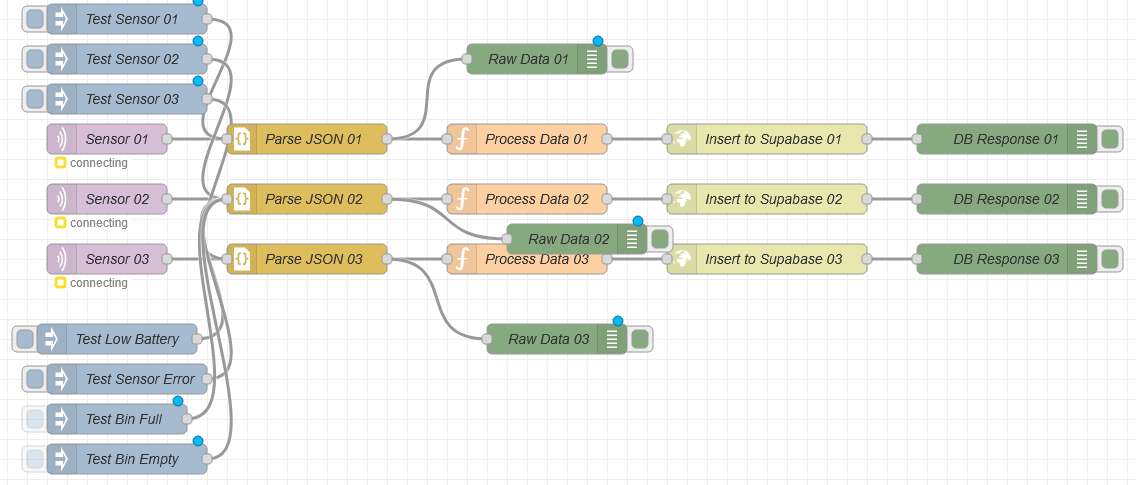
\includegraphics[width=\textwidth]{images/flow-nodered-impl.png}
  % RENAME: tangkapan layar (screenshot) flow Node-RED aktual dari Node-RED editor.
  %         Berbeda dengan Gambar di Bab IV yang berupa diagram alur generik (rancangan),
  %         gambar ini adalah realisasi nyata flow yang sudah dibangun.
\end{figure}

\subsection{Konfigurasi \textit{Node} MQTT In}

\textit{Node} MQTT In berfungsi sebagai \textit{subscriber} yang menerima data dari \textit{broker}. Tabel \ref{tab:konfigurasi-mqtt-node} menyajikan konfigurasi aktual yang digunakan.

\begin{table}[H]
  \caption{Konfigurasi \textit{Node} MQTT In}
  \label{tab:konfigurasi-mqtt-node}
  \begin{tabularx}{\textwidth}{| l | l | X |}
    \hline
    \textbf{Parameter} & \textbf{Nilai} & \textbf{Keterangan} \\
    \hline
    \textit{Server} & (IP \textit{Broker}) & Alamat MQTT \textit{broker} \\
    \hline
    Port & 1883 & Port default MQTT \\
    \hline
    \textit{Topic} & \texttt{wp2/basic\_01}, \texttt{wp2/basic\_02}, \texttt{wp2/basic\_03} & Satu \textit{topic} per sensor \\
    \hline
    \textit{Output} & Auto-detect & Otomatis deteksi tipe data \\
    \hline
  \end{tabularx}
\end{table}

\subsection{Konfigurasi \textit{Node} JSON}

\textit{Node} JSON mengkonversi \textit{payload} dari format string JSON menjadi objek JavaScript yang dapat diproses lebih lanjut. Tabel \ref{tab:impl-konfigurasi-json} menyajikan konfigurasi yang digunakan.

\begin{table}[H]
  \caption{Konfigurasi \textit{Node} JSON}
  \label{tab:impl-konfigurasi-json}
  \begin{tabularx}{\textwidth}{| l | l | X |}
    \hline
    \textbf{Parameter} & \textbf{Nilai} & \textbf{Keterangan} \\
    \hline
    Action & Convert between JSON String \& Object & Mengubah string ke objek \\
    \hline
    Property & msg.payload & Lokasi data yang dikonversi \\
    \hline
    Format JSON String & Tidak dicentang & \textit{Output} berupa objek, bukan string \\
    \hline
  \end{tabularx}
\end{table}

\subsection{Konfigurasi \textit{Node} HTTP Request}

\textit{Node} HTTP Request mengirimkan data ke \textit{database} Supabase menggunakan REST API. Tabel \ref{tab:konfigurasi-http} menyajikan parameter konfigurasinya, dan Tabel \ref{tab:konfigurasi-headers} menyajikan \textit{header} autentikasi yang digunakan.

\begin{table}[H]
  \caption{Konfigurasi \textit{Node} HTTP Request}
  \label{tab:konfigurasi-http}
  \begin{tabularx}{\textwidth}{| l | X |}
    \hline
    \textbf{Parameter} & \textbf{Nilai} \\
    \hline
    Method & POST \\
    \hline
    URL & \texttt{https://[project-ref]\allowbreak.supabase.co\allowbreak/rest\allowbreak/v1\allowbreak/sensor\_data} \\
    \hline
    \textit{Payload} & Dikirim sebagai \textit{request body} \\
    \hline
    Return & UTF-8 String \\
    \hline
  \end{tabularx}
\end{table}

\begin{table}[H]
  \caption{Konfigurasi HTTP \textit{Headers}}
  \label{tab:konfigurasi-headers}
  \begin{tabularx}{\textwidth}{| l | l | X |}
    \hline
    \textbf{\textit{Header}} & \textbf{Nilai} & \textbf{Keterangan} \\
    \hline
    \texttt{apikey} & [Supabase anon key] & API key untuk autentikasi \\
    \hline
    \texttt{Authorization} & Bearer [anon key] & Token autentikasi \\
    \hline
    \texttt{Content-Type} & application/json & Format data yang dikirim \\
    \hline
    \texttt{Prefer} & return=representation & Mengembalikan data yang berhasil disimpan \\
    \hline
  \end{tabularx}
\end{table}

\subsection{Konfigurasi \textit{Node} Debug}

\textit{Node} Debug menampilkan data pada \textit{sidebar} Node-RED untuk keperluan \textit{monitoring} dan \textit{debugging}. Tabel \ref{tab:impl-konfigurasi-debug} menyajikan konfigurasi yang digunakan.

\begin{table}[H]
  \caption{Konfigurasi \textit{Node} Debug}
  \label{tab:impl-konfigurasi-debug}
  \begin{tabularx}{\textwidth}{| l | l | X |}
    \hline
    \textbf{Nama \textit{Node}} & \textbf{\textit{Output}} & \textbf{Fungsi} \\
    \hline
    \textit{Raw data} 01/02/03 & msg.payload & Menampilkan data mentah setelah \textit{parsing} JSON \\
    \hline
    Authorization & msg.payload & Menampilkan \textit{response} dari Supabase \\
    \hline
  \end{tabularx}
\end{table}

\subsection{Konfigurasi \textit{Node} Inject}

\textit{Node} Inject digunakan untuk pengujian \textit{flow} tanpa menunggu data dari perangkat IoT. Tabel \ref{tab:impl-konfigurasi-inject} menyajikan daftar skenario pengujian yang diimplementasikan.

\begin{table}[H]
  \caption{Konfigurasi \textit{Node} Inject untuk Pengujian}
  \label{tab:impl-konfigurasi-inject}
  \begin{tabularx}{\textwidth}{| l | X | X |}
    \hline
    \textbf{Nama \textit{Node}} & \textbf{Skenario} & \textbf{Karakteristik Data} \\
    \hline
    Test Sensor 01/02/03 & Data normal per sensor & Semua nilai dalam rentang normal \\
    \hline
    Test Low \textit{Battery} & Baterai rendah & \texttt{battPercent} $<$ 30\%, \textit{event}: ``LowBattery'' \\
    \hline
    Test Sensor Error & Sensor tidak tersedia & Nilai 999, \texttt{ina219\_avail}: false \\
    \hline
    Test Bin Full & Tempat sampah penuh & \texttt{fillLevel}: 100, \texttt{dist}: 0 \\
    \hline
    Test Bin Empty & Tempat sampah kosong & \texttt{fillLevel}: 0, \texttt{dist}: tinggi \\
    \hline
  \end{tabularx}
\end{table}

\subsection{Alur Pemrosesan Data}

Berdasarkan konfigurasi \textit{node} yang telah dijelaskan, alur pemrosesan data pada \textit{middleware} adalah sebagai berikut. Pertama, \textit{node} MQTT In menerima pesan dari \textit{broker} dengan QoS \textit{level} 0. Kedua, \textit{node} JSON mengkonversi string \textit{payload} menjadi objek JavaScript. Ketiga, \textit{node} Function melakukan \textit{mapping field} dan menambahkan metadata berupa \textit{timestamp server} dan \texttt{device\_topic}. Keempat, \textit{node} HTTP Request mengirimkan data ke Supabase via REST API. \textit{Response} dari \textit{database} ditampilkan pada \textit{node} Debug untuk \textit{monitoring}.

% ============================================================
\section{Implementasi \textit{Database}}
\label{sec:impl-database}
% ============================================================

\textit{Database} diimplementasikan menggunakan Supabase yang merupakan \textit{platform Backend-as-a-Service} berbasis PostgreSQL. Implementasi mencakup pembuatan tabel \texttt{sensor\_data} dan konfigurasi akses API.

Sistem menggunakan satu tabel utama bernama \texttt{sensor\_data} untuk menyimpan seluruh data pembacaan sensor. Desain ini dipilih karena data yang dikumpulkan bersifat \textit{time-series} dengan struktur seragam dari semua perangkat. Gambar \ref{fig:tabel-sensordata} menunjukkan struktur tabel \texttt{sensor\_data} pada Supabase, dan Tabel \ref{tab:impl-detail-sensordata} menjelaskan spesifikasi setiap kolom.

\begin{table}[H]
  \caption{Detail Kolom Tabel \texttt{sensor\_data}}
  \label{tab:impl-detail-sensordata}
  \begin{tabularx}{\textwidth}{| l | l | l | X |}
    \hline
    \textbf{Kolom} & \textbf{Tipe Data} & \textbf{\textit{Constraint}} & \textbf{Deskripsi} \\
    \hline
    \texttt{id} & int8 & PK, Auto-increment & Identifier unik \textit{record} \\
    \hline
    \texttt{sensor\_id} & text & Not Null & Identifier perangkat sensor \\
    \hline
    \texttt{tegangan} & Numeric & Nullable & Tegangan baterai (Volt) \\
    \hline
    \texttt{arus} & Numeric & Nullable & Arus baterai (mA) \\
    \hline
    \texttt{daya} & Numeric & Nullable & Daya terpakai (mW) \\
    \hline
    \texttt{batt\_percent} & Numeric & Nullable & Persentase baterai (\%) \\
    \hline
    \texttt{ina219\_avail} & Bool & Nullable & Status ketersediaan sensor INA219 \\
    \hline
    \texttt{fillLevel} & Int4 & Nullable & Tingkat kepenuhan (0--100\%) \\
    \hline
    \texttt{distance} & Int4 & Nullable & Jarak terukur (mm) \\
    \hline
    \texttt{volume} & Int4 & Nullable & Volume sampah (dm³) \\
    \hline
    \texttt{vl53l0x\_avail} & Int4 & Nullable & Ketersediaan sensor VL53L0X (1/0) \\
    \hline
    \texttt{event} & text & Nullable & Tipe \textit{event} (DataUpdate, LowBattery, dll.) \\
    \hline
    \texttt{device\_topic} & text & Nullable & \textit{Topic} MQTT sumber data \\
    \hline
    \texttt{timestamp} & timestamptz & Nullable & Waktu pembacaan sensor (dari perangkat) \\
    \hline
    \texttt{created\_at} & timestamptz & Nullable & Waktu data disimpan di \textit{database} \\
    \hline
  \end{tabularx}
\end{table}

\textit{Field} \texttt{timestamp} mencatat waktu pembacaan di perangkat IoT, sedangkan \texttt{created\_at} mencatat waktu data diterima dan disimpan di \textit{database}. Selisih antara keduanya menunjukkan latensi transmisi data dari perangkat ke \textit{database}.

% ============================================================
\section{Implementasi \textit{Dashboard}}
\label{sec:impl-dashboard}
% ============================================================

\textit{Dashboard} diimplementasikan menggunakan Next.js sebagai \textit{framework} utama dan di-\textit{deploy} pada \textit{platform} Vercel. Subbab ini menjelaskan implementasi API, antarmuka pengguna, dan \textit{hosting}.

\subsection{Implementasi API}

\textit{Dashboard} berkomunikasi dengan \textit{database} melalui API Routes yang disediakan Next.js. \textit{Endpoint} \texttt{/api\allowbreak/sensor-data} diimplementasikan pada file \texttt{src\allowbreak/app\allowbreak/api\allowbreak/sensor-data\allowbreak/route.ts} dan mendukung operasi CRUD untuk manajemen data sensor. Gambar \ref{fig:api-response} menunjukkan contoh \textit{response} dari API GET.

\begin{figure}[H]
  \caption{Contoh \textit{Response} API GET}
  \label{fig:api-response}
  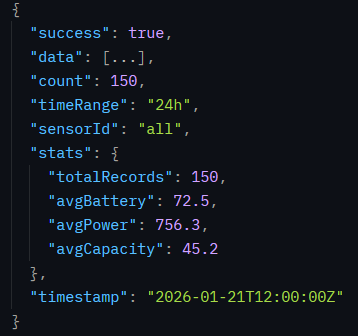
\includegraphics[width=0.65\textwidth]{images/api-response.png}
  % RENAME: image14.png → api-response.png
\end{figure}

\textit{Response} API mencakup data sensor, jumlah \textit{record}, serta statistik agregat yang dihitung langsung di \textit{database} menggunakan fungsi SQL \texttt{AVG()} dan \texttt{COUNT()}.

\subsection{Implementasi Antarmuka}

Antarmuka \textit{dashboard} diimplementasikan sebagai komponen React pada file \texttt{src\allowbreak/components\allowbreak/Dashboard.tsx}. Komponen ini menggunakan React Hooks untuk manajemen \textit{state} dan \textit{side effects}. Tabel \ref{tab:state-variable} menyajikan \textit{state variable} yang digunakan.

\begin{table}[H]
  \caption{\textit{State Variable} Komponen \textit{Dashboard}}
  \label{tab:state-variable}
  \begin{tabularx}{\textwidth}{| l | l | X |}
    \hline
    \textbf{\textit{State Variable}} & \textbf{Tipe} & \textbf{Deskripsi} \\
    \hline
    \texttt{selectedSensor} & string & Menyimpan ID sensor yang dipilih atau ``all'' untuk semua sensor \\
    \hline
    \texttt{timerange} & string & Rentang waktu data yang ditampilkan (24h, 7d, 30d) \\
    \hline
    \texttt{sensorData} & SensorDataPoint[] & \textit{Array} data mentah dari sensor yang diterima dari API \\
    \hline
    \texttt{processedData} & any[] & Data yang telah diproses untuk visualisasi \textit{chart} \\
    \hline
    \texttt{sensorStats} & object & Statistik agregat untuk setiap sensor \\
    \hline
    \texttt{loading} & boolean & Status \textit{loading} saat \textit{fetching} data \\
    \hline
    \texttt{lastUpdate} & Date \textbar{} null & \textit{Timestamp} pembaruan data terakhir \\
    \hline
    \texttt{availableSensors} & Number[] & Daftar sensor ID yang tersedia untuk opsi \textit{dropdown} \\
    \hline
  \end{tabularx}
\end{table}

\textit{Dashboard} terdiri dari enam komponen utama sebagai berikut.

\begin{enumerate}
  \item \textbf{\textit{Header Section}}: menampilkan judul aplikasi, tombol \textit{refresh} manual, dan informasi \textit{timestamp} pembaruan terakhir.

  \item \textbf{\textit{Sensor Status Cards}}: menampilkan kartu status untuk setiap sensor aktif, mencakup ID sensor, status operasional (NORMAL, WARNING, atau CRITICAL), \textit{fill level} dengan \textit{progress bar} berwarna (hijau $\leq$70\%, kuning 71--85\%, merah $>$85\%), persentase baterai, konsumsi daya, \textit{topic} MQTT, dan \textit{timestamp} terakhir.

  \item \textbf{\textit{Control Panel}}: menyediakan \textit{dropdown} pemilihan sensor, \textit{dropdown} rentang waktu (Last 24 Hours, Last 7 Days, Last 30 Days), serta informasi jumlah \textit{data points} dan \textit{active sensors}.

  \item \textbf{Visualisasi Data}: dua \textit{chart} interaktif menggunakan Recharts: \textit{Waste Fill Level Trend} (\textit{line chart} tren kepenuhan) dan \textit{Battery \& Power Consumption} (\textit{dual-axis line chart} baterai dan konsumsi daya).

  \item \textbf{\textit{Recent Sensor Readings}}: tabel 10 pembacaan sensor terbaru dengan \textit{progress bar} mini dan \textit{status indicator} berwarna.

  \item \textbf{\textit{System Analytics}}: lima metrik agregat: Total Records, Active Sensors, Avg Battery, Avg Power, dan Critical Alerts.
\end{enumerate}

\textit{Dashboard} mengimplementasikan \textit{auto-refresh} setiap 30 detik menggunakan \texttt{useEffect} Hook dengan \texttt{setInterval} dan \textit{cleanup function} untuk mencegah \textit{memory leak}. Tampilan lengkap antarmuka \textit{dashboard} disajikan pada Lampiran B.

\subsection{\textit{Deployment Dashboard}}

\textit{Dashboard} di-\textit{deploy} menggunakan \textit{platform} Vercel melalui integrasi Git. Setiap \textit{push} ke \textit{branch} utama memicu proses \textit{build} dan \textit{deployment} secara otomatis (\textit{Continuous Deployment}). Tabel \ref{tab:impl-hosting} menyajikan spesifikasi \textit{hosting} yang digunakan.

\begin{table}[H]
  \caption{Spesifikasi \textit{Hosting Dashboard}}
  \label{tab:impl-hosting}
  \begin{tabularx}{\textwidth}{| l | X |}
    \hline
    \textbf{Aspek} & \textbf{Spesifikasi} \\
    \hline
    \textit{Platform} & Vercel (\textit{free tier}) \\
    \hline
    \textit{Framework Preset} & Next.js \\
    \hline
    \textit{Build Command} & \texttt{next build} \\
    \hline
    \textit{Output Directory} & \texttt{.next} \\
    \hline
    \textit{Deployment Method} & Git Integration (\textit{Continuous Deployment}) \\
    \hline
    Domain & Subdomain Vercel (\texttt{*.vercel.app}) \\
    \hline
  \end{tabularx}
\end{table}
% ==========================================
% BAB VI EVALUASI
% ==========================================
\cleardoublepage
\chapter{EVALUASI}
\label{chap:evaluasi}

Bab ini merupakan pelaksanaan fase demonstrasi dan evaluasi dalam metodologi \textit{Design Science Research} yang telah diuraikan pada Bab I. Setelah sistem pemantauan sampah berbasis \textit{Internet of Things} dirancang dan diimplementasikan pada Bab IV dan V, tahap selanjutnya adalah mendemonstrasikan sistem di lapangan, mengevaluasi pemenuhannya terhadap kebutuhan yang telah ditetapkan, dan menganalisis data yang dikumpulkan untuk menjawab rumusan masalah penelitian.

% ============================================================
\section{Metode Evaluasi}
\label{sec:metode-evaluasi}
% ============================================================

Evaluasi sistem pemantauan sampah berbasis \textit{Internet of Things} dilakukan secara sistematis melalui beberapa skenario yang masing-masing dirancang untuk menjawab rumusan masalah yang telah ditetapkan pada Bab I. Sebelum menjelaskan skenario evaluasi, subbab ini terlebih dahulu mendeskripsikan konfigurasi sistem dan lingkungan pengujian yang digunakan selama periode evaluasi.

\subsection{Konfigurasi Pengujian Sistem}

Pengujian sistem dilakukan dengan mengoperasikan tiga unit perangkat \textit{Smart Waste Bin} di Lantai 4 Gedung Labtek VIII Institut Teknologi Bandung. Perangkat ditempatkan di area koridor depan Laboratorium IoT. Pemilihan lokasi ini didasarkan pada beberapa pertimbangan.

\begin{enumerate}
  \item Penempatan tiga unit tempat sampah berukuran besar di area umum gedung memerlukan proses perizinan yang panjang. Area depan Laboratorium IoT memungkinkan proses perizinan yang lebih sederhana dengan dukungan dari pengelola laboratorium.
  \item Peneliti sering beraktivitas di Laboratorium IoT, sehingga memudahkan \textit{monitoring} rutin dan \textit{maintenance} perangkat jika diperlukan.
  \item Meskipun berada di ujung lantai, area ini tetap dilalui oleh pengguna gedung dan memiliki aktivitas pembuangan sampah yang dapat diobservasi.
\end{enumerate}

Setiap unit \textit{smart waste bin} diberi kode warna sesuai dengan jenis sampah yang ditampung sebagaimana disajikan pada Tabel \ref{tab:detail-unit-swb}.

% Konten pendek & seragam → tabular + \centering
\begin{table}[H]
  \caption{Detail Unit \textit{Smart Waste Bin}}
  \label{tab:detail-unit-swb}
  \centering
  \begin{tabular}{| l | l | l | l |}
    \hline
    \textbf{Sensor ID} & \textbf{Kode Warna} & \textbf{Jenis Sampah} & \textbf{MQTT \textit{Topic}} \\
    \hline
    1 & Hijau  & Organik   & \texttt{wp2/basic\_01} \\
    \hline
    2 & Kuning & Anorganik & \texttt{wp2/basic\_02} \\
    \hline
    3 & Hitam  & Residu    & \texttt{wp2/basic\_03} \\
    \hline
  \end{tabular}
\end{table}

Konfigurasi pengujian mencakup seluruh komponen sistem dari \textit{Perception Layer} hingga \textit{Application Layer}. Tabel \ref{tab:konfigurasi-lingkungan} menyajikan konfigurasi lingkungan pengujian secara keseluruhan.

% Kolom kanan perlu wrap → tabularx + X
\begin{table}[H]
  \caption{Konfigurasi Lingkungan Pengujian}
  \label{tab:konfigurasi-lingkungan}
  \begin{tabularx}{\textwidth}{| l | X |}
    \hline
    \textbf{Aspek} & \textbf{Spesifikasi} \\
    \hline
    Lokasi & Lantai 4, Gedung Labtek VIII ITB \\
    \hline
    Area Penempatan & Koridor depan Laboratorium IoT \\
    \hline
    Jumlah Perangkat & 3 unit \\
    \hline
    Periode Pengumpulan Data & 24 Desember 2025 -- 29 Januari 2026 \\
    \hline
    Interval Pengiriman Data & $\pm$2,5 jam \\
    \hline
    Konektivitas & GSM/GPRS (SIM800L) \\
    \hline
    \textit{Database} & Supabase PostgreSQL \\
    \hline
    \textit{Dashboard} & Next.js pada Vercel \\
    \hline
  \end{tabularx}
\end{table}

\subsection{Skenario Evaluasi}

Skenario evaluasi dirancang untuk menjawab setiap rumusan masalah yang telah ditetapkan pada Bab I. Tabel \ref{tab:mapping-skenario} menyajikan \textit{mapping} antara rumusan masalah, skenario evaluasi, dan tujuan evaluasi.

% Semua kolom berisi teks panjang → tabularx + X
\begin{table}[H]
  \caption{\textit{Mapping} Rumusan Masalah dengan Skenario Evaluasi}
  \label{tab:mapping-skenario}
  \begin{tabularx}{\textwidth}{| l | X | X | X |}
    \hline
    \textbf{ID} & \textbf{Rumusan Masalah} & \textbf{Skenario Evaluasi} & \textbf{Tujuan Evaluasi} \\
    \hline
    RM-1 & Rancangan dan implementasi sistem pemantauan sampah berbasis \textit{Internet of Things} (IoT) yang mampu mengumpulkan data secara periodik dan terstruktur & SE-01: Evaluasi Fungsionalitas Sistem & Memverifikasi fungsi sistem berjalan sesuai rancangan \\
    \hline
    RM-1 & & SE-02: Evaluasi Pengumpulan Data & Mengukur keberhasilan pengumpulan data periodik \\
    \hline
    RM-1 & & SE-04: Evaluasi Adaptasi \textit{Firmware} & Mengevaluasi efektivitas adaptasi \textit{firmware} terhadap keandalan sistem \\
    \hline
    RM-2 & Pola pembuangan sampah yang dapat diidentifikasi berdasarkan data sistem dan validasinya terhadap observasi lapangan & SE-03: Analisis Pola Pembuangan & Mengidentifikasi pola temporal dan validasi lapangan \\
    \hline
  \end{tabularx}
\end{table}

\subsection{Metode Analisis Data}
\label{sec:metode-analisis-data}

Untuk menjawab RM-2, data yang terkumpul dianalisis menggunakan kombinasi metode analisis statistik deskriptif dan analisis temporal. Metode analisis ditetapkan terlebih dahulu sebelum pelaksanaan analisis agar proses identifikasi pola bersifat sistematis dan dapat ditelusuri. Tahapan dan metode analisis yang digunakan adalah sebagai berikut:

\begin{enumerate}
    \item \textbf{Praproses dan Pembersihan Data}

    Data mentah hasil pengumpulan terlebih dahulu disaring untuk membuang data kotor (\textit{dirty data}) yang melanggar batas fisik yang valid, seperti nilai \textit{fillLevel} di luar rentang 0--100\% atau nilai baterai yang tidak wajar. Kriteria pembersihan ditetapkan berdasarkan batas operasional yang mustahil dicapai secara fisik, sehingga tidak ada data valid yang terbuang.

    \item \textbf{Analisis Statistik Deskriptif}

    Statistik deskriptif (nilai rata-rata, standar deviasi, nilai minimum dan maksimum, serta distribusi) dihitung untuk setiap sensor guna memberikan gambaran umum karakteristik data yang terkumpul, termasuk sebaran \textit{fillLevel} dan profil konsumsi daya.

    \item \textbf{Analisis Delta (Deteksi \textit{Event} Penambahan)}

    Karena fokus analisis adalah aktivitas pembuangan, dilakukan analisis delta, yaitu menghitung selisih nilai \textit{fillLevel} antar pembacaan berurutan. Selisih positif yang melampaui ambang tertentu diidentifikasi sebagai \textit{event} penambahan sampah. Pendekatan berbasis \textit{event} ini dipilih karena lebih relevan untuk menangkap perilaku pembuangan dibandingkan nilai \textit{fillLevel} absolut.

    \item \textbf{Analisis Temporal}

    \textit{Event} penambahan yang teridentifikasi kemudian dipetakan terhadap dimensi waktu (jam, hari, hari kerja vs akhir pekan, serta hari libur) untuk mengidentifikasi pola temporal, seperti jam puncak (\textit{peak hour}) dan rentang jam aktif.

    \item \textbf{Analisis Komparatif Antar Jenis Sampah}

    Distribusi \textit{event} dan kontribusi volume dibandingkan antar tiga jenis sampah (organik, anorganik, residu) untuk mengidentifikasi karakteristik dominasi jenis sampah.

    \item \textbf{Validasi terhadap Observasi Lapangan}

    Pola yang teridentifikasi dari data divalidasi kewajarannya melalui observasi langsung di lokasi penelitian, untuk memastikan pola yang ditemukan konsisten dengan kondisi aktual aktivitas di lapangan.
\end{enumerate}

Perlu ditegaskan bahwa proses analisis ini dilakukan oleh peneliti terhadap data yang telah dikumpulkan oleh sistem. Sistem berperan sebagai instrumen pengumpul dan penyaji data, sedangkan identifikasi pola merupakan hasil analisis yang dilakukan secara terpisah dari operasional sistem.

% ============================================================
\section{Hasil Evaluasi}
\label{sec:hasil-evaluasi}
% ============================================================

Bagian ini menyajikan hasil evaluasi untuk setiap skenario yang telah dirancang pada Subbab \ref{sec:metode-evaluasi}. Setiap skenario dilengkapi dengan metodologi pengujian, hasil pengujian, dan kesimpulan yang menjawab rumusan masalah terkait.

\subsection{Hasil Evaluasi Fungsionalitas Sistem (SE-01)}

Skenario SE-01 mengevaluasi fungsionalitas seluruh komponen sistem pemantauan sampah berbasis \textit{Internet of Things} untuk memverifikasi bahwa arsitektur dan mekanisme berfungsi sesuai dengan desain pada Bab IV. Pengujian fungsionalitas dilakukan dengan metode \textit{black-box testing} pada setiap \textit{layer} arsitektur IoT.

Tabel \ref{tab:pengujian-fungsionalitas} menyajikan komponen, aspek pengujian, dan kriteria keberhasilan untuk setiap \textit{layer}.

% Aspek & kriteria perlu wrap → tabularx + X
\begin{table}[H]
  \caption{Pengujian Fungsionalitas Sistem}
  \label{tab:pengujian-fungsionalitas}
  \begin{tabularx}{\textwidth}{| l | l | X | X |}
    \hline
    \textbf{\textit{Layer}} & \textbf{Komponen} & \textbf{Aspek Pengujian} & \textbf{Kriteria Keberhasilan} \\
    \hline
    \textit{Perception} & VL53L0X & Pengukuran jarak objek & Persentase \textit{fillLevel} sesuai dengan persentase aktual \\
    \hline
    \textit{Perception} & INA219 & \textit{Monitoring} tegangan dan arus & Nilai dalam \textit{range} operasional normal; kegagalan $\leq$1 hari berturut-turut \\
    \hline
    \textit{Network} & SIM800L & Koneksi GPRS ke jaringan & Berhasil terhubung ke APN \textit{operator} \\
    \hline
    \textit{Network} & MQTT & \textit{Publish} data ke \textit{broker} & Data terkirim dengan format valid \\
    \hline
    \textit{Middleware} & Node-RED & \textit{Response endpoint} & Status 200 dengan data valid \\
    \hline
    \textit{Application} & \textit{Dashboard} & \textit{Rendering} komponen UI & Data ditampilkan dengan benar dan lengkap \\
    \hline
    \textit{Application} & Supabase & \textit{Insert} dan \textit{query} data & Data tersimpan dengan benar \\
    \hline
  \end{tabularx}
\end{table}

\subsubsection{Hasil Pengujian \textit{Perception Layer}}

Pengujian sensor VL53L0X dilakukan dengan membandingkan pembacaan sensor dengan pengukuran manual menggunakan meteran pada berbagai jarak, sebanyak 5 kali untuk setiap titik jarak. Tabel \ref{tab:hasil-vlx} menyajikan hasilnya.

% 3 kolom medium → tabularx + X merata
\begin{table}[H]
  \caption{Hasil Pengujian Sensor VL53L0X}
  \label{tab:hasil-vlx}
  \begin{tabularx}{\textwidth}{| X | X | X |}
    \hline
    \textbf{Jarak Aktual (cm, \textit{fillLevel} \%)} & \textbf{Pembacaan Sensor (\textit{raw})} & \textbf{Pembacaan Sensor (\textit{fillLevel})} \\
    \hline
    100 ($\sim$0\%)  & Sensor 1--3: $>$900   & Sensor 1--3: 0\%   \\
    \hline
    80 ($\sim$20\%)  & Sensor 1--3: 700--799 & Sensor 1--3: 20\%  \\
    \hline
    60 ($\sim$40\%)  & Sensor 1--3: 500--599 & Sensor 1--3: 40\%  \\
    \hline
    20 ($\sim$80\%)  & Sensor 1--3: 100--199 & Sensor 1--3: 80\%  \\
    \hline
    0 ($\sim$100\%)  & Sensor 1--3: 0--99    & Sensor 1--3: 100\% \\
    \hline
  \end{tabularx}
\end{table}

Penggunaan tipe data integer menyebabkan pembulatan (\textit{truncation}) yang memberikan efek stabilisasi pada indikator \textit{dashboard} agar tidak terlalu fluktuatif. Hasil pengujian menunjukkan kesesuaian yang tinggi antara pengukuran manual dengan \textit{output} sistem.

Pengujian sensor INA219 dilakukan selama periode pengumpulan data untuk memverifikasi keandalan pembacaan tegangan, arus, dan daya. Tabel \ref{tab:hasil-ina219} menyajikan hasilnya.

% 6 kolom pendek → tabular + \centering
\begin{table}[H]
  \caption{Hasil Pengujian Sensor INA219}
  \label{tab:hasil-ina219}
  \centering
  \begin{tabular}{| l | l | l | l | l | l |}
    \hline
    \textbf{Sensor} & \textbf{Jenis} & \textbf{Tegangan (V)} & \textbf{Arus (mA)} & \textbf{Daya (mW)} & \textbf{Status} \\
    \hline
    1 & Organik   & 7,30--7,50 & 110--140 & 803--1.050   & OK \\
    \hline
    2 & Anorganik & 7,10--7,45 & 110--135 & 781--1.006   & OK \\
    \hline
    3 & Residu    & 6,90--7,50 & 210--235 & 1.449--1.763 & FAILED \\
    \hline
  \end{tabular}
\end{table}

Sensor 3 (Residu) menunjukkan konsumsi arus hampir dua kali lipat (210--235 mA) dibandingkan sensor lainnya (110--140 mA). Sensor 3 juga mengalami kegagalan INA219 selama 4 hari berturut-turut (11--14 Januari 2026), melebihi batas kriteria 1 hari berturut-turut. Kegagalan ini bertepatan dengan gangguan kabel I2C yang juga menyebabkan kegagalan VL53L0X secara bersamaan. Setelah perbaikan kabel, pembacaan kembali normal.

\subsubsection{Hasil Pengujian \textit{Network Layer}}

Pengujian \textit{Network Layer} dilakukan sebelum pemasangan perangkat dengan memverifikasi \textit{output debug} pada \textit{Serial Monitor}. Tabel \ref{tab:hasil-gprs} menyajikan hasil pengujian modem GPRS.

% Kolom tengah perlu wrap → tabularx
\begin{table}[H]
  \caption{Hasil Pengujian Modem GPRS}
  \label{tab:hasil-gprs}
  \begin{tabularx}{\textwidth}{| l | X | l |}
    \hline
    \textbf{Tahap} & \textbf{\textit{Output Serial Monitor}} & \textbf{Status} \\
    \hline
    Inisialisasi Modem  & Initializing modem\ldots           & OK \\
    \hline
    Info Modem          & Modem Info: SIM800 R14.18          & OK \\
    \hline
    Registrasi Jaringan & Waiting for network\ldots success  & OK \\
    \hline
    Koneksi APN         & Connecting to M2MINTERNET\ldots success & OK \\
    \hline
    Status GPRS         & GPRS connected                     & OK \\
    \hline
  \end{tabularx}
\end{table}

Pengujian MQTT dilakukan dalam dua tahap: menggunakan \textit{listener} lokal untuk memverifikasi data terkirim, kemudian menggunakan Node-RED sebagai \textit{subscriber}. Tabel \ref{tab:hasil-mqtt} menyajikan hasilnya.

% Kolom tengah perlu wrap → tabularx
\begin{table}[H]
  \caption{Hasil Pengujian MQTT}
  \label{tab:hasil-mqtt}
  \begin{tabularx}{\textwidth}{| l | X | l |}
    \hline
    \textbf{Tahap} & \textbf{Hasil} & \textbf{Status} \\
    \hline
    Koneksi ke \textit{Broker}   & Connecting to 38.47.176.109\ldots success & OK \\
    \hline
    Test \textit{Listener} Lokal & Data JSON diterima pada \textit{topic} \texttt{wp2/basic\_01}, \texttt{\_02}, \texttt{\_03} & OK \\
    \hline
    Test ke Node-RED             & Node-RED menerima dan mem-\textit{parse} data JSON dengan benar & OK \\
    \hline
    Format \textit{Payload}      & JSON valid dengan seluruh \textit{field} yang diperlukan & OK \\
    \hline
  \end{tabularx}
\end{table}

\subsubsection{Hasil Pengujian \textit{Middleware Layer} dan \textit{Application Layer}}

Pengujian \textit{Middleware Layer} memastikan setiap \textit{payload} MQTT berhasil ditangkap, di-\textit{parse}, dan disimpan ke \textit{database} tanpa \textit{data loss} atau \textit{corrupt}. Tabel \ref{tab:hasil-nodered} menyajikan hasilnya.

% Dua kolom pertama perlu wrap → tabularx
\begin{table}[H]
  \caption{Hasil Pengujian Node-RED}
  \label{tab:hasil-nodered}
  \begin{tabularx}{\textwidth}{| X | X | l |}
    \hline
    \textbf{Aspek Pengujian} & \textbf{Hasil} & \textbf{Status} \\
    \hline
    \textit{Subscribe} MQTT    & Berhasil \textit{subscribe} ke ketiga \textit{topic} & OK \\
    \hline
    \textit{Parsing} JSON      & Data di-\textit{parse} dengan benar menggunakan JSON \textit{node} & OK \\
    \hline
    \textit{Insert} ke Supabase & Data diteruskan ke Supabase melalui HTTP \textit{request} & OK \\
    \hline
    \textit{Data Integrity}    & Tidak ada data \textit{corrupt} atau duplikat & OK \\
    \hline
    \textit{Query Performance} & \textit{Response time} $<$500ms untuk \textit{query} 1 minggu & OK \\
    \hline
  \end{tabularx}
\end{table}

Pengujian API \textit{endpoint} dilakukan dengan \textit{request} HTTP GET menggunakan berbagai parameter \textit{filter}. Tabel \ref{tab:hasil-api} menyajikan hasilnya.

% Kolom endpoint panjang → tabularx, sisanya pendek → l
\begin{table}[H]
  \caption{Hasil Pengujian API \textit{Dashboard}}
  \label{tab:hasil-api}
  \begin{tabularx}{\textwidth}{| X | l | l | l | l |}
    \hline
    \textbf{\textit{Endpoint}} & \textbf{Method} & \textbf{Expected} & \textbf{Aktual} & \textbf{Status} \\
    \hline
    \texttt{/api/sensor-data}                   & GET & 200, array             & 200 & OK \\
    \hline
    \texttt{/api/sensor-data?sensorId=1}        & GET & 200, \textit{filtered} & 200 & OK \\
    \hline
    \texttt{/api/sensor-data?sensorId=2}        & GET & 200, \textit{filtered} & 200 & OK \\
    \hline
    \texttt{/api/sensor-data?sensorId=3}        & GET & 200, \textit{filtered} & 200 & OK \\
    \hline
    \texttt{/api/sensor-data?timerange=24h}     & GET & 200, 24h data          & 200 & OK \\
    \hline
    \texttt{/api/sensor-data?timerange=7d}      & GET & 200, 7d data           & 200 & OK \\
    \hline
  \end{tabularx}
\end{table}

Pengujian antarmuka \textit{dashboard} dilakukan secara \textit{end-to-end} untuk memverifikasi visualisasi dan fitur interaktif. Tabel \ref{tab:hasil-ui} menyajikan hasilnya.

% Kolom tengah perlu wrap → tabularx
\begin{table}[H]
  \caption{Hasil Pengujian Komponen \textit{Dashboard}}
  \label{tab:hasil-ui}
  \begin{tabularx}{\textwidth}{| l | X | l |}
    \hline
    \textbf{Komponen} & \textbf{Aspek Pengujian} & \textbf{Hasil} \\
    \hline
    \textit{Header Section}   & Menampilkan judul, tombol \textit{refresh}, \textit{last update} & Sesuai \\
    \hline
    \textit{Sensor Cards}     & Menampilkan status 3 sensor dengan warna \textit{threshold} & Sesuai \\
    \hline
    \textit{Fill Level} Bar   & \textit{Progress bar} sesuai persentase \textit{fillLevel} & Sesuai \\
    \hline
    \textit{Control Panel}    & \textit{Filter} sensor dan \textit{time range} berfungsi & Sesuai \\
    \hline
    Chart \textit{Fill Level} & \textit{Line chart} menampilkan tren \textit{fillLevel} & Sesuai \\
    \hline
    Chart \textit{Battery}    & \textit{Dual-axis chart} baterai dan \textit{power consumption} & Sesuai \\
    \hline
    \textit{Auto-refresh}     & Data ter-\textit{update} setiap 30 detik & Sesuai \\
    \hline
  \end{tabularx}
\end{table}

Seluruh komponen sistem dari \textit{Perception Layer} hingga \textit{Application Layer} berfungsi sesuai dengan desain. Hasil pengujian ini menjawab RM-1 terkait komponen, arsitektur, dan mekanisme sistem pemantauan sampah berbasis \textit{Internet of Things} (IoT).

\subsection{Hasil Evaluasi Pengumpulan Data (SE-02)}

Skenario SE-02 mengevaluasi keberhasilan dan konsistensi pengumpulan data secara periodik selama periode observasi.

\subsubsection{Periode Pengumpulan Data}

Tabel \ref{tab:detail-pengumpulan} menyajikan detail periode pengumpulan data.

% Kolom kanan perlu wrap → tabularx
\begin{table}[H]
  \caption{Detail Pengumpulan Data}
  \label{tab:detail-pengumpulan}
  \begin{tabularx}{\textwidth}{| l | X |}
    \hline
    \textbf{Aspek} & \textbf{Nilai} \\
    \hline
    Tanggal mulai & 24 Desember 2025 \\
    \hline
    Tanggal selesai & 29 Januari 2026 \\
    \hline
    Total durasi & 37 hari \\
    \hline
    Hari kerja (Senin--Jumat) & 24 hari \\
    \hline
    \textit{Weekend} (Sabtu--Minggu) & 10 hari \\
    \hline
    Hari libur nasional & 3 hari (25--26 Des 2025, 1 Jan 2026) \\
    \hline
    Target interval pengiriman & $\pm$2,5 jam (\texttt{TIME\_TO\_SLEEP} = 150 menit) \\
    \hline
  \end{tabularx}
\end{table}

\subsubsection{Volume Data Terkumpul}

Tabel \ref{tab:volume-data} menyajikan jumlah data yang berhasil dikumpulkan dari setiap sensor.

% 6 kolom pendek → tabular + \centering
\begin{table}[H]
  \caption{Jumlah Data Terkumpul per Sensor}
  \label{tab:volume-data}
  \centering
  \begin{tabular}{| l | l | l | l | l | l |}
    \hline
    \textbf{Sensor} & \textbf{Jenis} & \textbf{\textit{Records}} & \textbf{Target} & \textbf{Pencapaian} & \textbf{Status} \\
    \hline
    1     & Organik   & 289 & 296 & 97,6\% & OK \\
    \hline
    2     & Anorganik & 290 & 296 & 98,0\% & OK \\
    \hline
    3     & Residu    & 237 & 296 & 80,0\% & Sebagian OK \\
    \hline
    Total & --        & 816 & 888 & 91,9\% & -- \\
    \hline
  \end{tabular}
\end{table}

Target 296 \textit{records} per sensor diperoleh dari 37 hari $\times$ 8 \textit{records}/hari (interval 3 jam). Sensor 1 (Organik) dan Sensor 2 (Anorganik) mencapai target mendekati 100\%. Sensor 3 (Residu) mencapai 80,0\% yang lebih rendah karena konsumsi daya lebih tinggi (210--235 mA vs 110--140 mA) sehingga baterai lebih cepat habis. Dari 816 \textit{records} yang terkirim, 805 \textit{records} dinyatakan valid setelah \textit{filtering} data kotor.

\subsubsection{Konsistensi Interval Pengiriman}

Tabel \ref{tab:statistik-interval} menyajikan statistik interval pengiriman data untuk setiap sensor.

% 5 kolom pendek-medium → tabular + \centering
\begin{table}[H]
  \caption{Statistik Interval Pengiriman Data}
  \label{tab:statistik-interval}
  \centering
  \begin{tabular}{| l | l | l | l | l |}
    \hline
    \textbf{Sensor} & \textbf{Rata-rata} & \textbf{Minimum} & \textbf{Maksimum} & \textbf{Std Dev} \\
    \hline
    1 & 2 jam 24 menit & 35 menit & 4 jam 58 menit & 25 menit \\
    \hline
    2 & 2 jam 24 menit & 22 menit & 5 jam 22 menit & 31 menit \\
    \hline
    3 & 2 jam 21 menit & 2 menit* & 4 jam 57 menit & 38 menit \\
    \hline
  \end{tabular}
\end{table}

*Nilai minimum sangat kecil merupakan indikasi \textit{retry} pengiriman setelah koneksi gagal, bukan interval reguler. Rata-rata interval $\pm$144 menit ($\approx$2 jam 24 menit) mendekati target \texttt{TIME\_TO\_SLEEP} = 150 menit.

\subsubsection{Analisis \textit{Data Loss} dan Data Kotor}

Tabel \ref{tab:analisis-dataloss} menyajikan analisis penyebab \textit{data loss} selama periode pengumpulan.

% Kolom pertama & terakhir perlu wrap → tabularx
\begin{table}[H]
  \caption{Penyebab \textit{Data Loss} dan Data Kotor}
  \label{tab:analisis-dataloss}
  \begin{tabularx}{\textwidth}{| X | l | l | X |}
    \hline
    \textbf{Kategori} & \textbf{Jumlah} & \textbf{\%} & \textbf{Penyebab} \\
    \hline
    Data sukses terkirim & 816 & 91,9\% & -- \\
    \hline
    Baterai habis/bocor & 64 & 7,2\% & \textit{Deep sleep} karena baterai habis; 4 baterai bocor (mati total), terutama pada Sensor 3 \\
    \hline
    MQTT \textit{broker} \textit{down} & 8 & 0,9\% & \textit{Broker} dimatikan pihak ketiga; pengumpulan dihentikan 29 Januari 2026 \\
    \hline
    \textbf{Total \textit{data loss}} & \textbf{72} & \textbf{8,1\%} & Dalam batas toleransi ($<$10\%) \\
    \hline
  \end{tabularx}
\end{table}

Selain \textit{data loss}, terdapat data yang berhasil terkirim namun memiliki nilai tidak valid. Tabel \ref{tab:jenis-data-kotor} menyajikan jenis-jenis data kotor yang teridentifikasi.

% Kolom indikator & penyebab panjang → tabularx
\begin{table}[H]
  \caption{Jenis-jenis Data Kotor}
  \label{tab:jenis-data-kotor}
  \begin{tabularx}{\textwidth}{| l | l | X | X |}
    \hline
    \textbf{Jenis Anomali} & \textbf{Jumlah} & \textbf{Indikator} & \textbf{Penyebab} \\
    \hline
    \textit{Battery} 999\% & 7 & tegangan = arus = batt = 999, \textit{fillLevel} = -1, \texttt{ina219\_avail} = 0, \texttt{vl53l0x\_avail} = 0 & Kabel I2C putus total; seluruhnya dari Sensor 3 \\
    \hline
    \textit{fillLevel} = -1 atau $>$100 & 3 & \textit{fillLevel} di luar 0--100\% & VL53L0X \textit{timeout} atau \textit{error} \\
    \hline
  \end{tabularx}
\end{table}

Dari 816 \textit{records} yang terkirim, terdapat 11 \textit{record} kotor (1,3\%) yang seluruhnya berasal dari Sensor 3 (Residu), disebabkan oleh masalah kabel I2C yang konsisten dengan anomali konsumsi daya tinggi pada unit tersebut. Setelah \textit{filtering}, tersisa 805 \textit{records} bersih. Data kotor dapat diidentifikasi melalui kolom \texttt{vl53l0x\_avail} dan \texttt{ina219\_avail}.

\subsubsection{Kualitas Data Setelah \textit{Filtering}}

Tabel \ref{tab:kualitas-data} menyajikan hasil analisis kualitas data setelah \textit{filtering} berdasarkan kolom \textit{availability} sensor.

% Kolom pertama panjang → tabularx + X
\begin{table}[H]
  \caption{Hasil Kualitas Data Setelah \textit{Filtering}}
  \label{tab:kualitas-data}
  \begin{tabularx}{\textwidth}{| X | l |}
    \hline
    \textbf{Metrik Kualitas} & \textbf{Hasil} \\
    \hline
    \multicolumn{2}{|l|}{\textit{Sebelum filter}: 816 \textit{records} \quad \textit{Setelah filter}: 805 \textit{records} (98,7\%)} \\
    \hline
    Data dengan \texttt{vl53l0x\_avail} = 1 (sensor jarak aktif) & 100\% \\
    \hline
    Data dengan \texttt{ina219\_avail} = 1 (sensor daya aktif) & 100\% \\
    \hline
    \textit{fillLevel} dalam \textit{range} valid (0--100\%) setelah \textit{filter} & 100\% \\
    \hline
    \textit{Timestamp} valid (format ISO 8601, \textit{timezone} Asia/Jakarta) & 100\% \\
    \hline
    Tidak ada duplikat (unique \textit{timestamp} + \texttt{sensor\_id}) & 100\% \\
    \hline
    \textit{Battery percentage} dalam \textit{range} valid (0--100\%) & 100\% \\
    \hline
    \texttt{sensor\_id} valid (1, 2, atau 3) & 100\% \\
    \hline
  \end{tabularx}
\end{table}

Kualitas data yang terkumpul sangat baik dengan validitas 100\% untuk semua metrik setelah \textit{filtering}. Data dengan \texttt{vl53l0x\_avail} = 0 atau \texttt{ina219\_avail} = 0 di-\textit{filter} pada tahap \textit{preprocessing} sebelum analisis pola.

\subsubsection{Distribusi Temporal Data}

Tabel \ref{tab:distribusi-jam} dan Tabel \ref{tab:distribusi-hari} menyajikan distribusi data berdasarkan waktu untuk memastikan data terdistribusi merata.

% 3 kolom pendek → tabular + \centering
\begin{table}[H]
  \caption{Jumlah \textit{Record} per Rentang Jam}
  \label{tab:distribusi-jam}
  \centering
  \begin{tabular}{| l | l | l |}
    \hline
    \textbf{Rentang Jam} & \textbf{Jumlah \textit{Records}} & \textbf{Persentase} \\
    \hline
    07:00--09:00        & 56  & 7,0\%  \\
    \hline
    09:00--12:00        & 81  & 10,1\% \\
    \hline
    12:00--14:00        & 53  & 6,6\%  \\
    \hline
    14:00--17:00        & 119 & 14,8\% \\
    \hline
    17:00--19:00        & 73  & 9,1\%  \\
    \hline
    19:00--07:00        & 423 & 52,5\% \\
    \hline
    \textbf{Total}      & \textbf{805} & \textbf{100\%} \\
    \hline
  \end{tabular}
\end{table}

% 3 kolom pendek → tabular + \centering
\begin{table}[H]
  \caption{Jumlah \textit{Record} per Hari}
  \label{tab:distribusi-hari}
  \centering
  \begin{tabular}{| l | l | l |}
    \hline
    \textbf{Hari} & \textbf{Jumlah \textit{Records}} & \textbf{Persentase} \\
    \hline
    Senin         & 102 & 12,7\% \\
    \hline
    Selasa        & 127 & 15,8\% \\
    \hline
    Rabu          & 153 & 19,0\% \\
    \hline
    Kamis         & 135 & 16,8\% \\
    \hline
    Jumat         & 108 & 13,4\% \\
    \hline
    Sabtu         & 91  & 11,3\% \\
    \hline
    Minggu        & 89  & 11,1\% \\
    \hline
    \textbf{Total} & \textbf{805} & \textbf{100\%} \\
    \hline
  \end{tabular}
\end{table}

Rentang 19:00--07:00 mendominasi distribusi jam (52,5\%) karena sensor mengirim data setiap $\pm$2,5 jam selama 24 jam penuh termasuk malam hari. Dari 805 \textit{records}, sebanyak 382 \textit{records} (47,5\%) berasal dari jam aktif kampus (07:00--19:00). Distribusi per hari relatif merata dengan hari kerja (Senin--Jumat) masing-masing berkontribusi 12--19\%, sedangkan Sabtu dan Minggu masing-masing 11,3\% dan 11,1\%.

\subsection{Hasil Analisis Pola Pembuangan Sampah (SE-03)}

Skenario SE-03 mengidentifikasi pola temporal pembuangan sampah berdasarkan data yang dikumpulkan dan memvalidasinya dengan observasi lapangan untuk menjawab RM-2. Analisis dilakukan menggunakan \textit{script} Python yang mencakup \textit{data cleaning}, perhitungan statistik deskriptif, dan visualisasi pola (kode sumber tersedia pada Lampiran A).

\subsubsection{Statistik Deskriptif \textit{fillLevel}}

Tabel \ref{tab:statistik-filllevel} menyajikan statistik deskriptif \textit{fillLevel} untuk setiap sensor selama periode observasi.

\begin{table}[H]
  \caption{Statistik Deskriptif \textit{fillLevel} per Sensor}
  \label{tab:statistik-filllevel}
  \centering
  \begin{tabular}{| l | l | l | l |}
    \hline
    \textbf{Statistik} & \textbf{Organik (S1)} & \textbf{Anorganik (S2)} & \textbf{Residu (S3)} \\
    \hline
    Jumlah data (n) & 289    & 290    & 226 \\
    \hline
    \textit{Mean}   & 5,3\%  & 14,4\% & 6,4\% \\
    \hline
    Median          & 0\%    & 10\%   & 10\% \\
    \hline
    Modus           & 0\%    & 0\%    & 10\% \\
    \hline
    Std Deviasi     & 5,7\%  & 13,0\% & 6,0\% \\
    \hline
    Minimum         & 0\%    & 0\%    & 0\% \\
    \hline
    Maksimum        & 20\%   & 40\%   & 20\% \\
    \hline
  \end{tabular}
\end{table}

\begin{figure}[H]
  \caption{Statistik \textit{fillLevel} per Sensor}
  \label{fig:statistik-filllevel}
  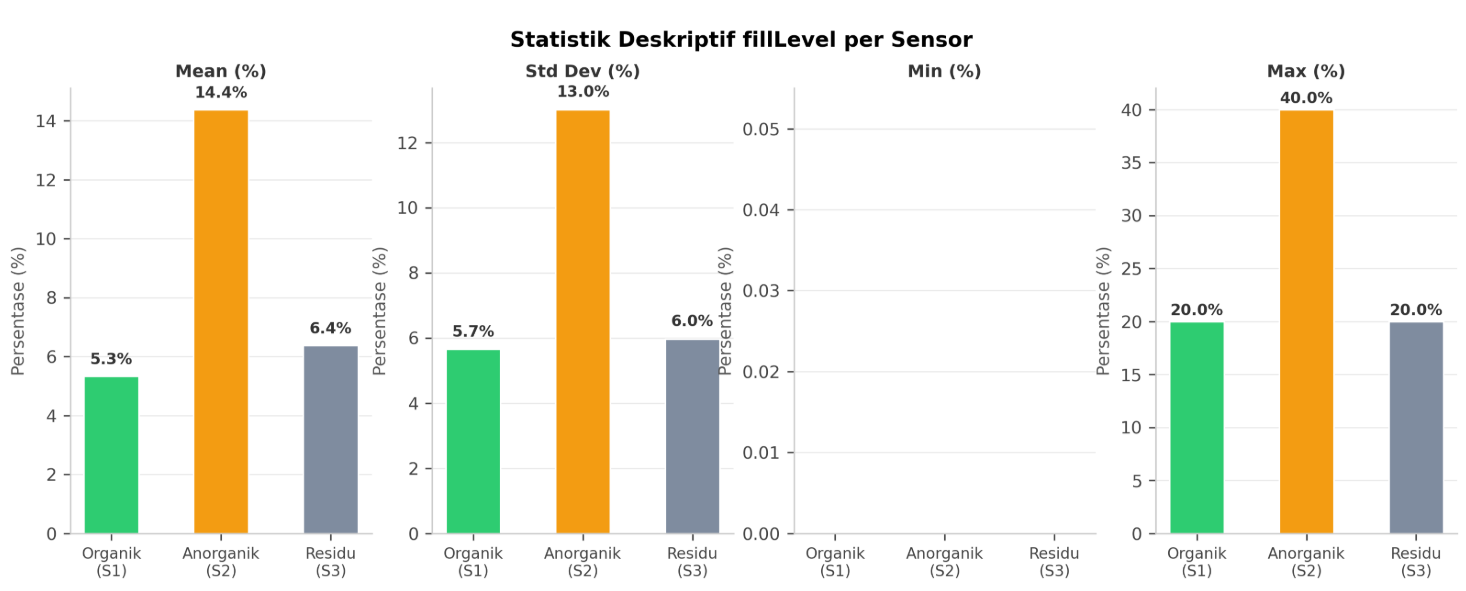
\includegraphics[width=\textwidth]{images/statistik-filllevel.png}
  % RENAME: image15.png → statistik-filllevel.png
\end{figure}

Sensor 2 (Anorganik) memiliki rata-rata \textit{fillLevel} tertinggi (14,4\%) dengan variasi terbesar (std 13,0\%), menunjukkan aktivitas pembuangan sampah anorganik paling tinggi di lokasi pengujian, sebagaimana divisualisasikan pada Gambar \ref{fig:statistik-filllevel}. Median Organik (S1) bernilai 0\% karena lebih dari separuh \textit{records} memiliki \textit{fillLevel} 0\%, mencerminkan frekuensi pengosongan yang tinggi.

\subsubsection{Distribusi \textit{fillLevel}}

Tabel \ref{tab:distribusi-filllevel} menyajikan distribusi frekuensi nilai \textit{fillLevel} pada setiap sensor.

\begin{table}[H]
  \caption{Distribusi \textit{fillLevel} per Sensor}
  \label{tab:distribusi-filllevel}
  \centering
  \begin{tabular}{| l | l | l | l |}
    \hline
    \textbf{\textit{fillLevel}} & \textbf{Organik (S1)} & \textbf{Anorganik (S2)} & \textbf{Residu (S3)} \\
    \hline
    0\%  & 145 (50,2\%) & 93 (32,1\%)  & 96 (42,5\%) \\
    \hline
    10\% & 134 (46,4\%) & 66 (22,8\%)  & 116 (51,3\%) \\
    \hline
    20\% & 10 (3,5\%)   & 69 (23,8\%)  & 14 (6,2\%) \\
    \hline
    30\% & 0 (0\%)      & 35 (12,1\%)  & 0 (0\%) \\
    \hline
    40\% & 0 (0\%)      & 27 (9,3\%)   & 0 (0\%) \\
    \hline
  \end{tabular}
\end{table}

Sampah Anorganik memiliki distribusi \textit{fillLevel} paling bervariasi dengan nilai mencapai 40\%, sedangkan Organik dan Residu didominasi oleh \textit{fillLevel} rendah (0--10\%) yang menunjukkan tempat sampah dikosongkan secara rutin.

\subsubsection{Pola Temporal Harian}

Analisis pola harian dilakukan dengan mengelompokkan rata-rata \textit{fillLevel} berdasarkan rentang jam, sebagaimana disajikan pada Tabel \ref{tab:pola-harian} dan divisualisasikan pada Gambar \ref{fig:pola-harian}. Nilai yang ditampilkan merupakan rata-rata \textit{fillLevel} kumulatif per slot waktu, bukan laju penambahan.

\begin{table}[H]
  \caption{Pola Temporal Harian}
  \label{tab:pola-harian}
  \begin{tabularx}{\textwidth}{| l | l | l | l | X |}
    \hline
    \textbf{Rentang Jam} & \textbf{Organik} & \textbf{Anorganik} & \textbf{Residu} & \textbf{Keterangan} \\
    \hline
    07:00--09:00 & 6,5\%  & 11,4\% & 5,7\%  & Awal aktivitas kampus \\
    \hline
    09:00--12:00 & 5,9\%  & 14,8\% & 8,8\%  & Jam kerja/kuliah pagi \\
    \hline
    12:00--14:00 & 7,8\%  & 13,2\% & 10,0\% & Jam makan siang \\
    \hline
    14:00--17:00 & 5,6\%  & 13,4\% & 5,7\%  & Jam kerja/kuliah sore \\
    \hline
    17:00--19:00 & 5,6\%  & 15,7\% & 5,5\%  & Akhir aktivitas \\
    \hline
    19:00--07:00 & 4,7\%  & 14,9\% & 5,8\%  & Non-aktif (malam) \\
    \hline
  \end{tabularx}
\end{table}

\begin{figure}[H]
  \caption{Distribusi \textit{fillLevel} per Rentang Jam}
  \label{fig:pola-harian}
  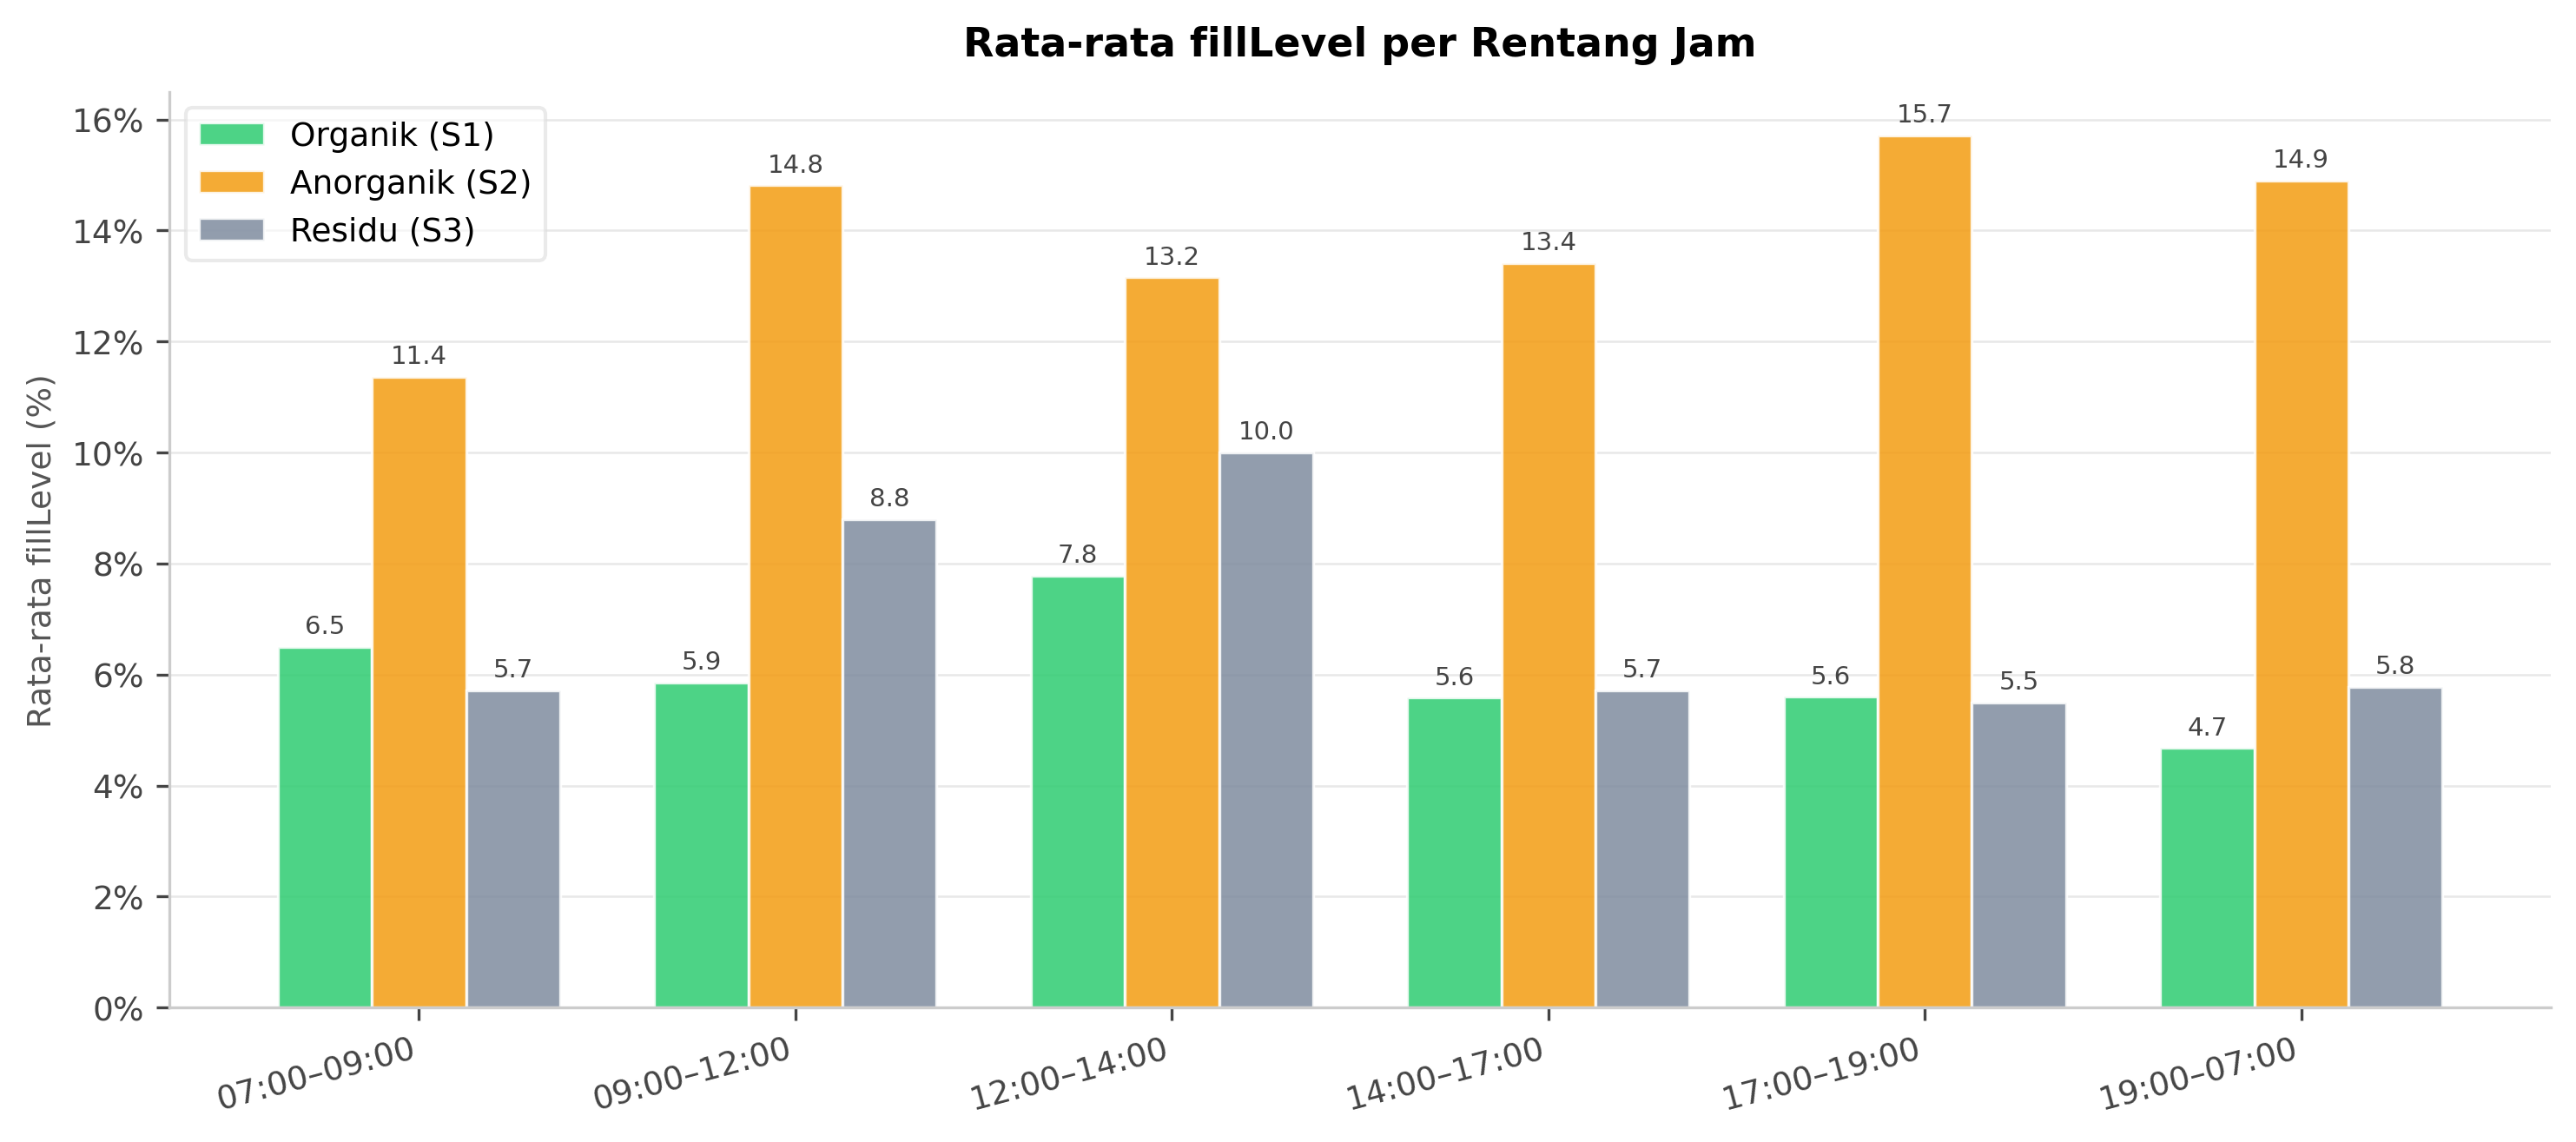
\includegraphics[width=\textwidth]{images/pola-harian.png}
  % RENAME: image16.png → pola-harian.png
\end{figure}

Nilai \textit{fillLevel} tertinggi pada S1 (Organik) dan S3 (Residu) terjadi pada rentang 12:00--14:00, konsisten dengan aktivitas makan siang. S2 (Anorganik) menunjukkan \textit{fillLevel} relatif tinggi dan merata sepanjang hari.

\subsubsection{Pola Temporal Mingguan}

Analisis pola mingguan dilakukan dengan mengelompokkan rata-rata \textit{fillLevel} berdasarkan hari, sebagaimana disajikan pada Tabel \ref{tab:pola-mingguan} dan divisualisasikan pada Gambar \ref{fig:pola-mingguan}. Nilai \textit{fillLevel} bersifat kumulatif antar pengosongan sehingga pola dipengaruhi jadwal pengosongan aktual, bukan semata aktivitas pengguna.

\begin{table}[H]
  \caption{Pola Temporal Mingguan}
  \label{tab:pola-mingguan}
  \centering
  \begin{tabular}{| l | l | l | l | l |}
    \hline
    \textbf{Hari} & \textbf{Organik} & \textbf{Anorganik} & \textbf{Residu} & \textbf{Kategori} \\
    \hline
    Senin  & 5,0\% & 10,8\% & 8,9\% & Hari kerja \\
    \hline
    Selasa & 7,2\% & 13,0\% & 8,0\% & Hari kerja \\
    \hline
    Rabu   & 4,7\% & 14,1\% & 8,9\% & Hari kerja \\
    \hline
    Kamis  & 4,0\% & 15,3\% & 5,3\% & Hari kerja \\
    \hline
    Jumat  & 5,0\% & 16,7\% & 0,6\% & Hari kerja \\
    \hline
    Sabtu  & 5,6\% & 18,5\% & 3,9\% & \textit{Weekend} \\
    \hline
    Minggu & 6,2\% & 12,5\% & 7,6\% & \textit{Weekend} \\
    \hline
  \end{tabular}
\end{table}

\begin{figure}[H]
  \caption{Rata-rata \textit{fillLevel} per Hari dalam Seminggu}
  \label{fig:pola-mingguan}
  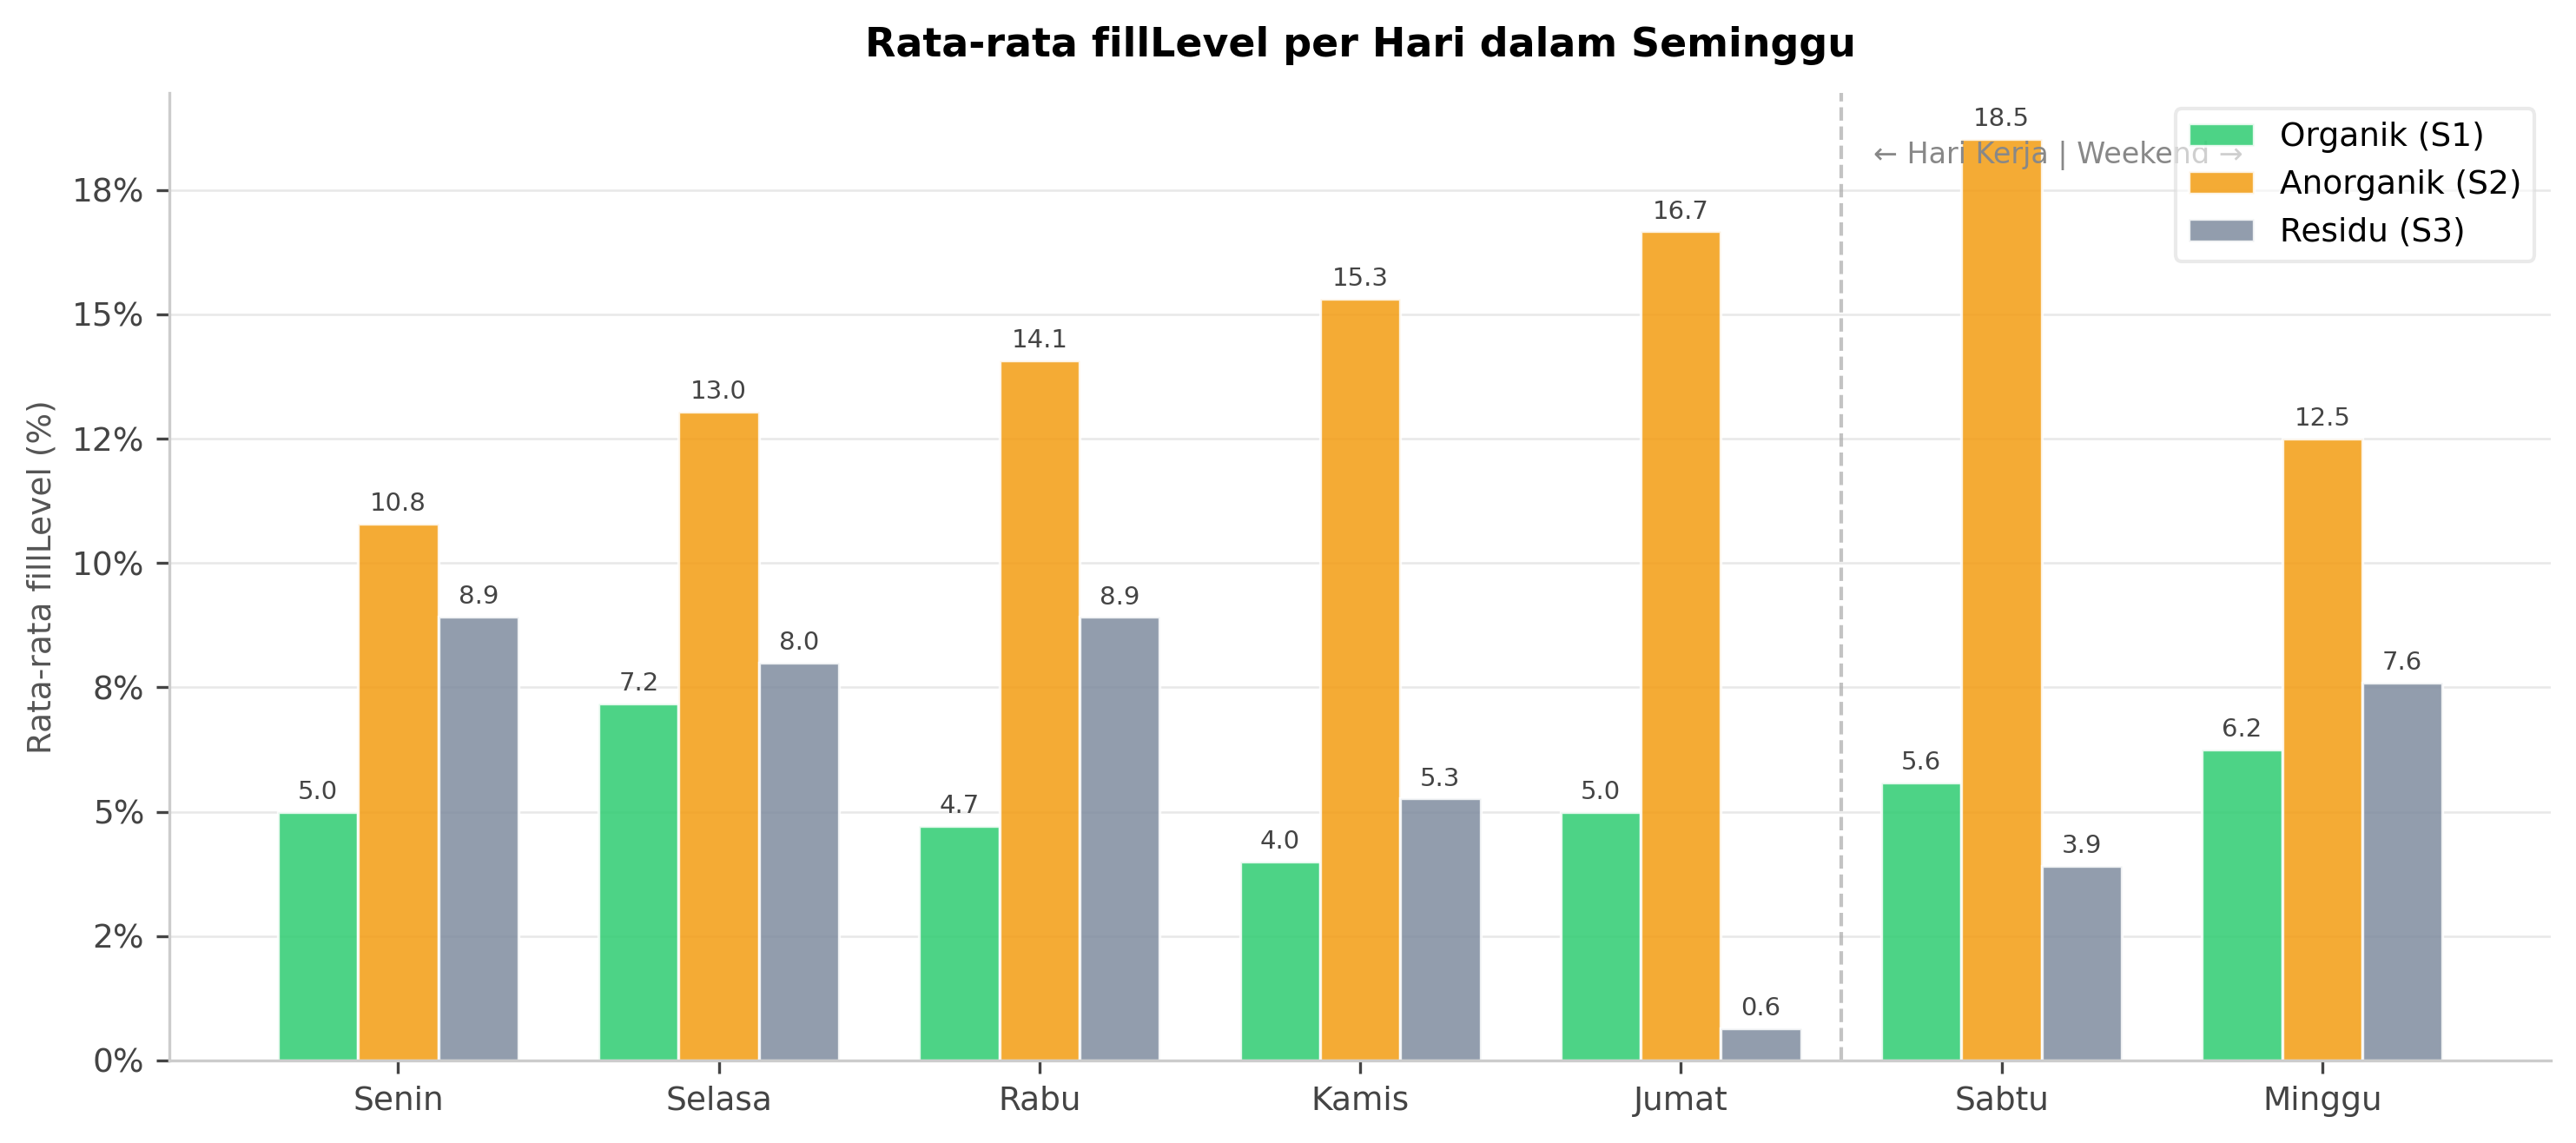
\includegraphics[width=\textwidth]{images/pola-mingguan.png}
  % RENAME: image17.png → pola-mingguan.png
\end{figure}

Rata-rata hari kerja: 5,2\% (Organik), 14,0\% (Anorganik), 6,3\% (Residu). Rata-rata \textit{weekend}: 5,9\% (Organik), 15,6\% (Anorganik), 5,8\% (Residu). Perbedaan antar hari kerja dan \textit{weekend} tidak signifikan karena \textit{fillLevel} bersifat kumulatif, sehingga nilai tinggi pada hari tertentu dapat mencerminkan akumulasi dari hari-hari sebelumnya sebelum terjadi pengosongan.

\subsubsection{Analisis Pengaruh Hari Libur}

Tabel \ref{tab:pola-libur} menyajikan rata-rata \textit{fillLevel} berdasarkan kategori hari, dan Gambar \ref{fig:pola-libur} memvisualisasikan perbandingannya.

\begin{table}[H]
  \caption{Pola Hari Libur}
  \label{tab:pola-libur}
  \centering
  \begin{tabular}{| l | l | l | l | l |}
    \hline
    \textbf{Kategori Hari} & \textbf{Organik} & \textbf{Anorganik} & \textbf{Residu} & \textbf{Jumlah Hari} \\
    \hline
    Hari kerja (Senin--Jumat) & 5,1\%  & 13,6\% & 6,9\% & 24 hari \\
    \hline
    \textit{Weekend} (Sabtu--Minggu) & 5,9\% & 15,6\% & 5,8\% & 10 hari \\
    \hline
    Hari libur nasional & 5,5\% & 18,0\% & 3,5\% & 3 hari \\
    \hline
  \end{tabular}
\end{table}

\begin{figure}[H]
  \caption{Rata-rata \textit{fillLevel} Berdasarkan Kategori Hari}
  \label{fig:pola-libur}
  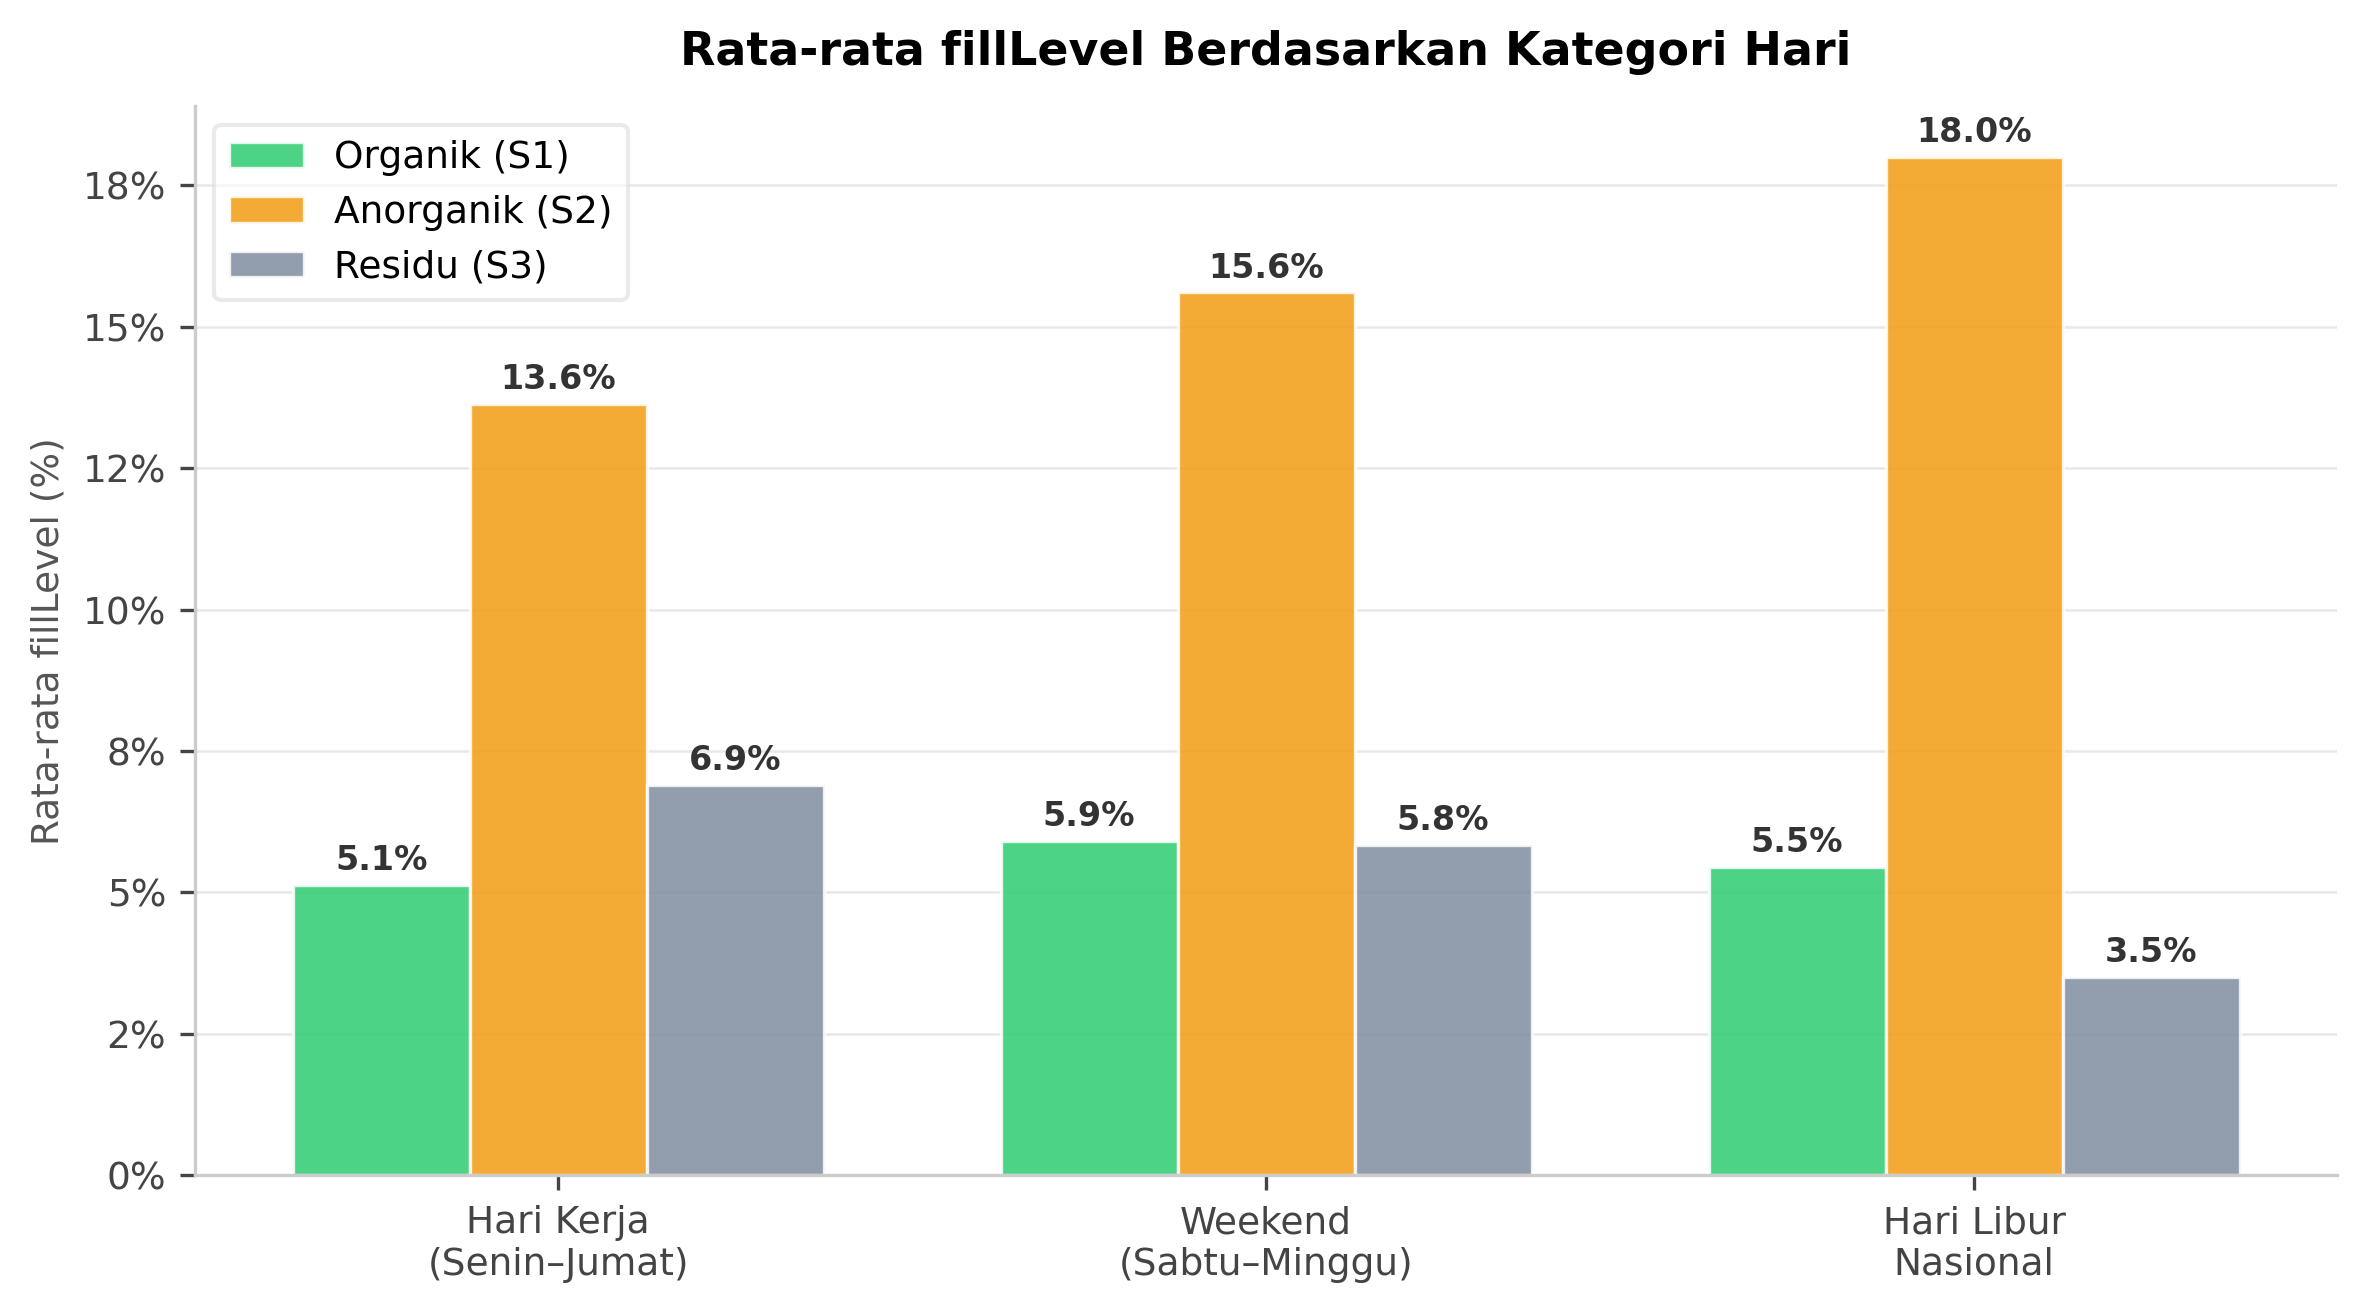
\includegraphics[width=0.8\textwidth]{images/pola-libur.png}
  % RENAME: image18.png → pola-libur.png
\end{figure}

Hari libur nasional yang memiliki data dalam periode pengumpulan meliputi 25 sampai 26 Desember 2025 (Natal) dan 1 Januari 2026 (Tahun Baru). Tingginya rata-rata \textit{fillLevel} Anorganik pada hari libur (18,0\%) merupakan efek akumulasi kumulatif, yaitu tempat sampah yang tidak dikosongkan saat libur membawa nilai \textit{fillLevel} dari hari-hari sebelumnya, bukan mencerminkan aktivitas pembuangan yang lebih tinggi.

\subsubsection{Analisis Penambahan (Delta)}

Analisis delta mengidentifikasi frekuensi dan waktu terjadinya penambahan sampah yang sesungguhnya. Tabel \ref{tab:analisis-delta} menyajikan proporsi jenis perubahan \textit{fillLevel}.

\begin{table}[H]
  \caption{Analisis Delta \textit{fillLevel}}
  \label{tab:analisis-delta}
  \centering
  \begin{tabular}{| l | l | l | l |}
    \hline
    \textbf{Jenis Perubahan} & \textbf{Organik} & \textbf{Anorganik} & \textbf{Residu} \\
    \hline
    Tidak ada perubahan ($\delta$ = 0)         & 95,5\% & 93,4\% & 94,2\% \\
    \hline
    Penambahan kecil (+10\%)                   & 2,4\%  & 3,8\%  & 3,1\% \\
    \hline
    Penambahan besar (+20\% atau lebih)        & 0\%    & 0,7\%  & 0\% \\
    \hline
    Pengurangan / dikosongkan ($\delta$ $<$ 0) & 2,1\%  & 2,1\%  & 2,7\% \\
    \hline
  \end{tabular}
\end{table}

Tabel \ref{tab:delta-perjam} menyajikan distribusi temporal \textit{event} penambahan berdasarkan rentang jam.

\begin{table}[H]
  \caption{Distribusi \textit{Event} Penambahan per Rentang Jam}
  \label{tab:delta-perjam}
  \centering
  \begin{tabular}{| l | l | l | l | l | l |}
    \hline
    \textbf{Rentang Jam} & \textbf{S1} & \textbf{S2} & \textbf{S3} & \textbf{Total} & \textbf{\% dari 27} \\
    \hline
    07:00--09:00 & 2 & 2 & 1 & 5  & 18,5\% \\
    \hline
    09:00--12:00 & 1 & 2 & 3 & 6  & 22,2\% \\
    \hline
    12:00--14:00 & 0 & 3 & 2 & 5  & 18,5\% \\
    \hline
    14:00--17:00 & 3 & 4 & 1 & 8  & 29,6\% \\
    \hline
    17:00--19:00 & 1 & 2 & 0 & 3  & 11,1\% \\
    \hline
    19:00--07:00 & 0 & 0 & 0 & 0  & 0\% \\
    \hline
    \textbf{Total} & \textbf{7} & \textbf{13} & \textbf{7} & \textbf{27} & \textbf{100\%} \\
    \hline
  \end{tabular}
\end{table}

\begin{figure}[H]
  \caption{Distribusi Kategori Delta dan \textit{Event} Penambahan per Rentang Jam}
  \label{fig:distribusi-delta}
  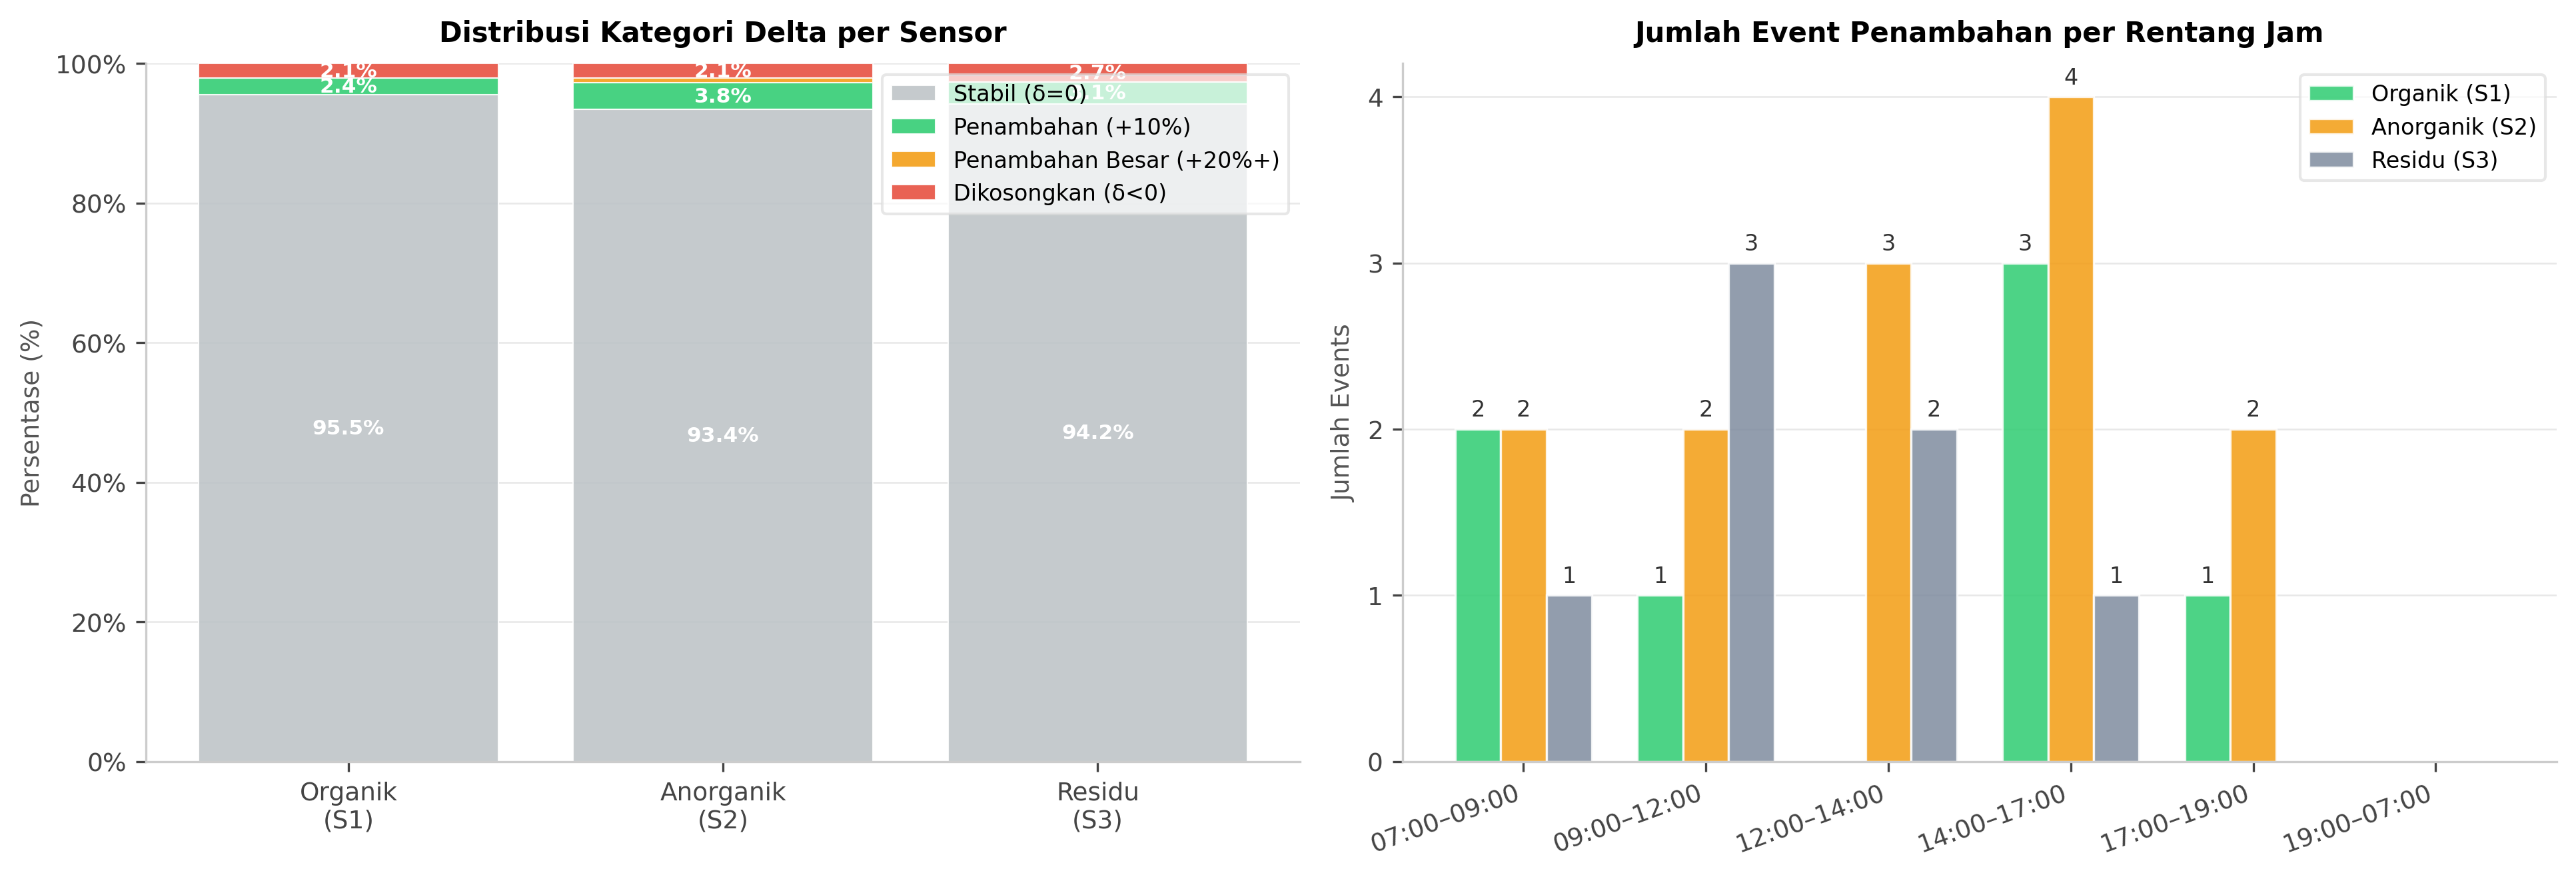
\includegraphics[width=\textwidth]{images/distribusi-delta.png}
  % RENAME: image19.png → distribusi-delta.png
\end{figure}

Total 27 \textit{event} penambahan terdeteksi selama periode observasi, dengan distribusi temporal divisualisasikan pada Gambar \ref{fig:distribusi-delta}. Penambahan terbanyak terjadi pada rentang 14:00--17:00 (29,6\%), diikuti 09:00--12:00 (22,2\%). Tidak ada penambahan yang terdeteksi pada malam hari (19:00--07:00), konsisten dengan tidak adanya aktivitas kampus.

\subsubsection{Analisis Komposisi Jenis Sampah}

Tabel \ref{tab:pola-jenis} menyajikan perbandingan pola pembuangan antar jenis sampah.

\begin{table}[H]
  \caption{Pola Setiap Jenis Sampah}
  \label{tab:pola-jenis}
  \begin{tabularx}{\textwidth}{| X | l | l | l |}
    \hline
    \textbf{Aspek} & \textbf{Organik (S1)} & \textbf{Anorganik (S2)} & \textbf{Residu (S3)} \\
    \hline
    Rata-rata \textit{fillLevel}          & 5,3\%    & 14,4\%    & 6,4\% \\
    \hline
    Max \textit{fillLevel} tercatat       & 20\%     & 40\%      & 20\% \\
    \hline
    Frekuensi penambahan                  & 2,4\%    & 4,5\%     & 3,1\% \\
    \hline
    Jumlah \textit{event} penambahan      & 7        & 13        & 7 \\
    \hline
    Total delta positif                   & +70\%    & +150\%    & +70\% \\
    \hline
    Korelasi dengan hari kerja            & Tinggi   & Sangat Tinggi & Tinggi \\
    \hline
  \end{tabularx}
\end{table}

\begin{figure}[H]
  \caption{Perbandingan Pola Jenis Sampah}
  \label{fig:perbandingan-jenis}
  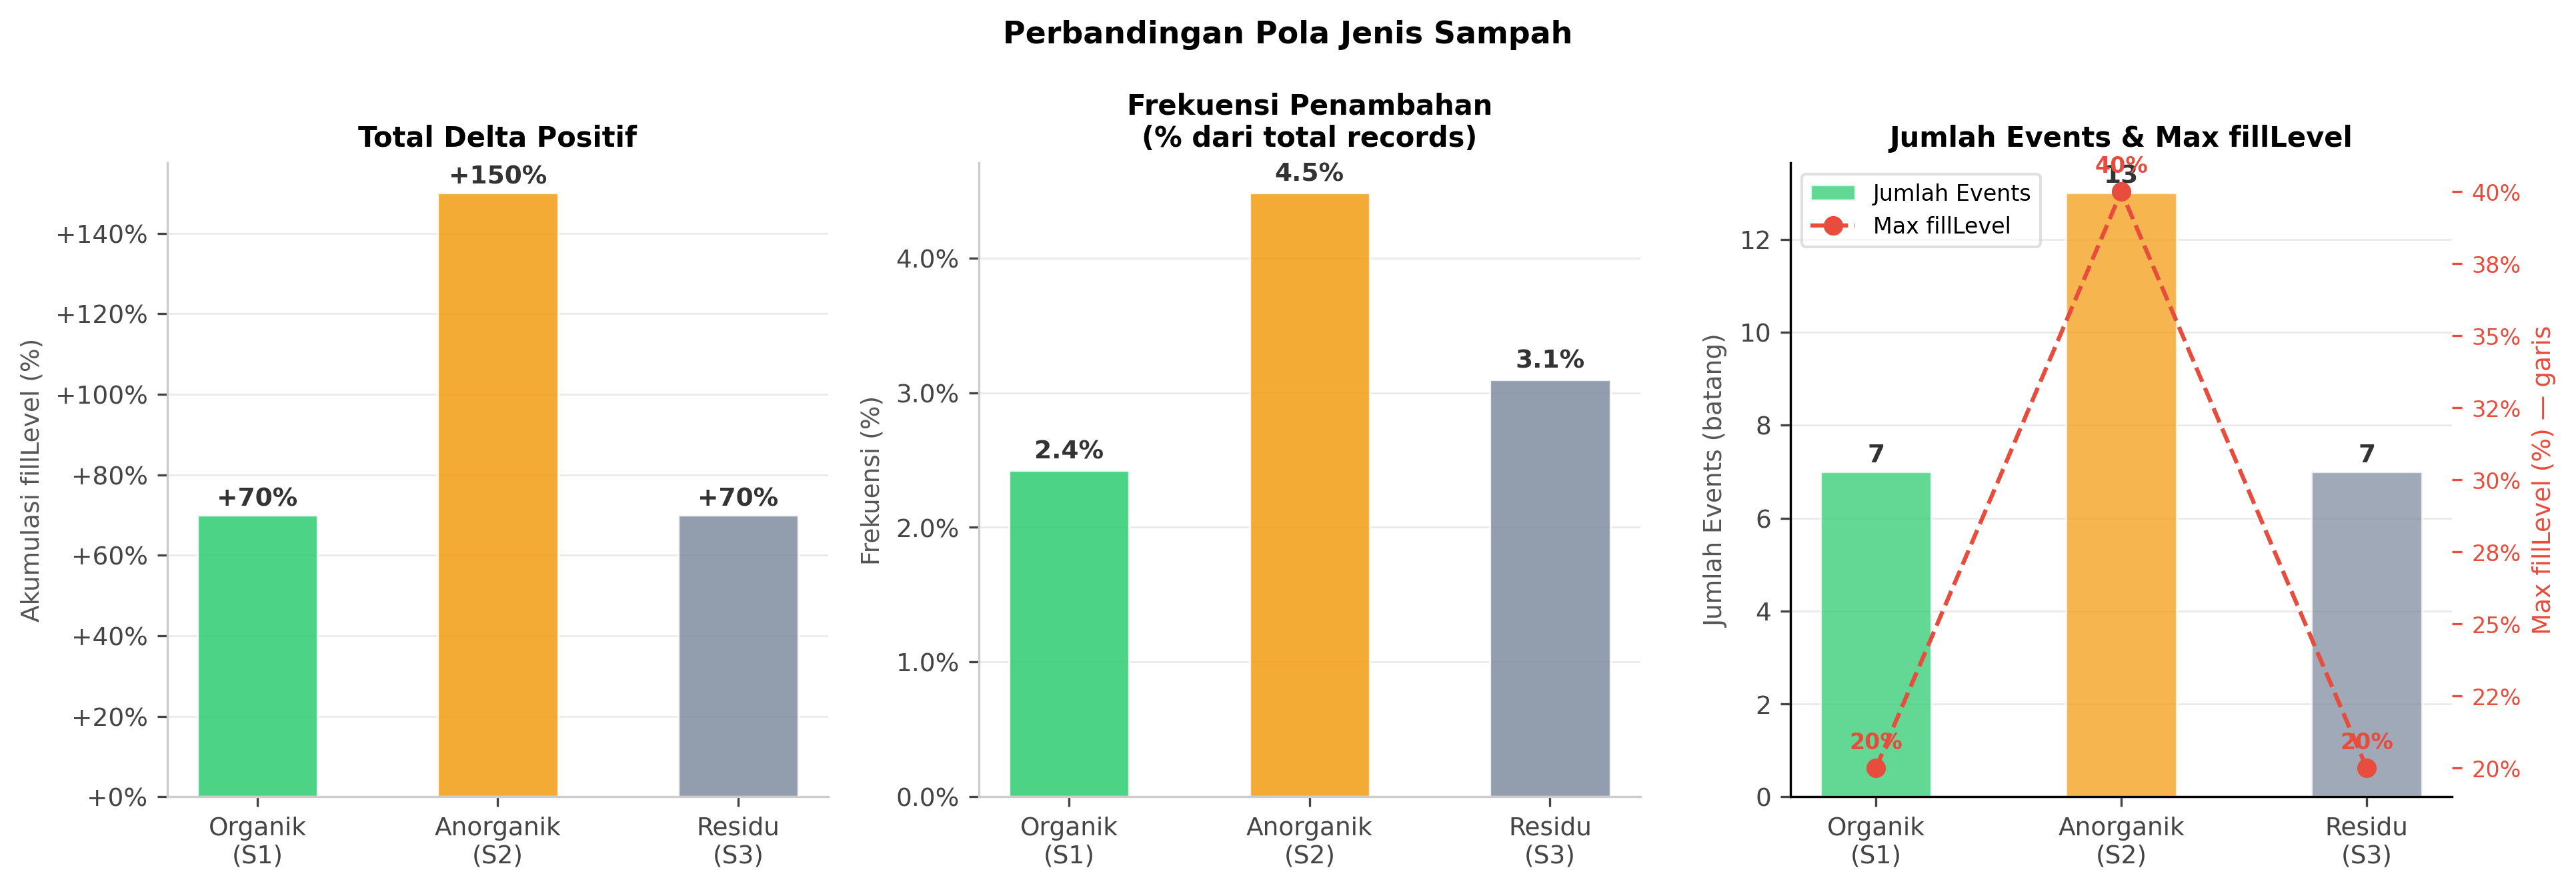
\includegraphics[width=\textwidth]{images/perbandingan-jenis.png}
  % RENAME: image20.png → perbandingan-jenis.png
\end{figure}

Sampah Anorganik memiliki volume dan frekuensi penambahan tertinggi (51,7\% dari total delta), sebagaimana divisualisasikan pada Gambar \ref{fig:perbandingan-jenis}. Organik dan Residu masing-masing berkontribusi 24,1\%. Hal ini sesuai dengan karakteristik lokasi sebagai area laboratorium yang menghasilkan lebih banyak sampah plastik, kertas, dan kemasan.

\subsubsection{Analisis Ketepatan Klasifikasi Sampah}

Selain analisis volume, dilakukan juga observasi terhadap ketepatan klasifikasi sampah oleh pengguna. Observasi visual dilakukan pada beberapa waktu \textit{sampling} untuk mengidentifikasi sampah yang dibuang pada kategori yang tidak sesuai peruntukannya (lihat Lampiran C). Berdasarkan dokumentasi foto yang tersedia, temuan observasi ketepatan klasifikasi disajikan pada Tabel \ref{tab:kesesuaian-jenis}.

\begin{table}[H]
  \caption{Kesesuaian Jenis Sampah}
  \label{tab:kesesuaian-jenis}
  \begin{tabularx}{\textwidth}{| l | X | l |}
    \hline
    \textbf{Tempat Sampah} & \textbf{Temuan} & \textbf{Validasi Lapangan} \\
    \hline
    Organik (Hijau) & Ditemukan kantong plastik dan sisa bungkus makanan & Terdokumentasi foto (Lampiran C) \\
    \hline
    Anorganik (Kuning) & Ditemukan beberapa sisa tisu basah yang seharusnya masuk ke residu & Terdokumentasi foto (Lampiran C) \\
    \hline
    Residu (Hitam) & Ditemukan sisa makanan dalam wadah dan tisu bekas & Terdokumentasi foto (Lampiran C) \\
    \hline
  \end{tabularx}
\end{table}

Temuan utama dari observasi ketepatan klasifikasi adalah sebagai berikut.

\begin{enumerate}
  \item \textbf{Plastik di Tempat Sampah Organik.} Ditemukan plastik kemasan makanan di tempat sampah organik. Pengguna cenderung membuang kemasan makanan beserta sisa makanannya sekaligus karena dianggap satu kesatuan.

  \item \textbf{Residu di Tempat Sampah Anorganik.} Ditemukan sampah yang seharusnya masuk kategori residu seperti tisu kotor dan \textit{styrofoam} di tempat sampah anorganik, kemungkinan karena kurangnya pemahaman tentang definisi sampah residu.

  \item \textbf{Campuran di Tempat Sampah Residu.} Tempat sampah residu ditemukan mengandung sisa makanan yang seharusnya masuk kategori organik. Hal ini mengindikasikan bahwa pengguna mengalami kebingungan dalam mengidentifikasi kategori residu, yang memang memiliki definisi paling tidak intuitif dibandingkan kategori organik dan anorganik.
\end{enumerate}

Temuan ini menunjukkan perlunya sosialisasi berkala tentang jenis sampah dan penyediaan infografis panduan singkat di dekat lokasi tempat sampah untuk meningkatkan ketepatan klasifikasi oleh pengguna.

\subsubsection{Sintesis Temuan Analisis}
\label{sec:sintesis-temuan}

Seluruh analisis pada subbab ini dilakukan menggunakan pendekatan \textit{analisis deskriptif}, yaitu pendekatan yang bertujuan mendeskripsikan dan merangkum karakteristik suatu fenomena berdasarkan data, tanpa melakukan inferensi kausal maupun prediksi \autocite{loeb2017descriptive}. Pendekatan ini dipilih karena tujuan penelitian adalah mengidentifikasi dan mengkarakterisasi pola pembuangan yang terjadi, bukan memodelkan atau memprediksinya. Analisis deskriptif terhadap data deret waktu (\textit{time series}) yang dikumpulkan mencakup peringkasan statistik, agregasi temporal, dan visualisasi untuk mengungkap struktur dalam data \autocite{wickham2016r}.

Berdasarkan analisis deskriptif yang dilakukan, penelitian ini mengidentifikasi empat pola pembuangan sampah. Sebuah pola didefinisikan sebagai keteraturan yang konsisten muncul dalam data sepanjang periode pengamatan, bukan kejadian tunggal yang bersifat acak. Keempat pola ini dibedakan menjadi dua jenis berdasarkan dimensi analisisnya, yaitu tiga \textbf{pola temporal} (keteraturan pada dimensi waktu) dan satu \textbf{pola komposisi} (keteraturan pada dimensi jenis sampah). Setiap pola diberi nama yang jelas sebagai identitasnya. Tabel \ref{tab:sintesis-temuan} merangkum keempat pola tersebut beserta klasifikasinya.

\begin{table}[H]
  \caption{Sintesis dan Klasifikasi Pola Pembuangan Sampah}
  \label{tab:sintesis-temuan}
  \begin{tabularx}{\textwidth}{| l | l | X |}
    \hline
    \textbf{Nama Pola} & \textbf{Jenis} & \textbf{Deskripsi Kuantitatif} \\
    \hline
    Pola \textit{Peak Hour} & Pola Temporal & Puncak penambahan pada pukul 14:00--17:00 (8 dari 27 \textit{event}, 29,6\%) \\
    \hline
    Pola Konsentrasi Jam Aktif & Pola Temporal & Seluruh \textit{event} terjadi pada rentang 07:00--19:00 di hari kerja \\
    \hline
    Pola Pengaruh Hari Libur & Pola Temporal & Aktivitas penambahan turun hingga nol pada hari libur nasional \\
    \hline
    Pola Dominasi Anorganik & Pola Komposisi & Sampah anorganik menyumbang 13 dari 27 \textit{event} (48,1\%) dan 51,7\% volume delta positif \\
    \hline
  \end{tabularx}
\end{table}

Ketiga pola temporal, yaitu Pola \textit{Peak Hour}, Pola Konsentrasi Jam Aktif, dan Pola Pengaruh Hari Libur, merupakan keteraturan yang muncul pada dimensi waktu dan saling melengkapi dalam menggambarkan kapan aktivitas pembuangan terjadi. Sementara itu, Pola Dominasi Anorganik merupakan keteraturan pada dimensi komposisi jenis sampah, yang konsisten muncul sepanjang periode pengamatan (bukan fluktuasi acak), sehingga sah dikategorikan sebagai pola meskipun tidak berdimensi waktu. Keempat pola ini telah divalidasi kewajarannya terhadap observasi lapangan dan konsisten dengan karakteristik aktivitas di lokasi penelitian, serta secara bersama-sama menjawab RM-2.

\subsection{Hasil Evaluasi Adaptasi \textit{Firmware} (SE-04)}

Skenario SE-04 mengevaluasi efektivitas adaptasi \textit{firmware} yang dilakukan terhadap perangkat \textit{Smart Waste Bin}. Evaluasi ini merupakan bagian dari penilaian keberhasilan rancangan dan implementasi sistem (RM-1), khususnya untuk menilai sejauh mana adaptasi \textit{firmware} meningkatkan keandalan operasional dan kualitas data yang dikumpulkan sistem.

Tabel \ref{tab:hasil-firmware} menyajikan hasil evaluasi untuk setiap adaptasi \textit{firmware}.

\begin{table}[H]
  \caption{Hasil Evaluasi Adaptasi \textit{Firmware}}
  \label{tab:hasil-firmware}
  \begin{tabularx}{\textwidth}{| X | X | X | l |}
    \hline
    \textbf{Peningkatan} & \textbf{Masalah yang Diatasi} & \textbf{Hasil Evaluasi} & \textbf{Status} \\
    \hline
    Perubahan interval (8 jam → 2,5 jam) & Resolusi data terlalu rendah untuk analisis pola temporal & 8--9 data \textit{points} per hari, pola harian berhasil teridentifikasi & Efektif \\
    \hline
    \textit{Median filter} (5 \textit{readings}) & \textit{Noise} pada pembacaan sensor & \textit{fillLevel} stabil tanpa lompatan acak & Efektif \\
    \hline
    \textit{Auto-recovery mechanism} & Sensor \textit{hang} menyebabkan \textit{data loss} & Tidak ada kejadian \textit{hang} setelah implementasi & Efektif \\
    \hline
    \textit{Warm-up readings} & Pembacaan awal tidak stabil & Pembacaan pertama lebih konsisten & Efektif \\
    \hline
    GPIO \textit{isolation} & \textit{Floating state} saat \textit{sleep} & Konsumsi daya tidak berubah signifikan & Tidak Efektif \\
    \hline
  \end{tabularx}
\end{table}

Dari lima adaptasi \textit{firmware} yang diimplementasikan, empat menunjukkan efektivitas. Perubahan interval pengambilan data menjadi fondasi keberhasilan analisis pola. \textit{Median filter} berhasil mereduksi \textit{noise} selama periode pengujian. Mekanisme \textit{auto-recovery} terbukti efektif karena sebelum implementasi, sensor pernah mengalami kondisi \textit{hang} dan tidak mengirim data meskipun baterai masih baik, namun setelah \textit{firmware} baru di-\textit{upload}, kejadian tersebut tidak terulang. Satu adaptasi yang tidak efektif adalah GPIO \textit{isolation}, kemungkinan karena konsumsi daya utama berasal dari modul GSM SIM800L yang tidak terpengaruh oleh isolasi GPIO.

% ============================================================
\section{Pemenuhan Kebutuhan Sistem}
\label{sec:pemenuhan-kebutuhan}
% ============================================================

Subbab ini menyajikan evaluasi pemenuhan kebutuhan fungsional dan nonfungsional yang telah diidentifikasi pada Bab III, berdasarkan hasil pengujian pada Subbab \ref{sec:hasil-evaluasi}.

\subsection{Pemenuhan Kebutuhan Fungsional}

Tabel \ref{tab:pemenuhan-kf-hasil} menyajikan evaluasi pemenuhan seluruh kebutuhan fungsional.

\begin{table}[H]
  \caption{Pemenuhan Kebutuhan Fungsional}
  \label{tab:pemenuhan-kf-hasil}
  \begin{tabularx}{\textwidth}{| l | X | X | l |}
    \hline
    \textbf{ID} & \textbf{Kebutuhan Fungsional} & \textbf{Bukti Pemenuhan} & \textbf{Status} \\
    \hline
    KF-01 & Pembacaan tingkat kepenuhan & Sensor VL53L0X membaca jarak dan mengkonversi ke \textit{fillLevel} & Terpenuhi \\
    \hline
    KF-02 & Transmisi data otomatis periodik & Data terkirim setiap $\sim$2,5 jam via MQTT & Terpenuhi \\
    \hline
    KF-03 & \textit{Timestamp} dan \textit{identifier} & Setiap \textit{record} memiliki \textit{timestamp} dan \texttt{sensor\_id} & Terpenuhi \\
    \hline
    KF-04 & Konversi jarak ke persentase & \textit{Firmware} mengkonversi mm ke \% menggunakan rumus konversi & Terpenuhi \\
    \hline
    KF-05 & Penyimpanan data ke \textit{database} & Data tersimpan di Supabase PostgreSQL & Terpenuhi \\
    \hline
    KF-06 & \textit{Query} data berdasarkan \textit{filter} & API mendukung \textit{filter} \texttt{sensorId} dan \texttt{timerange} & Terpenuhi \\
    \hline
    KF-07 & Analisis pola temporal & Pola harian, mingguan, dan libur teridentifikasi & Terpenuhi \\
    \hline
    KF-08 & Statistik deskriptif & \textit{Mean}, median, std dev dihitung per sensor & Terpenuhi \\
    \hline
    KF-09 & Visualisasi data \textit{dashboard} & \textit{Dashboard} menampilkan \textit{chart} dan status terkini & Terpenuhi \\
    \hline
    KF-10 & Grafik pola temporal & \textit{Line chart} menampilkan tren \textit{fillLevel} & Terpenuhi \\
    \hline
  \end{tabularx}
\end{table}

Seluruh kebutuhan fungsional (KF-01 sampai KF-10) berhasil dipenuhi oleh sistem yang diimplementasikan.

\subsection{Pemenuhan Kebutuhan Nonfungsional}

Tabel \ref{tab:pemenuhan-knf-hasil} menyajikan evaluasi pemenuhan kebutuhan nonfungsional.

\begin{table}[H]
  \caption{Pemenuhan Kebutuhan Nonfungsional}
  \label{tab:pemenuhan-knf-hasil}
  \begin{tabularx}{\textwidth}{| l | X | l | l | l | l |}
    \hline
    \textbf{ID} & \textbf{Kebutuhan} & \textbf{Target} & \textbf{Aktual} & \textbf{Kategori} & \textbf{Status} \\
    \hline
    KNF-01 & Waktu pembacaan sensor       & $<$ 1 menit & $<$ 5 detik & \textit{Performance} & Terpenuhi \\
    \hline
    KNF-02 & Latensi transmisi data       & $<$ 10 detik & $<$ 3 detik & \textit{Performance} & Terpenuhi \\
    \hline
    KNF-03 & \textit{Response time dashboard} & $<$ 3 detik & $<$ 1 detik & \textit{Performance} & Terpenuhi \\
    \hline
    KNF-04 & Waktu \textit{query database} & $<$ 5 detik & $<$ 500 ms & \textit{Performance} & Terpenuhi \\
    \hline
    KNF-05 & \textit{Uptime} sistem IoT   & $>$ 95\% & 91,9\% & \textit{Reliability} & Sebagian \\
    \hline
    KNF-06 & Konsistensi interval         & $\pm$15 menit & $\pm$12 menit* & \textit{Reliability} & Terpenuhi \\
    \hline
    KNF-07 & Kelengkapan data             & $>$ 90\% & 91,9\% & \textit{Reliability} & Terpenuhi \\
    \hline
    KNF-08 & Akurasi sensor \textit{fillLevel} & $<$ 10\% \textit{error} & Sesuai & \textit{Accuracy} & Terpenuhi \\
    \hline
  \end{tabularx}
\end{table}

*KNF-06 dihitung berdasarkan Sensor 1 dan 2. Sensor 3 memiliki std dev 38 menit yang melebihi toleransi akibat anomali konsumsi daya.

KNF-05 dan KNF-07 menggunakan metrik yang sama (91,9\%) namun berstatus berbeda karena \textit{threshold} yang berbeda. KNF-05 menargetkan 95\% sehingga berstatus sebagian, sedangkan KNF-07 menargetkan 90\% sehingga terpenuhi. Dari 8 kebutuhan nonfungsional, 7 berhasil dipenuhi sepenuhnya dan 1 kebutuhan (KNF-05) dipenuhi sebagian karena faktor eksternal berupa \textit{broker} MQTT vendor yang dimatikan dan baterai bocor.

% ============================================================
\section{Diskusi Hasil Evaluasi}
\label{sec:diskusi-evaluasi}
% ============================================================

\subsection{Analisis Konsumsi Daya pada Sensor 3}

Sensor 3 (Residu) menunjukkan anomali berupa konsumsi arus hampir dua kali lipat (210--235 mA) dibandingkan Sensor 1 dan 2 (110--140 mA), meskipun ketiga unit menggunakan spesifikasi komponen identik dan \textit{firmware} yang sama. Anomali ini menyebabkan baterai Sensor 3 lebih cepat habis dan mengakibatkan \textit{data loss} lebih tinggi (23,6\%) dibandingkan sensor lainnya ($\sim$2\%).

Berbagai upaya optimasi \textit{firmware} telah dilakukan termasuk GPIO \textit{isolation} dan optimasi urutan \textit{shutdown}, namun konsumsi daya tetap tinggi. Ini mengindikasikan akar masalah bukan pada \textit{software} melainkan \textit{hardware}. Beberapa hipotesis penyebab: komponen pasif yang rusak atau tidak terpasang dengan benar, \textit{short circuit} ringan pada PCB, variasi karakteristik komponen aktif seperti modul SIM800L, atau kerusakan pada jalur \textit{power} akibat proses \textit{assembly}.

Temuan ini menunjukkan pentingnya \textit{quality control} dan \textit{burn-in testing} sebelum \textit{deployment} perangkat IoT. Untuk produksi massal, disarankan menetapkan batas toleransi konsumsi daya dan melakukan \textit{reject} pada unit yang melebihi batas tersebut.

\subsection{Validitas Temuan}

Untuk memastikan validitas pola yang teridentifikasi, dilakukan triangulasi dengan observasi kontekstual lapangan berdasarkan pengetahuan kondisi aktual lokasi penelitian dan dokumentasi foto (Lampiran C). Tabel \ref{tab:validasi-pola} menyajikan validasi setiap pola terhadap kondisi aktual di lapangan.

\begin{table}[H]
  \caption{Validasi Pola dengan Observasi Lapangan}
  \label{tab:validasi-pola}
  \begin{tabularx}{\textwidth}{| l | X | X | X |}
    \hline
    \textbf{No} & \textbf{Pola Teridentifikasi} & \textbf{Evidensi Data} & \textbf{Validasi Lapangan} \\
    \hline
    1 & \textit{Peak hour} pada pukul 14:00--17:00 & 8 \textit{event} penambahan terdeteksi pada rentang ini, tertinggi dari semua rentang (29,6\% dari 27 \textit{event}) & Konsisten dengan jadwal aktivitas lab; warga lab umumnya membuang sampah setelah sesi kerja siang \\
    \hline
    2 & Aktivitas pembuangan pada hari kerja lebih tinggi & Seluruh 27 \textit{event} penambahan terjadi pada jam aktif kampus 07:00--19:00, tidak ada penambahan pada malam hari dan \textit{weekend} & Dikonfirmasi; Lab IoT tidak beroperasi di luar jam kerja dan akses terbatas \\
    \hline
    3 & Aktivitas pembuangan turun drastis pada hari libur nasional & Tidak ada \textit{event} penambahan terdeteksi pada hari libur; \textit{fillLevel} Anorganik tinggi (18,0\%) merupakan efek akumulasi kumulatif & Dikonfirmasi; gedung tidak beroperasi pada 25--26 Des dan 1 Jan \\
    \hline
    4 & Dominasi sampah anorganik (51,7\% dari total volume) & Anorganik menyumbang +150\% delta positif dari total +290\%, setara 51,7\% dari total \textit{event} penambahan (13 dari 27) & Konsisten dengan observasi; pengguna lab menghasilkan kemasan minuman dan makanan lebih banyak \\
    \hline
  \end{tabularx}
\end{table}

Seluruh pola utama tervalidasi melalui observasi lapangan, meningkatkan \textit{confidence} bahwa pola-pola yang teridentifikasi mencerminkan kondisi aktual, bukan artefak dari keterbatasan sensor atau \textit{noise} data.

\subsection{Implikasi Praktis Pengelolaan Sampah}

Temuan penelitian ini memiliki beberapa implikasi praktis untuk pengelolaan sampah di lingkungan kampus.

\begin{enumerate}
  \item Berdasarkan pola \textit{peak hour}, jadwal pengosongan tempat sampah dapat difokuskan pada sore hari kerja (setelah pukul 14:00), bukan pagi hari atau \textit{weekend}, untuk efisiensi operasional.

  \item Dominasi sampah anorganik (51,7\%) menunjukkan potensi program pengurangan kemasan sekali pakai atau penyediaan fasilitas \textit{refill} untuk menekan volume sampah.

  \item Empat dari lima adaptasi \textit{firmware} yang telah diuji dapat direkomendasikan untuk diadopsi pada perangkat \textit{Smart Waste Bin} di lingkungan dengan aktivitas terkonsentrasi pada jam-jam tertentu.

  \item Sistem Pemantauan Sampah Berbasis \textit{Internet of Things} memberikan data objektif untuk pengambilan keputusan pengelolaan sampah, menggantikan estimasi manual yang subjektif dan tidak terstruktur.
\end{enumerate}
\cleardoublepage
\chapter{KESIMPULAN DAN SARAN}
\label{chap:penutup}

Bab ini merangkum temuan-temuan utama dari hasil perancangan, implementasi, dan pengujian sistem \textit{Smart Waste Bin}, serta menguraikan rekomendasi praktis dan akademis untuk pengembangan penelitian maupun penyempurnaan perangkat di masa mendatang.

% ============================================================
\section{Kesimpulan}
\label{sec:kesimpulan}
% ============================================================

Penelitian ini telah berhasil mengembangkan dan mengimplementasikan sistem \textit{Smart Waste Bin} berbasis \textit{Internet of Things} (IoT) untuk keperluan otomatisasi pengumpulan data dan analisis pola pembuangan sampah di Gedung Labtek VIII Institut Teknologi Bandung, khususnya pada Laboratorium \textit{Internet of Things} Lantai 4. Selama periode observasi 37 hari, sistem berhasil mengumpulkan 816 \textit{records} data dari tiga unit perangkat sensor dengan tingkat keberhasilan pengiriman mencapai 91,9\%, dengan 805 \textit{records} valid setelah \textit{filtering} data kotor. Berdasarkan hasil evaluasi menyeluruh pada Bab VI, seluruh rumusan masalah dalam penelitian ini telah berhasil dijawab dengan rincian sebagai berikut.

\begin{enumerate}
  \item \textbf{Rancangan dan Implementasi Sistem (Menjawab RM-1)}

  Penelitian ini berhasil merancang sistem \textit{Smart Waste Bin} terintegrasi dengan arsitektur IoT 4-\textit{layer}. Arsitektur ini mencakup \textit{Perception Layer} (ESP32, VL53L0X, INA219, SIM800L) untuk akuisisi data fisik, \textit{Network Layer} (MQTT) untuk transmisi nirkabel, \textit{Middleware Layer} (Node-RED) untuk pemrosesan aliran data, dan \textit{Application Layer} (Supabase, Next.js) untuk penyimpanan dan visualisasi antarmuka. Seluruh komponen terbukti berfungsi sesuai dengan desain, di mana 10 kebutuhan fungsional dan 7 dari 8 kebutuhan nonfungsional telah terpenuhi.

  \item \textbf{Identifikasi Pola Pembuangan Sampah (Menjawab RM-2)}

  Melalui analisis data historis dan analisis delta, sistem berhasil mengidentifikasi empat pola temporal pembuangan sampah di lingkungan kampus yang telah divalidasi melalui observasi lapangan, yaitu:

  \begin{enumerate}[a.]
    \item \textit{Peak hour} (jam sibuk) secara konsisten pada pukul 14:00 sampai 17:00, ditunjukkan oleh 8 \textit{event} penambahan (29,6\% dari total 27 \textit{event}). Pola ini konsisten dengan perilaku membuang sampah setelah aktivitas makan siang.

    \item Seluruh \textit{event} penambahan sampah terjadi pada jam aktif hari kerja (07:00 sampai 19:00), tanpa satu pun penambahan yang terdeteksi pada malam hari maupun akhir pekan.

    \item Aktivitas pembuangan sampah turun drastis pada hari libur nasional, di mana tidak terdeteksi adanya \textit{event} penambahan pada 25 sampai 26 Desember 2025 dan 1 Januari 2026. Nilai \textit{fillLevel} tinggi pada hari libur merupakan efek akumulasi kumulatif, bukan cerminan aktivitas pembuangan.

    \item Dominasi sampah anorganik yang menyumbang 13 dari 27 \textit{event} penambahan (48,1\%) dengan total delta positif sebesar 150\%, konsisten dengan karakteristik lokasi sebagai area laboratorium yang menghasilkan banyak sampah kemasan sekali pakai.
  \end{enumerate}

  \item \textbf{Peningkatan \textit{Firmware Smart Waste Bin} (Menjawab RM-3)}

  Perangkat bawaan dari pihak ketiga telah berhasil dioptimasi melalui lima peningkatan \textit{firmware} agar sesuai dengan kebutuhan lingkungan kampus, meliputi perubahan interval pengambilan data, implementasi \textit{median filter}, mekanisme \textit{auto-recovery}, \textit{warm-up readings}, dan GPIO \textit{isolation}. Empat dari lima peningkatan terbukti efektif dalam mengatasi masalah yang ditargetkan. GPIO \textit{isolation} tidak menunjukkan perubahan signifikan pada konsumsi daya karena sumber konsumsi utama berasal dari modul GSM yang tidak terpengaruh oleh kondisi GPIO. Peningkatan yang terbukti efektif dapat direkomendasikan untuk diadopsi pada produk \textit{Smart Waste Bin} standar vendor, khususnya untuk \textit{deployment} di lingkungan dengan karakteristik aktivitas yang terkonsentrasi pada jam-jam tertentu.
\end{enumerate}

% ============================================================
\section{Saran}
\label{sec:saran}
% ============================================================

Penelitian ini masih memiliki sejumlah keterbatasan yang membuka peluang untuk pengembangan lebih lanjut. Berdasarkan temuan dan kendala yang dihadapi selama pelaksanaan penelitian, saran dibagi menjadi dua kelompok, yaitu saran untuk penelitian selanjutnya dan saran untuk penyedia teknologi \textit{Smart Waste Bin}.

\subsection{Saran untuk Penelitian Selanjutnya}

Bagi peneliti yang ingin mengembangkan penelitian serupa, terdapat beberapa aspek yang dapat ditingkatkan sebagai berikut.

\begin{enumerate}
  \item Penggunaan tempat sampah berukuran lebih kecil disarankan agar resolusi pengukuran \textit{fillLevel} menjadi lebih tinggi. Pada penelitian ini, pengukuran terbatas pada kelipatan 10\% akibat penggunaan tipe data integer pada \textit{firmware}.

  \item Periode pengumpulan data perlu diperpanjang minimal satu semester untuk memperoleh pola yang lebih representatif. Periode yang lebih panjang juga memungkinkan validasi pola mingguan dengan tingkat keyakinan yang lebih tinggi.

  \item Penambahan sensor pada beberapa titik (\textit{multi-point}) dapat dipertimbangkan untuk mendeteksi sampah yang menumpuk di pinggir tempat sampah. Kondisi ini tidak terdeteksi pada penelitian ini karena menggunakan konfigurasi sensor \textit{single-point}.

  \item Program sosialisasi pemilahan sampah dapat dikombinasikan dengan penerapan sistem untuk menekan tingkat kesalahan klasifikasi sampah, sebagaimana ditemukan pada observasi lapangan dalam penelitian ini.
\end{enumerate}

\subsection{Saran untuk Penyedia Teknologi \textit{Smart Waste Bin}}

Bagi penyedia perangkat \textit{Smart Waste Bin}, beberapa rekomendasi berikut dapat dipertimbangkan untuk meningkatkan kualitas produk.

\begin{enumerate}
  \item Ditemukan variasi konsumsi arus hampir dua kali lipat antar unit dengan spesifikasi identik, yaitu 110 sampai 140 mA pada dua unit dan 210 sampai 235 mA pada satu unit. Investigasi terhadap kebocoran daya pada jalur komponen perlu dilakukan, termasuk penerapan \textit{quality control} dan \textit{burn-in testing} sebelum perangkat dipasarkan.

  \item Empat peningkatan \textit{firmware} yang terbukti efektif, yaitu perubahan interval, \textit{median filter}, \textit{auto-recovery}, dan \textit{warm-up readings}, dapat diadopsi ke produk standar untuk meningkatkan keandalan sistem, khususnya di lingkungan dengan karakteristik aktivitas yang dinamis.

  \item Dokumentasi teknis perlu dilengkapi dengan skema rangkaian dan \textit{source code firmware} agar mempermudah proses pemeliharaan dan \textit{troubleshooting} oleh pengguna.
\end{enumerate}

% ==========================================
% DAFTAR PUSTAKA
% ==========================================
\clearpage
\printbibliography[title={DAFTAR PUSTAKA}]

% ==========================================
% LAMPIRAN
% ==========================================
\appendix
\begin{appendices}
\chapter{TAUTAN PENTING}
\label{chap:lampiran-a}

Tabel \ref{tab:tautan-penting} menyajikan tautan repositori dan \textit{deployment} yang berkaitan dengan penelitian ini.

\begin{table}[H]
  \caption{Tautan Penting}
  \label{tab:tautan-penting}
  \begin{tabularx}{\textwidth}{| l | X | X |}
    \hline
    \textbf{No} & \textbf{Tautan} & \textbf{Deskripsi} \\
    \hline
    1 & \url{https://github.com/Mipol2/TA-Node-RED} & Repositori Node-RED \\
    \hline
    2 & \url{https://github.com/Mipol2/TA-Firmware-ESP32} & Repositori \textit{Firmware} ESP32 \\
    \hline
    3 & \url{https://github.com/Mipol2/TA-Dasboard} & Repositori \textit{Dashboard} \\
    \hline
    4 & \url{https://github.com/Mipol2/TA-Data-Cleaner-Visual} & Repositori \textit{Dataset} Pengukuran Sampah serta \textit{Data Cleaner} dan \textit{Data Visualization} \\
    \hline
    5 & \url{https://dashboard-ta-mef7.vercel.app/} & \textit{Smart Waste Bin} IoT \textit{Dashboard} yang telah di-\textit{deploy} \\
    \hline
  \end{tabularx}
\end{table}
\chapter{ANTARMUKA \textit{DASHBOARD}}
\label{chap:lampiran-b}

Lampiran ini menyajikan tampilan lengkap antarmuka \textit{dashboard Smart Waste Bin}
yang telah diimplementasikan dan di-\textit{deploy} pada \textit{platform} Vercel.

\begin{figure}[H]
  \caption{Tampilan Keseluruhan \textit{Dashboard Smart Waste Bin}}
  \label{fig:lamp-dashboard-full}
  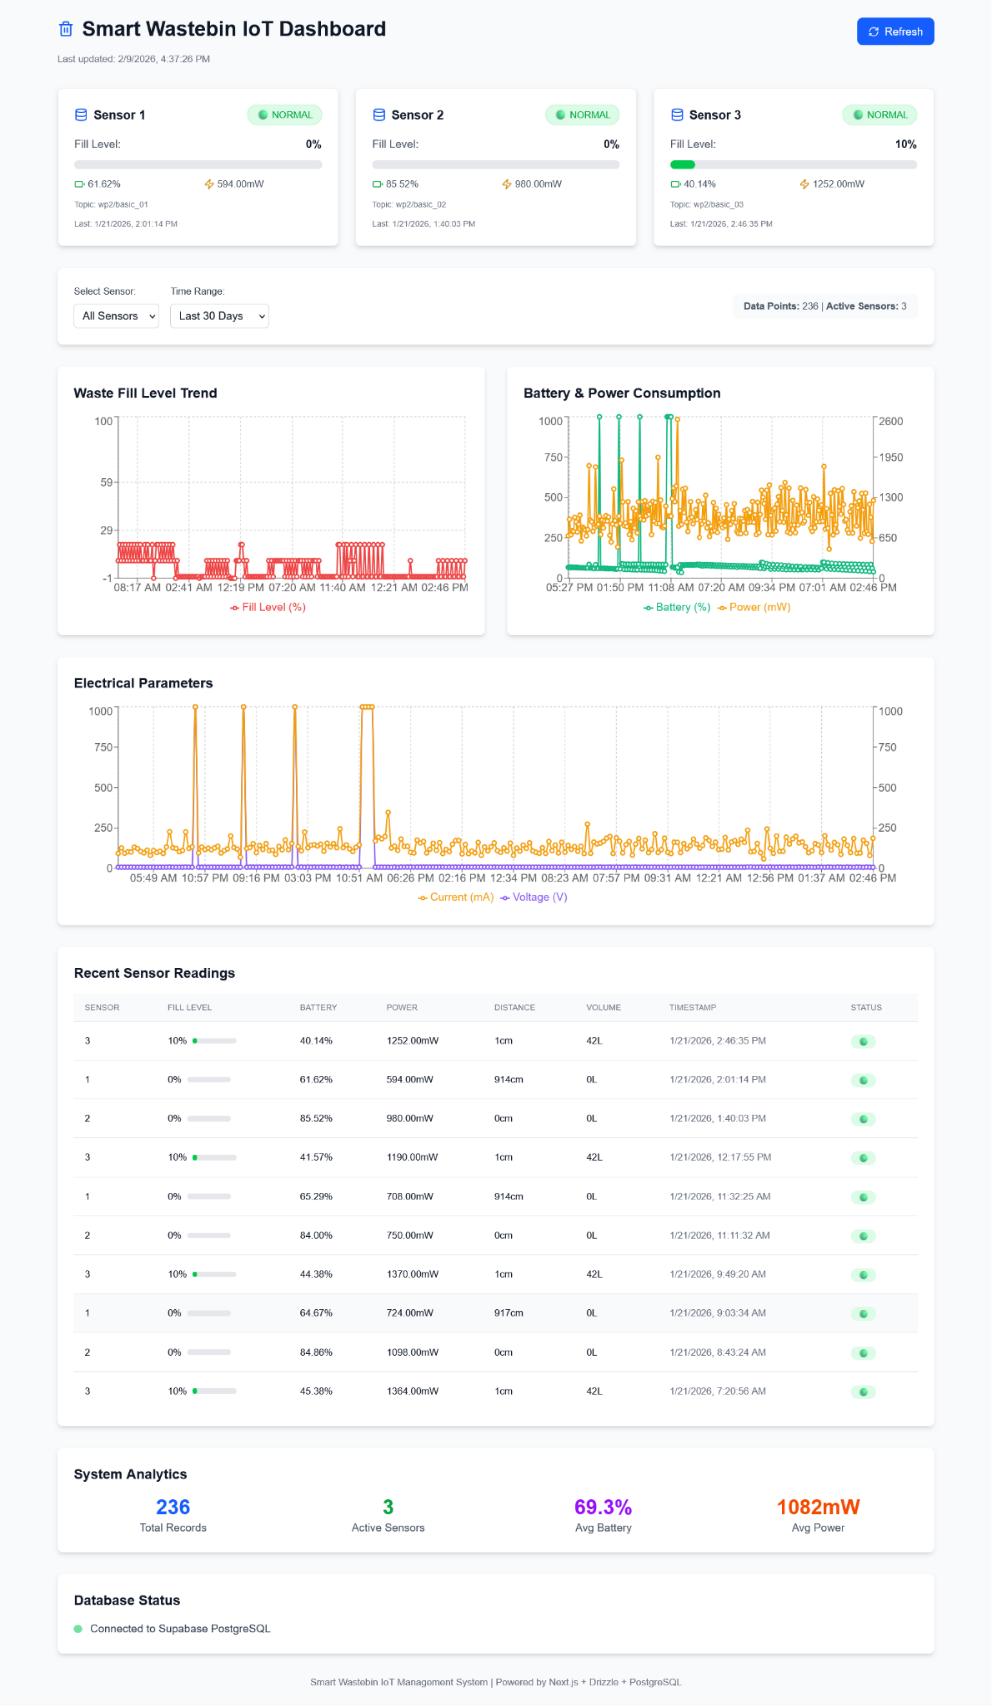
\includegraphics[width=0.85\textwidth]{images/dashboard-full.png}
  % RENAME: image21.png → dashboard-full.png
\end{figure}

\begin{figure}[H]
  \caption{\textit{Header Section Dashboard}}
  \label{fig:lamp-header}
  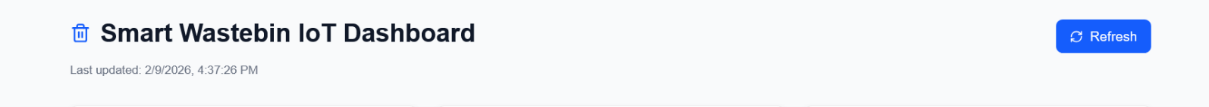
\includegraphics[width=\textwidth]{images/dashboard-header.png}
  % RENAME: image22.png → dashboard-header.png
\end{figure}

\begin{figure}[H]
  \caption{\textit{Sensor Status Cards}}
  \label{fig:lamp-cards}
  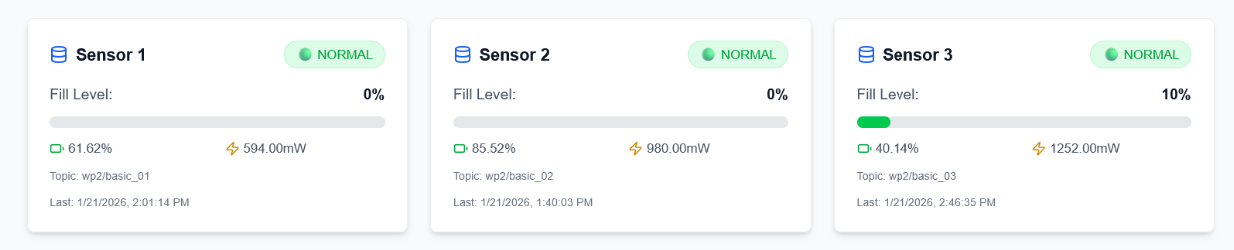
\includegraphics[width=\textwidth]{images/dashboard-cards.png}
  % RENAME: image23.png → dashboard-cards.png
\end{figure}

\begin{figure}[H]
  \caption{\textit{Control Panel}}
  \label{fig:lamp-control}
  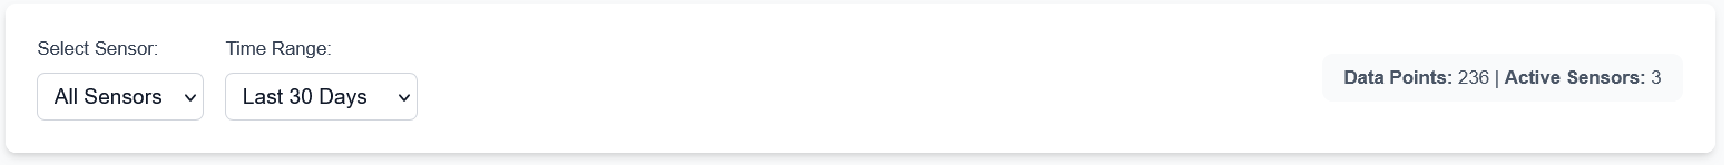
\includegraphics[width=\textwidth]{images/dashboard-control.png}
  % RENAME: image24.png → dashboard-control.png
\end{figure}

\begin{figure}[H]
  \caption{Visualisasi Data}
  \label{fig:lamp-chart}
  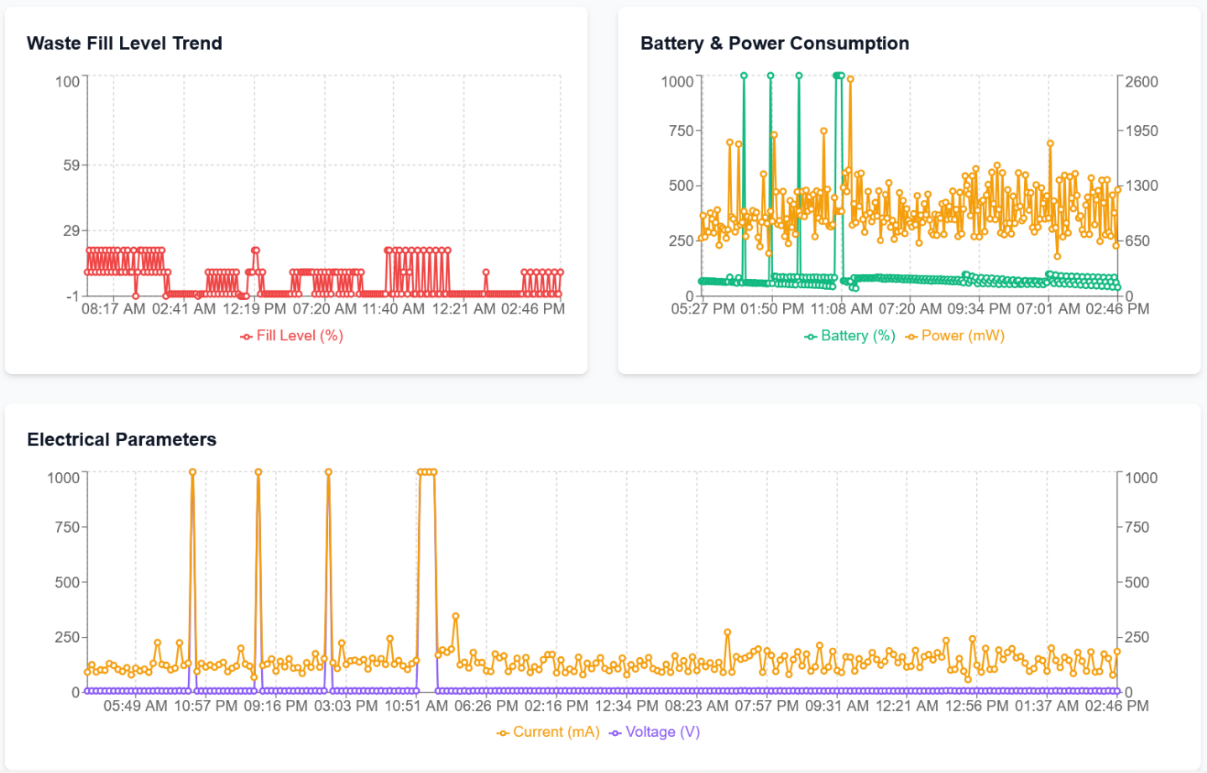
\includegraphics[width=\textwidth]{images/dashboard-chart.png}
  % RENAME: image25.png → dashboard-chart.png
\end{figure}

\begin{figure}[H]
  \caption{\textit{Recent Sensor Readings}}
  \label{fig:lamp-readings}
  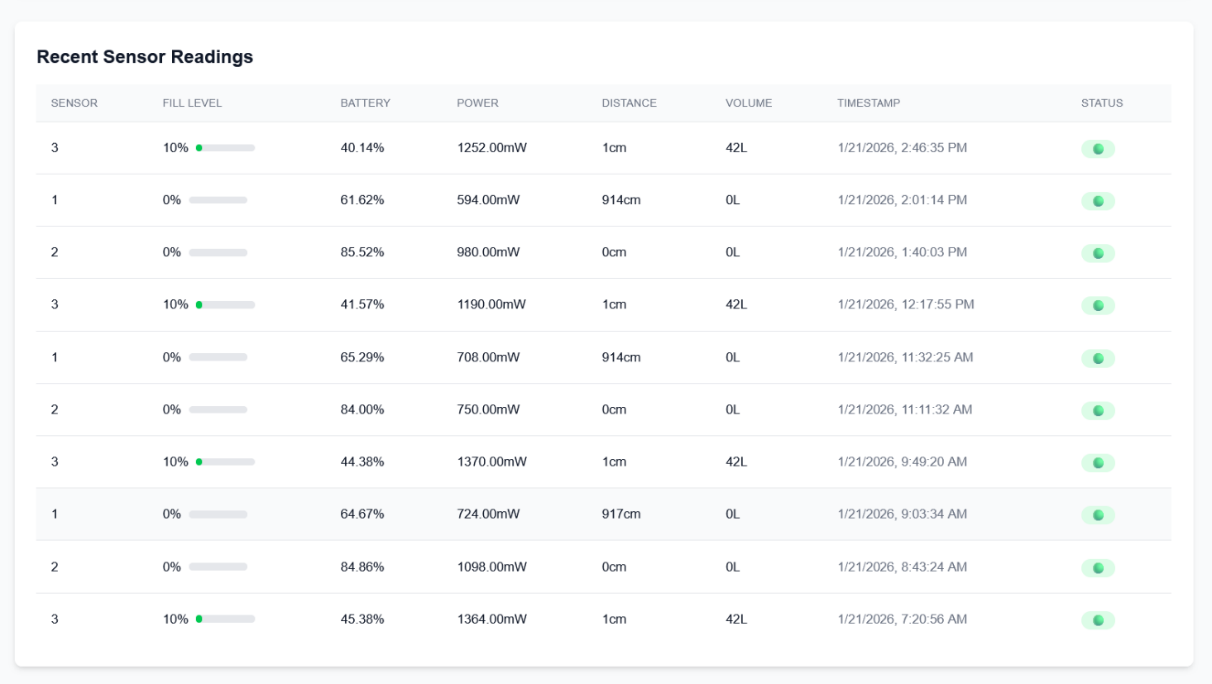
\includegraphics[width=\textwidth]{images/dashboard-readings.png}
  % RENAME: image26.png → dashboard-readings.png
\end{figure}

\begin{figure}[H]
  \caption{\textit{System Analytics}}
  \label{fig:lamp-analytics}
  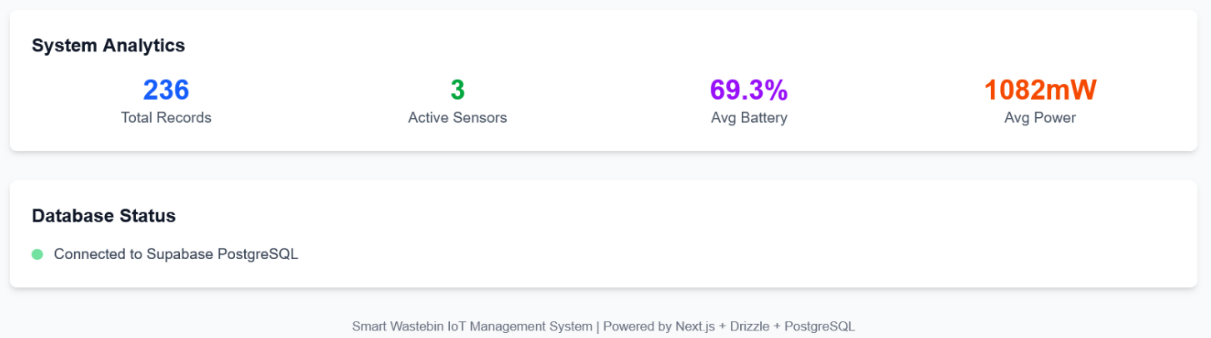
\includegraphics[width=\textwidth]{images/dashboard-analytics.png}
  % RENAME: image27.png → dashboard-analytics.png
\end{figure}
\chapter{BUKTI KESALAHAN PEMILAHAN SAMPAH OLEH PENGGUNA}
\label{chap:lampiran-c}

Lampiran ini mendokumentasikan bukti visual kesalahan pemilahan sampah yang ditemukan selama periode observasi lapangan. Temuan ini menjadi dasar rekomendasi program sosialisasi pemilahan sampah pada Subbab \ref{sec:saran}.

\section*{C.1 Sampah Anorganik Dibuang ke Tempat Sampah Organik}

\begin{figure}[H]
  \label{fig:lamp-c1a}
  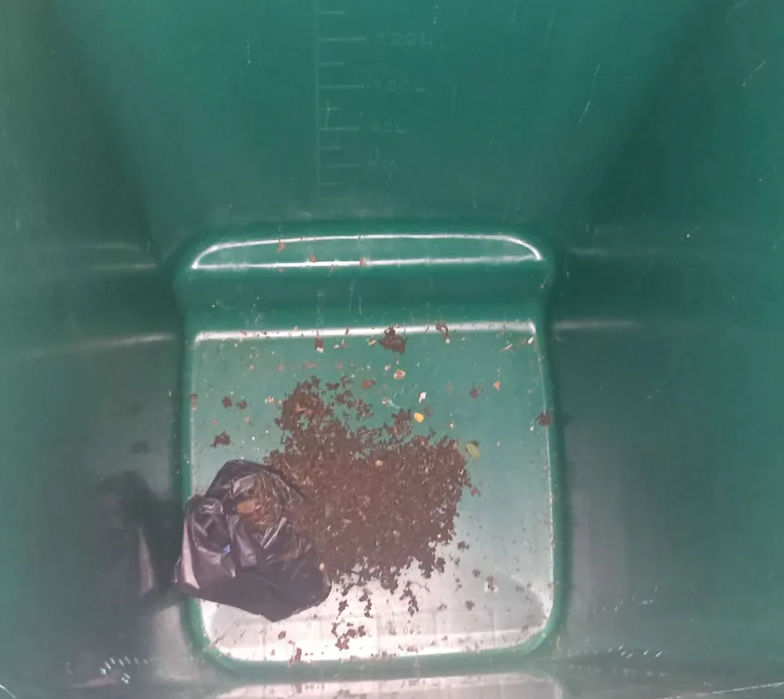
\includegraphics[width=0.75\textwidth]{images/salah-anorganik-ke-organik-1.png}
  \caption{Bukti 1: Sampah anorganik pada tempat sampah organik}
  % RENAME: image28.png → salah-anorganik-ke-organik-1.png
\end{figure}

\begin{figure}[H]
  \label{fig:lamp-c1b}
  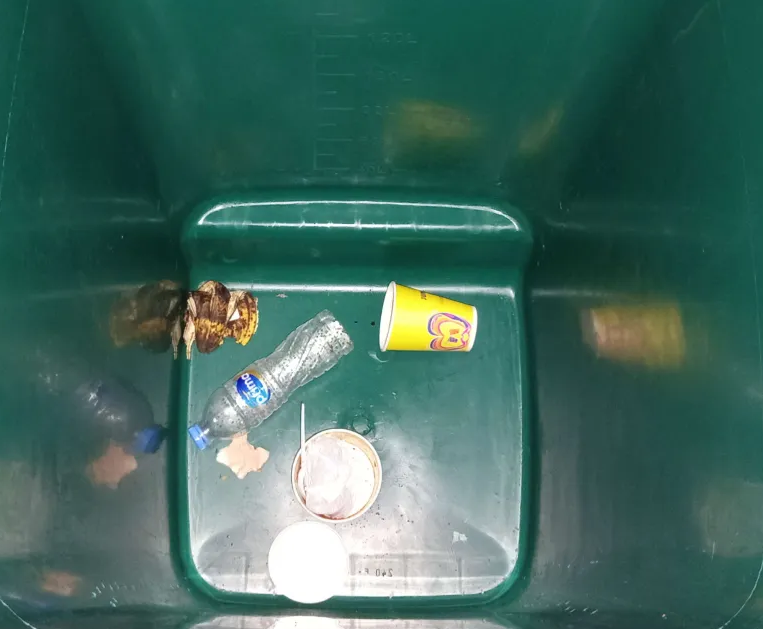
\includegraphics[width=0.75\textwidth]{images/salah-anorganik-ke-organik-2.png}
  \caption{Bukti 2: Sampah anorganik pada tempat sampah organik}
  % RENAME: image29.png → salah-anorganik-ke-organik-2.png
\end{figure}

\section*{C.2 Sampah Residu Dibuang ke Tempat Sampah Anorganik}

\begin{figure}[H]
  \label{fig:lamp-c2}
  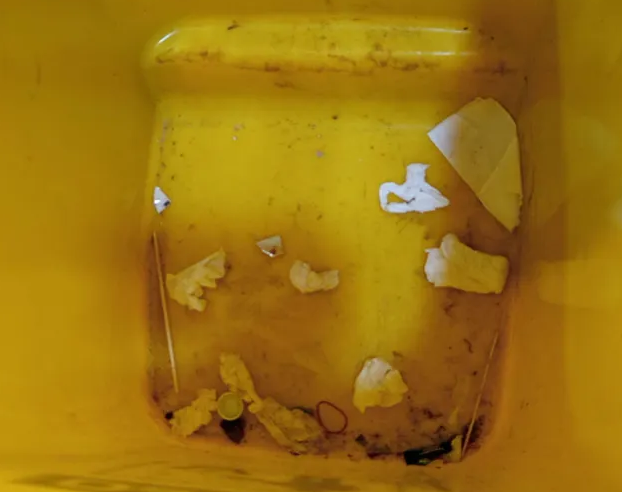
\includegraphics[width=0.65\textwidth]{images/salah-residu-ke-anorganik.png}
  \caption{Bukti: Sampah residu pada tempat sampah anorganik}
  % RENAME: image30.png → salah-residu-ke-anorganik.png
\end{figure}

\section*{C.3 Sampah Organik Dibuang ke Tempat Sampah Residu}

\begin{figure}[H]
  \label{fig:lamp-c3}
  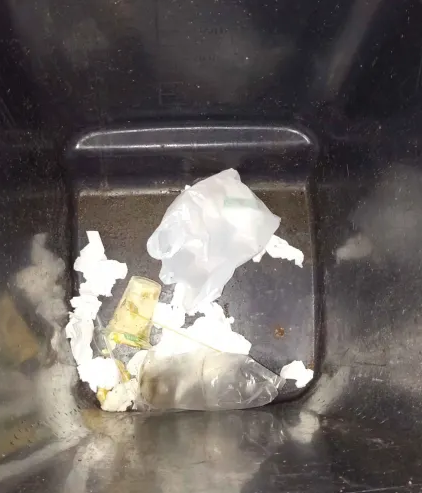
\includegraphics[width=0.75\textwidth]{images/salah-organik-ke-residu.png}
  \caption{Bukti: Sampah organik pada tempat sampah residu}
  % RENAME: image31.png → salah-organik-ke-residu.png
\end{figure}
\chapter{PEMASANGAN TEMPAT SAMPAH}
\label{chap:lampiran-d}

Lampiran ini mendokumentasikan proses pemasangan perangkat \textit{Smart Waste Bin} di lokasi pengujian pada Lantai 4 Gedung Labtek VIII ITB.

\section*{D.1 Pemasangan Roda Tempat Sampah}

\begin{figure}[H]
  \label{fig:lamp-d1}
  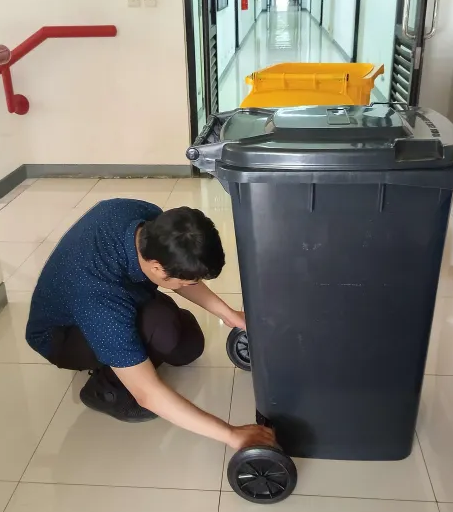
\includegraphics[width=0.75\textwidth]{images/pasang-roda.png}
  \caption{Pemasangan roda pada tempat sampah}
  % RENAME: image32.png → pasang-roda.png
\end{figure}

\section*{D.2 Pemasangan Baterai Perangkat IoT}

\begin{figure}[H]
  \label{fig:lamp-d2}
  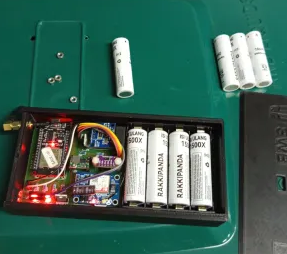
\includegraphics[width=0.65\textwidth]{images/pasang-baterai.png}
  \caption{Pemasangan baterai pada perangkat IoT}
  % RENAME: image33.png → pasang-baterai.png
\end{figure}

\section*{D.3 Pemasangan Perangkat IoT pada Tempat Sampah}

\begin{figure}[H]
  \label{fig:lamp-d3a}
  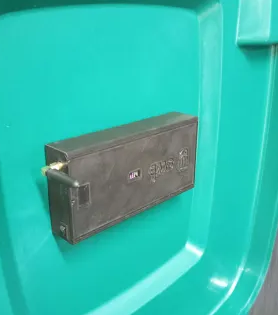
\includegraphics[width=0.65\textwidth]{images/pasang-iot-1.png}
  \caption{Pemasangan perangkat IoT pada tempat sampah (tampak depan)}
  % RENAME: image34.png → pasang-iot-1.png
\end{figure}

\begin{figure}[H]
  \label{fig:lamp-d3b}
  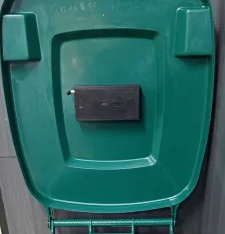
\includegraphics[width=0.65\textwidth]{images/pasang-iot-2.png}
  \caption{Pemasangan perangkat IoT pada tempat sampah (tampak samping)}
  % RENAME: image35.png → pasang-iot-2.png
\end{figure}

\section*{D.4 Pemasangan Label Tempat Sampah}

\begin{figure}[H]
  \label{fig:lamp-d4a}
  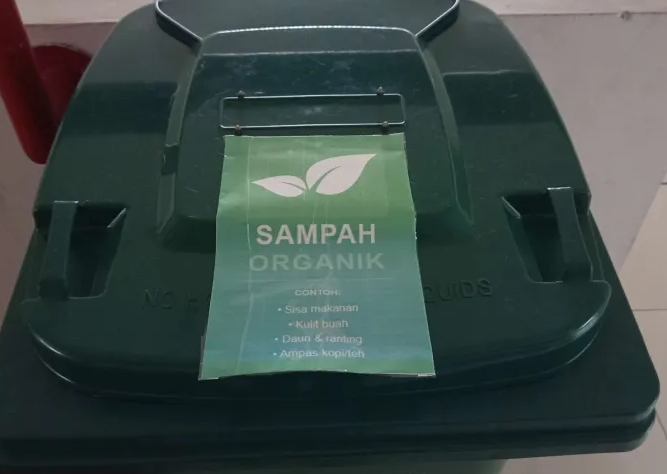
\includegraphics[width=0.75\textwidth]{images/pasang-label-1.png}
  \caption{Pemasangan label tempat sampah organik}
  % RENAME: image36.png → pasang-label-1.png
\end{figure}

\begin{figure}[H]
  \label{fig:lamp-d4b}
  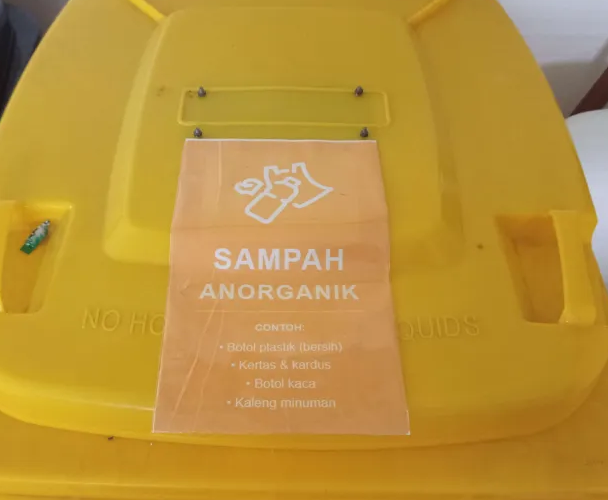
\includegraphics[width=0.75\textwidth]{images/pasang-label-2.png}
  \caption{Pemasangan label tempat sampah anorganik}
  % RENAME: image37.png → pasang-label-2.png
\end{figure}

\begin{figure}[H]
  \label{fig:lamp-d4c}
  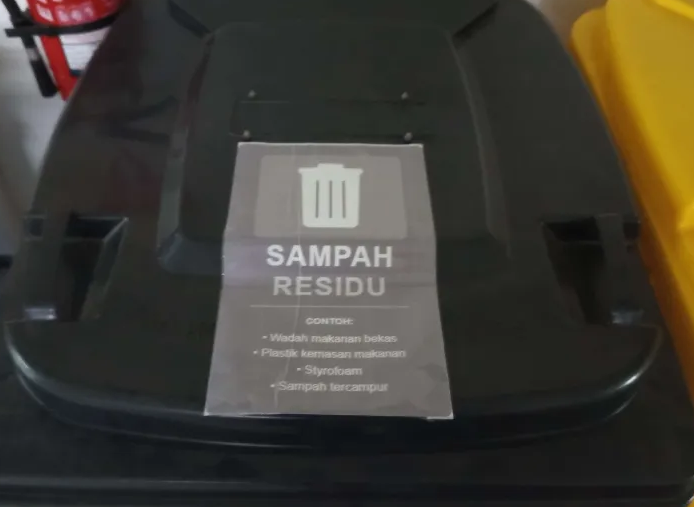
\includegraphics[width=0.75\textwidth]{images/pasang-label-3.png}
  \caption{Pemasangan label tempat sampah residu}
  % RENAME: image38.png → pasang-label-3.png
\end{figure}
\chapter{PERHITUNGAN AHP}
\label{chap:lampiran-e}

\section*{E.1 Normalisasi Matriks Perbandingan Kriteria}

\begin{table}[H]
  \caption{Normalisasi Matriks Perbandingan Kriteria}
  \label{tab:norm-kriteria}
  \centering
  \begin{tabular}{| l | c | c | c | c | c |}
    \hline
    & \textbf{C-1} & \textbf{C-2} & \textbf{C-3} & \textbf{C-4} & \textbf{Bobot ($w_i$)} \\
    \hline
    C-1 & 0,2703 & 0,2530 & 0,3158 & 0,3125 & 0,2879 \\
    \hline
    C-2 & 0,5405 & 0,5060 & 0,4737 & 0,4375 & 0,4894 \\
    \hline
    C-3 & 0,1351 & 0,1687 & 0,1579 & 0,1875 & 0,1623 \\
    \hline
    C-4 & 0,0541 & 0,0723 & 0,0526 & 0,0625 & 0,0604 \\
    \hline
    \textbf{Jumlah} & 1,0000 & 1,0000 & 1,0000 & 1,0000 & 1,0000 \\
    \hline
  \end{tabular}
\end{table}

\section*{E.2 Uji Konsistensi Matriks Kriteria}

Uji konsistensi dilakukan dengan menghitung \textit{Consistency Ratio} (CR). Langkah: (1) hitung vektor tertimbang $A \times w$, (2) hitung $\lambda$ per baris $= (A \times w)/w$, (3) $\lambda_{max}$ = rata-rata $\lambda$, (4) $CI = (\lambda_{max} - n)/(n-1)$, (5) $CR = CI/RI$.

\begin{table}[H]
  \caption{Uji Konsistensi Matriks Kriteria}
  \label{tab:uji-konsistensi-kriteria}
  \centering
  \begin{tabular}{| l | c | c | c |}
    \hline
    \textbf{Kriteria} & \textbf{Bobot ($w_i$)} & \textbf{$(A \times w)_i$} & \textbf{$\lambda_i = (A \times w)_i / w_i$} \\
    \hline
    C-1 & 0,2879 & 1,1591 & 4,0260 \\
    \hline
    C-2 & 0,4894 & 1,9747 & 4,0346 \\
    \hline
    C-3 & 0,1623 & 0,6505 & 4,0080 \\
    \hline
    C-4 & 0,0604 & 0,2420 & 4,0082 \\
    \hline
  \end{tabular}
\end{table}

Dengan $n = 4$ dan $RI = 0{,}90$:

\begin{align*}
  \lambda_{max} &= 4{,}019 \\
  CI &= \frac{\lambda_{max} - n}{n - 1} = \frac{4{,}0192 - 4}{4 - 1} = 0{,}0064 \\
  CR &= \frac{CI}{RI} = \frac{0{,}0064}{0{,}90} = 0{,}71\% < 10\% \quad \checkmark
\end{align*}

\section*{E.3 Matriks Perbandingan Alternatif per Kriteria}

\subsection*{E.3.1 C-1 (Kelayakan Teknis)}

\begin{table}[H]
  \caption{Matriks Berpasangan Alternatif --- C-1 (Kelayakan Teknis)}
  \label{tab:matriks-c1}
  \centering
  \begin{tabular}{| l | c | c | c | c |}
    \hline
    & \textbf{Alt-1} & \textbf{Alt-2} & \textbf{Alt-3} & \textbf{Bobot lokal ($w_i$)} \\
    \hline
    Alt-1 & 1     & 2   & 3 & 0,539 \\
    \hline
    Alt-2 & 1/2   & 1   & 2 & 0,297 \\
    \hline
    Alt-3 & 1/3   & 1/2 & 1 & 0,164 \\
    \hline
    \textbf{Jumlah kolom} & 1,833 & 3,500 & 6,000 & 1,000 \\
    \hline
  \end{tabular}
\end{table}

\begin{table}[H]
  \caption{Normalisasi dan Uji Konsistensi --- C-1 (Kelayakan Teknis)}
  \label{tab:norm-c1}
  \centering
  \begin{tabular}{| l | c | c | c | c | c |}
    \hline
    & \textbf{Alt-1} & \textbf{Alt-2} & \textbf{Alt-3} & \textbf{Bobot ($w_i$)} & \textbf{$\lambda_i$} \\
    \hline
    Alt-1 & 0,5455 & 0,5714 & 0,5000 & 0,5390 & 3,0147 \\
    \hline
    Alt-2 & 0,2727 & 0,2857 & 0,3333 & 0,2973 & 3,0085 \\
    \hline
    Alt-3 & 0,1818 & 0,1429 & 0,1667 & 0,1638 & 3,0044 \\
    \hline
  \end{tabular}
\end{table}

$\lambda_{max} = 3{,}0092$, $CI = 0{,}0046$, $RI = 0{,}58$, $CR = 0{,}79\% < 10\%$ $\checkmark$

\subsection*{E.3.2 C-2 (Kesesuaian Tujuan)}

\begin{table}[H]
  \caption{Matriks Berpasangan Alternatif --- C-2 (Kesesuaian Tujuan)}
  \label{tab:matriks-c2}
  \centering
  \begin{tabular}{| l | c | c | c | c |}
    \hline
    & \textbf{Alt-1} & \textbf{Alt-2} & \textbf{Alt-3} & \textbf{Bobot lokal ($w_i$)} \\
    \hline
    Alt-1 & 1 & 1/5 & 1/3 & 0,110 \\
    \hline
    Alt-2 & 5 & 1   & 2   & 0,581 \\
    \hline
    Alt-3 & 3 & 1/2 & 1   & 0,309 \\
    \hline
    \textbf{Jumlah kolom} & 9,000 & 1,700 & 3,333 & 1,000 \\
    \hline
  \end{tabular}
\end{table}

\begin{table}[H]
  \caption{Normalisasi dan Uji Konsistensi --- C-2 (Kesesuaian Tujuan)}
  \label{tab:norm-c2}
  \centering
  \begin{tabular}{| l | c | c | c | c | c |}
    \hline
    & \textbf{Alt-1} & \textbf{Alt-2} & \textbf{Alt-3} & \textbf{Bobot ($w_i$)} & \textbf{$\lambda_i$} \\
    \hline
    Alt-1 & 0,1111 & 0,1176 & 0,1000 & 0,1096 & 3,0012 \\
    \hline
    Alt-2 & 0,5556 & 0,5882 & 0,6000 & 0,5813 & 3,0064 \\
    \hline
    Alt-3 & 0,3333 & 0,2941 & 0,3000 & 0,3092 & 3,0035 \\
    \hline
  \end{tabular}
\end{table}

$\lambda_{max} = 3{,}0037$, $CI = 0{,}0018$, $RI = 0{,}58$, $CR = 0{,}32\% < 10\%$ $\checkmark$

\subsection*{E.3.3 C-3 (Waktu Pengembangan)}

\begin{table}[H]
  \caption{Matriks Berpasangan Alternatif --- C-3 (Waktu Pengembangan)}
  \label{tab:matriks-c3}
  \centering
  \begin{tabular}{| l | c | c | c | c |}
    \hline
    & \textbf{Alt-1} & \textbf{Alt-2} & \textbf{Alt-3} & \textbf{Bobot lokal ($w_i$)} \\
    \hline
    Alt-1 & 1   & 5 & 2   & 0,581 \\
    \hline
    Alt-2 & 1/5 & 1 & 1/3 & 0,110 \\
    \hline
    Alt-3 & 1/2 & 3 & 1   & 0,309 \\
    \hline
    \textbf{Jumlah kolom} & 1,700 & 9,000 & 3,333 & 1,000 \\
    \hline
  \end{tabular}
\end{table}

\begin{table}[H]
  \caption{Normalisasi dan Uji Konsistensi --- C-3 (Waktu Pengembangan)}
  \label{tab:norm-c3}
  \centering
  \begin{tabular}{| l | c | c | c | c | c |}
    \hline
    & \textbf{Alt-1} & \textbf{Alt-2} & \textbf{Alt-3} & \textbf{Bobot ($w_i$)} & \textbf{$\lambda_i$} \\
    \hline
    Alt-1 & 0,5882 & 0,5556 & 0,6000 & 0,5813 & 3,0064 \\
    \hline
    Alt-2 & 0,1176 & 0,1111 & 0,1000 & 0,1096 & 3,0012 \\
    \hline
    Alt-3 & 0,2941 & 0,3333 & 0,3000 & 0,3092 & 3,0035 \\
    \hline
  \end{tabular}
\end{table}

$\lambda_{max} = 3{,}0037$, $CI = 0{,}0018$, $RI = 0{,}58$, $CR = 0{,}32\% < 10\%$ $\checkmark$

\subsection*{E.3.4 C-4 (Biaya)}

\begin{table}[H]
  \caption{Matriks Berpasangan Alternatif --- C-4 (Biaya)}
  \label{tab:matriks-c4}
  \centering
  \begin{tabular}{| l | c | c | c | c |}
    \hline
    & \textbf{Alt-1} & \textbf{Alt-2} & \textbf{Alt-3} & \textbf{Bobot lokal ($w_i$)} \\
    \hline
    Alt-1 & 1 & 1   & 1/2 & 0,250 \\
    \hline
    Alt-2 & 1 & 1   & 1/2 & 0,250 \\
    \hline
    Alt-3 & 2 & 2   & 1   & 0,500 \\
    \hline
    \textbf{Jumlah kolom} & 4,000 & 4,000 & 2,000 & 1,000 \\
    \hline
  \end{tabular}
\end{table}

\begin{table}[H]
  \caption{Normalisasi dan Uji Konsistensi --- C-4 (Biaya)}
  \label{tab:norm-c4}
  \centering
  \begin{tabular}{| l | c | c | c | c | c |}
    \hline
    & \textbf{Alt-1} & \textbf{Alt-2} & \textbf{Alt-3} & \textbf{Bobot ($w_i$)} & \textbf{$\lambda_i$} \\
    \hline
    Alt-1 & 0,2500 & 0,2500 & 0,2500 & 0,2500 & 3,0000 \\
    \hline
    Alt-2 & 0,2500 & 0,2500 & 0,2500 & 0,2500 & 3,0000 \\
    \hline
    Alt-3 & 0,5000 & 0,5000 & 0,5000 & 0,5000 & 3,0000 \\
    \hline
  \end{tabular}
\end{table}

$\lambda_{max} = 3{,}0000$, $CI = 0{,}0000$, $RI = 0{,}58$, $CR = 0{,}00\% < 10\%$ $\checkmark$

\section*{E.4 Rincian Perhitungan Skor Global}

Skor global dihitung dengan rumus: $S(\text{Alt}_i) = \sum_j w_j \times w_{ij}$, di mana $w_j$ adalah bobot kriteria ke-$j$ dan $w_{ij}$ adalah bobot lokal alternatif $i$ pada kriteria $j$.

\begin{table}[H]
  \caption{Rincian Perhitungan Skor Global}
  \label{tab:skor-global-detail}
  \begin{tabularx}{\textwidth}{| l | X | X | X | X | c |}
    \hline
    \textbf{Alt} & \textbf{C-1 ($w$=0,288)} & \textbf{C-2 ($w$=0,489)} & \textbf{C-3 ($w$=0,162)} & \textbf{C-4 ($w$=0,060)} & \textbf{Skor Global} \\
    \hline
    Alt-1 & $0{,}539 \times 0{,}288 = 0{,}1552$ & $0{,}110 \times 0{,}489 = 0{,}0536$ & $0{,}581 \times 0{,}162 = 0{,}0943$ & $0{,}250 \times 0{,}060 = 0{,}0151$ & 0,318 (31,8\%) \\
    \hline
    Alt-2 & $0{,}297 \times 0{,}288 = 0{,}0856$ & $0{,}581 \times 0{,}489 = 0{,}2845$ & $0{,}110 \times 0{,}162 = 0{,}0178$ & $0{,}250 \times 0{,}060 = 0{,}0151$ & \textbf{0,403 (40,3\%)} \\
    \hline
    Alt-3 & $0{,}164 \times 0{,}288 = 0{,}0472$ & $0{,}309 \times 0{,}489 = 0{,}1513$ & $0{,}309 \times 0{,}162 = 0{,}0502$ & $0{,}500 \times 0{,}060 = 0{,}0302$ & 0,279 (27,9\%) \\
    \hline
  \end{tabularx}
\end{table}

\textbf{Alternatif 2} (SWB + \textit{Backend Custom} + \textit{Dashboard}) terpilih sebagai solusi terbaik dengan skor global tertinggi 0,403 (40,3\%).
\end{appendices}

\backmatter
\end{document}